\documentclass[12pt]{article}
\usepackage[a4paper, left=3cm, right=3cm, top=3cm, bottom=3cm]{geometry}
\usepackage[onehalfspacing]{setspace}
\usepackage{microtype}
\usepackage[T1]{fontenc}
\usepackage[utf8]{inputenc}
\usepackage[english, ngerman]{babel}
\usepackage{parskip} 
\usepackage{abstract}
\usepackage{float}
\usepackage{amsmath}
\usepackage{amstext}
\usepackage{varioref}
\usepackage[unicode=true,pdfusetitle,
 bookmarks=true,bookmarksnumbered=false,bookmarksopen=false, breaklinks=false,pdfborder={0 0 0},backref=false,colorlinks=false] {hyperref}
\hypersetup{
    colorlinks=true,
    linkcolor=blue,
    urlcolor=blue,
    citecolor=blue,
}
\usepackage{graphicx}
\usepackage{setspace}
\usepackage{lipsum}
\usepackage{cleveref}
\usepackage{icomma}
\usepackage{tabu,booktabs}
\usepackage{tcolorbox}
\usepackage{csquotes}
\usepackage{enumitem}
\usepackage{xspace}

\usepackage{tabularx}
\usepackage{pdflscape}
\usepackage{rotating}
\usepackage{booktabs}
\usepackage{array}
\newcolumntype{P}[1]{>{\centering\arraybackslash}p{#1}}
\renewcommand{\arraystretch}{1.1}
\usepackage{listings}
\usepackage{acronym}
\usepackage{minted}
\usepackage{longtable}
\usepackage{amssymb}
\usepackage{arabtex}
\usepackage{enumitem}
\setlist[itemize]{topsep=-0.2cm}
\usepackage[format=plain,
            font={it, small}]{caption}
\captionsetup{justification=raggedright,singlelinecheck=false}
\usepackage{threeparttable}
\usepackage{lastpage}
\usepackage{fancyhdr}
\pagestyle{fancy}
\fancyhead[R]{\nouppercase{\leftmark}}
\fancyhead[L]{}
\renewcommand{\headruleskip}{3pt}
\usepackage{afterpage}
\usepackage{tablefootnote}
\usepackage[hang,flushmargin]{footmisc}
%\usepackage{showframe}
% % % % % % % % % % % % % % % % % % % % %
%Schriften - nur eine auskommentieren
	%Latin Modern - Standard
\usepackage{lmodern}
	%Times Roman für strenge Dozenten
		%\usepackage{times}
	%Garamond - sieht toll aus, aber eher exotisch
		%\usepackage[cmintegrals,cmbraces]{newtxmath}\usepackage{ebgaramond-maths} %\usepackage{helvet}

%Hurenkinder, Schusterjungen
\widowpenalties=3 10000 10000 150

\newcommand*\MeasuredFigureLabel[1]{
    \addtocounter{figure}{-1}
    \phantomcaption
    \label{#1}
}

% % % % % % % % % % % % % % % % % % % % %
%LITERATUR
%Fußnote _ODER_ Amerikanisch auskommentieren

	%Amerikanische In-Text-Zitierweise
\usepackage[english]{babel}
\usepackage{csquotes}% Recommended
\usepackage[style=authoryear-ibid,backend=biber]{biblatex}


	%Deutsches Fußnotensystem
		%\usepackage[backend=biber,style=authortitle-dw,firstfull,maxcitenames=1]{biblatex}\DeclareFieldFormat{title}{\mkbibemph{#1}}\DeclareFieldFormat{citetitle}{\mkbibemph{#1}}\renewcommand{\cite}{\footcite}

%Ressource
\bibliography{bibtex.bib}
% for et. al. in italic
\usepackage{xpatch}
\xpatchbibmacro{name:andothers}{%
  \bibstring{andothers}%
}{%
  \bibstring[\emph]{andothers}%
}{}{}
% For using '&' insead of 'und' when \cite is used -> for text use \textcite
\DeclareDelimFormat[bib,cite]{finalnamedelim}{%
  \ifnumgreater{\value{liststop}}{2}{\finalandcomma}{}%
  \addspace\&\space}

% % % % % % % % % % % % % % % % % % % % %
\makeatletter


\begin{document}

%%Hier alle Daten einfügen
\newcommand{\autornameeins}{Marwin Ahnfeldt, B.Sc. ($819026$)}
\newcommand{\autornamezwei}{Tomas Kostadinov, B.Sc. ($820862$)}
\newcommand{\autornamedrei}{Laurenz Gilbert ($808291$)}
\newcommand{\autornamevier}{Jan-Hendrik Höltkemeier ($815258$)}
\newcommand{\autornamefuenf}{Victoria Schock ($797109$)}
\newcommand{\autornamesechs}{Fahian Arshad Bhuiyan ($806839$)}
\newcommand{\autornamesieben}{Eik Saathoff ($809906$)}
\newcommand{\fak}{Wirtschafts- und Sozialwissenschaftliche Fakultät}
\newcommand{\lehrstuhl}{Wirtschaftsinformatik, insb. Prozesse und Systeme}
\newcommand{\lv}{Analyse von Geschäftsprozessen \& Konzeption von IT Systemen (A\&K)}
\newcommand{\zeitraum}{Sommersemester 2023}
\newcommand{\lp}{M.Sc. Marcel Panzer}
\newcommand{\arbtyp}{Schaffung eines hochimmersiven (Lern-)Szenarios für hybride Simulationsumgebungen}
\newcommand{\titel}{ALAARM!}

\title{\titel}
\author{\autornameeins \autornamezwei \autornamedrei}

\newcommand{\TBA}{\texttt{\color{red}Todo}}
\begin{titlepage}
\vspace*{4.5cm}
\centering

\includegraphics[width=2.5cm]{res/uni_potsdam_logo.pdf}
\vfill
\begin{tabu} to \textwidth {X[c]}
	\huge{\textbf{{\textsc{\titel}}}}\\\\
	\large{\textsc{\arbtyp}}\\
\end{tabu}
\\[1cm]
\centering{
\autornameeins\\
\autornamesechs\\
\autornamedrei\\
\autornamevier\\
\autornamezwei\\
\autornamesieben\\
\autornamefuenf\\
}
\vfill
\begin{table}[h]
    \small
    \begin{tabular}{ll}
        Fakultät: & \fak \\
        Lehrstuhl: & \lehrstuhl \\
        Lehrveranstaltung: & \lv \\
        Bearbeitungszeitraum: & \zeitraum \\
        Dozent: & \lp
    \end{tabular}
\end{table}

\end{titlepage}

\renewcommand{\thepage}{\Roman{page}}
\setcounter{page}{1}
{\small\tableofcontents}
\cleardoublepage


\pagebreak{}
\selectlanguage{english} 
\renewcommand{\listfigurename}{Abbildungsverzeichnis}
% Abbildungsverzeichnis
\cleardoublepage
\listoffigures
\newpage
\pagebreak{}
\begin{abstract}
Die vorliegende Dokumentation bietet einen Einblick in das Studienprojekt \textit{ALAARM-ZIP}, welches das Ziel verfolgt, ein immersives Alarmszenario für eine hybride Industrie 4.0-Simulationsumgebung zu konzipieren und zu realisieren. Neben der Darstellung von Lösungsansätzen wie Alarmplänen und Simulationsumgebungen in anderen Branchen und Themenbereichen wird die erstellte Simulationsumgebung sowie das entwickelte Simulationsszenario präsentiert. Mit Hilfe der geschaffenen Simulationsumgebung können Alarmszenarien im Kontext einer Industrie 4.0-Anlage simuliert werden. Diese Dokumentation bietet Anknüpfungspunkte für die technische Weiterentwicklung der Simulationsumgebung, insbesondere für die Entwicklung neuer Simulationsszenarien. Basierend auf den Ergebnissen können Forschungsvorhaben, die sich unter anderem mit der Untersuchung von Alarmszenarien und Notfällen in vernetzten Industrie 4.0-Anlagen und deren Auswirkungen auf die Umwelt beschäftigen, realisiert werden.    
\end{abstract}
\pagebreak


\renewcommand{\thepage}{\arabic{page}}
\setcounter{page}{1}
\fancyfoot[C]{Seite \thepage \hspace{1pt} von \pageref*{LastPage}}

\setcounter{page}{1}


\pagebreak

\selectlanguage{ngerman} 


\onehalfspacing

%\section{Einleitung}
% 1-2 Seiten
Die Industrie 4.0, auch bekannt als die vierte industrielle Revolution, hat eine neue Ära der Automatisierung und Vernetzung in der Fertigung eingeläutet. Mit dem Ziel, Effizienz, Flexibilität und Produktivität zu steigern, werden in der Industrie 4.0 vernetzte Systeme eingesetzt, die eine nahtlose Kommunikation und Koordination zwischen Maschinen, Anlagen und Menschen ermöglichen \autocite{reinheimer}.

Die hohe Komplexität dieser Systeme stellt Mitarbeiter, wie beispielsweise Anlagenbediener, vor neue Herausforderungen. Insbesondere Alarmszenarien sind im Kontext der Industrie 4.0 eine bedeutende Problematik. Durch die Vernetzung und Koordination zwischen den Maschinen(-gruppen) kann eine einzelne Störung rasch ganze Fertigungsprozesse beeinträchtigen und zu einer Kaskade von Unterbrechungen und Folgestörungen führen. Um Schäden zu vermeiden und Sicherheit zu gewährleisten, trägt das Bedienungspersonal die Verantwortung, schnell und angemessen zu reagieren und Entstörungsmaßnahmen zu treffen. Das Verhalten verantwortlicher Personen bei einem Störfall in Industrie 4.0 Produktionsumgebungen wurde im wissenschaftlichen Kontext bisher nur wenig untersucht.

Im Rahmen dieses Forschungsprojekts liegt der Fokus auf der Entwicklung von Alarmszenarien im Kontext der „Industrie 4.0“. Dafür wird eine Dokumentation eines Alarmszenarios in Form eines BPMN-Prozesses und Begleitdokumenten erstellt. Diese Dokumentation dient als Basis für die Entwicklung eines Minimum Viable Products (MVP). Der MVP wird in die Simulationsumgebung des Zentrums Industrie 4.0 am Lehrstuhl für Wirtschaftsinformatik, Prozesse und Systeme der Universität Potsdam integriert (nachfolgend \textit{Zentrum Industrie 4.0}). Das Alarmszenario simuliert dabei einen Störfall, den die Simulationsteilnehmer bewältigen müssen.

Ziel des Projekts ist es, die Immersion der Alarmszenarien durch den Einsatz spezifischer Komponenten zu intensivieren, um den Stresslevel der Teilnehmer zu erhöhen und ein realistisches Szenario zu bieten. Dies eröffnet Forschungsmöglichkeiten im Bereich der Mensch-Maschine-Interaktion im Industrie 4.0 Umfeld, wie z.B. die Bewertung von Reaktionsvermögen und Effektivität des individuellen Verhaltens der Teilnehmer in Gefahrensituationen. Zudem können die erstellten Alarmszenarien zur Entwicklung von Schulungsprogrammen und Übungen eingesetzt werden, um das Bewusstsein und die Fähigkeiten der Mitarbeiter im Umgang mit potenziellen Gefahren zu schärfen.

In den nachfolgenden Abschnitten werden die methodischen Ansätze, die Definition und Dokumentation des erstellten Alarmszenarios sowie die Einbindung des Szenarios in die Simulationsumgebung detailliert präsentiert. Abschließend werden die Implikationen dieser Forschung diskutiert.
\\

\label{section:name-}
 \clearpage
\section{Einleitung}
% 1-2 Seiten
Die Industrie 4.0, auch bekannt als die vierte industrielle Revolution, hat eine neue Ära der Automatisierung und Vernetzung in der Fertigung eingeläutet. Mit dem Ziel, Effizienz, Flexibilität und Produktivität zu steigern, werden in der Industrie 4.0 vernetzte Systeme eingesetzt, die eine nahtlose Kommunikation und Koordination zwischen Maschinen, Anlagen und Menschen ermöglichen \autocite{reinheimer}.

Die hohe Komplexität dieser Systeme stellt Mitarbeiter, wie beispielsweise Anlagenbediener, vor neue Herausforderungen. Insbesondere Alarmszenarien sind im Kontext der Industrie 4.0 eine bedeutende Problematik. Durch die Vernetzung und Koordination zwischen den Maschinen(-gruppen) kann eine einzelne Störung rasch ganze Fertigungsprozesse beeinträchtigen und zu einer Kaskade von Unterbrechungen und Folgestörungen führen. Um Schäden zu vermeiden und Sicherheit zu gewährleisten, trägt das Bedienungspersonal die Verantwortung, schnell und angemessen zu reagieren und Entstörungsmaßnahmen zu treffen. Das Verhalten verantwortlicher Personen bei einem Störfall in Industrie 4.0 Produktionsumgebungen wurde im wissenschaftlichen Kontext bisher nur wenig untersucht.

Im Rahmen dieses Forschungsprojekts liegt der Fokus auf der Entwicklung von Alarmszenarien im Kontext der „Industrie 4.0“. Dafür wird eine Dokumentation eines Alarmszenarios in Form eines BPMN-Prozesses und Begleitdokumenten erstellt. Diese Dokumentation dient als Basis für die Entwicklung eines Minimum Viable Products (MVP). Der MVP wird in die Simulationsumgebung des Zentrums Industrie 4.0 am Lehrstuhl für Wirtschaftsinformatik, Prozesse und Systeme der Universität Potsdam integriert (nachfolgend \textit{Zentrum Industrie 4.0}). Das Alarmszenario simuliert dabei einen Störfall, den die Simulationsteilnehmer bewältigen müssen.

Ziel des Projekts ist es, die Immersion der Alarmszenarien durch den Einsatz spezifischer Komponenten zu intensivieren, um den Stresslevel der Teilnehmer zu erhöhen und ein realistisches Szenario zu bieten. Dies eröffnet Forschungsmöglichkeiten im Bereich der Mensch-Maschine-Interaktion im Industrie 4.0 Umfeld, wie z.B. die Bewertung von Reaktionsvermögen und Effektivität des individuellen Verhaltens der Teilnehmer in Gefahrensituationen. Zudem können die erstellten Alarmszenarien zur Entwicklung von Schulungsprogrammen und Übungen eingesetzt werden, um das Bewusstsein und die Fähigkeiten der Mitarbeiter im Umgang mit potenziellen Gefahren zu schärfen.

In den nachfolgenden Abschnitten werden die methodischen Ansätze, die Definition und Dokumentation des erstellten Alarmszenarios sowie die Einbindung des Szenarios in die Simulationsumgebung detailliert präsentiert. Abschließend werden die Implikationen dieser Forschung diskutiert.
\\

\label{section:name-}
 \clearpage
\section{Recherche}

\subsection{Recherche nach kommerziellen Lösungen}
Im Bereich des Maschinenbaus sind vielerlei \textbf{kommerzielle Lösungen} von Alarmsystemen zu nennen. Die folgenden Produktangebote und -hersteller bieten durch zusätzliche Hardware eine Echtzeitüberwachung an:
\begin{description}
    \item [\textbf{HGP-Eberle:}] 
    Cloud Alarmierungssystem mit permanenter Überwachung durch eine an die Maschine angeschlossene Alarm-Box. Im Störungsfall wird zuständiges Personal sofort per App benachrichtigt. (\cite{HGP-Eberle})
   
   \item [\textbf{Ixon-Cloud:}] 
   Webbasiertes Alarmierungssystem alarmiert Empfänger überall auf der Welt. Maschinen werden dabei durch ein Edge-Gerät kontinuierlich vor Ort überwacht und es wird eine Datenanalyse durchgeführt. (\cite{Ixon-Cloud})
   
   \item [\textbf{Mobeye:}] 
   Durch ein Gerät wird die Stromversorgung der Maschine überwacht. Bei einer Störung wird eine Alarmbenachrichtigung per App oder durch andere mobile Kommunikationswege versendet. Bei Push-Nachrichten lässt sich zudem zwischen verschiedenen Benachrichtigungsabläufen wählen. (\cite{Mobeye})
   
   \item [\textbf{Totmannschalter:}] 
   Ein Gerät überwacht eine allein arbeitende Person. Die Person kann einen manuellen Alarm auslösen, um einen Notruf abzugeben. Stellt das Gerät fest, dass die Person nicht handlungsfähig ist, wird automatisch ein Notruf ausgelöst. Per GPS-Ortung wird die Person lokalisiert. (\cite{totmann})
\end{description}
 
\

Des Weiteren ist zwischen den folgenden kommerziellen Benachrichtigungssystemen zu unterscheiden:
\begin{description}
   \item [\textbf{Workerbase:}] Die Maschinenalarm-App zeigt Maschinenausfälle als Warnung auf persönlichen Geräten der Mitarbeiter an. Dabei existieren verschiedene Alarmierungs- und Benachrichtigungsfunktionen für unterschiedliche Störungs- und Notfallsituationen. Mit den im Workerbase-System gesammelten Daten können über die App weitere Datenanalysen durchgeführt werden. (\cite{Workerbase})
   
   \item [\textbf{safeREACH:}] Über eine App können in verschiedenen Notfallsituationen alle betroffenen Personen kontaktiert und mit Informationen versorgt werden. Das Auslösen eines Alarms erfolgt per Knopfdruck oder durch Einbindung von Drittsystemen automatisch. Nach der Alarmierung stehen zudem weitere Tools zur Verfügung, um die Situation mit den richtigen Maßnahmen zu bewältigen. Die Aktivitäten werden automatisch protokolliert. (\cite{safeREACH})
   
   \item [\textbf{Vedosign:}] Durch einen per Knopfdruck ausgelösten Alarm wird eine standortbezogene Textnachricht an diverse mobile Geräte versendet. Die zielgerichtete Nachricht erlaubt die Benachrichtigung des richtigen Mitarbeiters, um präziser auf Alarme zu reagieren. (\cite{vedosign})
   
   \item [\textbf{Everbridge:}] Die Software macht es möglich, in sehr kritischen Gefahrensituationen eine Massennachricht über mehr als 25 Kontaktwege zu versenden. (\cite{everbridge})

   \item [\textbf{Gisbo:}] Diese Alarmierungssoftware unterstützt das Krisenmanagement in Gefahrensituationen. Verschiedene Alarmtypen können ausgelöst und Informationen schnell kommuniziert werden. Die Meldungen können akustisch und optisch sein, und werden über vorhandene IT-Infrastrukturen weitergeleitet. (\cite{Gisbo})

   \item [\textbf{WEKA:}] Elektroakustische Notfallsysteme (nach DIN EN 50849) warnen in Notfallsituationen anwesende Personen und fordern zu Selbstrettung auf. Durch unterschiedliche Signaltöne, die durch bspw. Sirenen übertragen werden, können Prioritäten im Vorfeld festgelegt und gespeicherte Alarmtexte wiedergegeben werden. (\cite{WEKA})
   
   \item [\textbf{Videc:}] Über das System werden sofortige und gezielte Benachrichtigungen an beteiligte Empfänger per E-Mail, SMS, Sprachnachricht, Audio, Messenger oder Pager versendet. Die Software fügt sich dabei in die vorhandene IT-Architektur des Unternehmens ein. (\cite{VIDEC})

   \item[ISA Telematics:] Das Angebot des Anbieters für Personen-Notsignal-Anlagen und Alleinarbeiterschutz umfasst die Sicherheits-App iTProtection, über welche Notsignale ausgelöst und Personen geortet werden können, und  die Telematikplattform iTelematics HL, über die Alarmmeldungen verwaltet werden können. Der Anwender wird über die Plattform akustisch über eine Alarmmeldung informiert und kann nach Anerkennung der Meldung auf hinterlegte Alarmpläne oder die Person betreffende medizinische Informationen zurückgreifen. (\cite{ISA_Telematics})

\end{description} \ 

\newpage
\subsection{Recherche nach Übungsszenarien und Standardabläufen}

In verschiedenen Zusammenhängen wurden Richtlinien, Handbücher und Empfehlungen zum \textbf{Inhalt und der Durchführung von Sicherheitsübungen} festgehalten. \\
Grundsätzlich wird dabei zwischen zwei Arten von Übungen unterschieden:
\begin{itemize}
    \item \textbf{Simulations- oder Stabsrahmenübungen: } Üben von Führungsfunktionen und Aufgaben von Einsatzkräften in geschlossenen Räumen (->strategische Entscheidungen). Diese Übungen sind mit weniger Aufwand verbunden, dadurch aber realitätsferner.   
    \item \textbf{Vollübungen: }Reales Handeln der Übungsteilnehmer. Das gesamte Einsatzgeschehen wird innerhalb der Übung möglichst realitätsnah abgebildet.
\end{itemize}\ 


Der „Leitfaden für strategische Krisenmanagement-Übungen“ vom \textbf{Bundesamt für Bevölkerungsschutz und Katastrophenhilfe} (\cite{strat_KrisenMGMT}) soll der effektiven Vorbereitung auf eine Krisensituation dienen. Angewendet werden die Inhalte unter anderem bei der Länder- und Ressortübergreifende Krisenmanagementübung (LÜKEX), die in regelmäßigen Abständen in Deutschland durchgeführt wird. \\
Der Ablauf einer solchen strategischen Krisenübung lässt sich in vier Abschnitte unterteilen:

\begin{itemize}
    \item \underline{Übungsplanung:}
    Es erfolgt eine konzeptionelle Vorbereitung. Im Übungsrahmen, dem zentralen Dokument, wird das Thema, die Beteiligten, Ziele, Organisationseinheiten und Kosten der Übung festgelegt. Es wird ein grobes Übungsszenario entwickelt und die Grundzüge der Übungsauswertung werden gesetzt.  \
    
    \item \underline{Übungsvorbereitung:}
    Es erfolgt der Aufbau der Übungssteuerung, des Kommunikationsplans und es wird das Konzept des Übungsszenarios weiterentwickelt. Dabei wird ein Drehbuch entwickelt, welches den chronologischen Verlauf der Übung festhält. Die Kernelemente des Szenarios sind dabei der allgemeine Hintergrund, die fiktive Ausgangslage, die fiktive Lageentwicklung, und jegliche Annahmen und Besonderheiten. Des Weiteren wird ein Auswertungskonzept inkl. Auswertungsunterlagen entwickelt und die Inhalte der Vorbesprechung und Anweisungen für Teilnehmende bestimmt.\

    \item \underline{Übungsdurchführung:}
    Vor der Durchführung ist eine Abstimmung aller Maßnahmen essenziell, um Missverständnisse zu vermeiden. Es erfolgt anschließend eine Lageeinweisung aller Beteiligten in ihre Rollen und die Überprüfung der Technik. Im Anschluss kann die geplante Übung durchgeführt und dokumentiert werden. 
    Bei frei verlaufenden Übungen soll keine Korrektur der Entscheidungen erfolgen und die Übung soll auch bei abweichendem Verlauf nicht unterbrochen werden, solange die fiktive Lage und das Szenario beachtet werden.
\

    \item \underline{Übungsauswertung:}
    Nach dem Durchlauf der Übung werden Erfahrungsberichte, Dokumentation, Fragebögen und Berichte von Beobachtern in einem zentralen Workshop behandelt und ein Auswertungsbericht erstellt.\\    

\end{itemize} 


Der Behelf für das „Anlegen und Durchführen von Einsatzübungen“ des \textbf{Bundesamts für Bevölkerungsschutz der Schweizerischen Eidgenossenschaft} \autocite{Behelf_Einsatzübungen} ist eine Unterlage, die zur Ausbildung dient und neben der Anleitung auch Formulare und Textvorlagen zur Verfügung stellt. \\
Der erste Teil der Anleitung behandelt das Anlegen einer Übung. Es wird der Bedarf für eine Übung wird ermittelt und es werden Thema, Ziele, Gelände sowie Übungsobjekte der Übung bestimmt. Anschließend wird das Konzept erstellt. Das Konzept soll auf Ausführbarkeit überprüft, und je nach Bedarf nur als Konzept oder auch mit detaillierteren Unterlagen dokumentiert werden. \\
Der zweite Teil geht auf die Durchführung einer Übung ein. Die Übungsleitung wird mit klar zugewiesenen Aufgabenbereichen eingeteilt, wobei die Beteiligten die nötige Fachkompetenz aufweisen sollten. Kommunikationsmittel und genutzte Markierungen/Signaturen müssen festgelegt sein. Dem Durchführen einer Übung folgt eine Besprechung, die eine Bilanzierung, Erläuterung von Zusammenhängen, Bewertung und Würdigung der Arbeit, und darauffolgende künftige Lehren behandeln soll. Die durchgeführte Übung wird anschließend mit der AEK-Methode (Aussage-Erkenntnis-Konsequenz) ausgewertet. \ 


Das \textbf{Deutsche Rote Kreuz} bietet im Buch „Durchführung und Auswertung von MANV-Übungen“ \autocite{MANV-Übungen} eine Bandbreite an Konzepten und Umsetzungshilfen für Übungen in Bezug auf das Szenario des Massenanfalls von Verletzten (MANV).
Auch hier beginnt der Übungsablauf mit der Planung. Ziele, Schadenslage, Einsatzmittel und Verlauf, und das Budget werden festgelegt. \\
In der anschließenden Vorbereitung werden Beteiligte benannt und die Kommunikation abgestimmt. Da bei dieser Art von Übung eine hohe Zahl an „Mimen“ (Figuranten, die im Szenario verletzte Personen darstellen) nötig ist, erfolgt in diesem Schritt die Registrierung und Terminabklärung, sowie die Erstellung eines Zeitplans des Übungstages. \\

\ 

Im nächsten Schritt folgt die Durchführung der Übung. Es erfolgt eine Einweisung und Sicherheitsbelehrung für die Beteiligten. Empfohlen werden pro Übung zwei Übungsläufe. \\
Nach der Durchführung erfolgt erst eine direkte Nachbereitung, bestehend aus einer Selbsteinschätzung und einer Vorstellung der Bewertungsindikatoren und Übungsdaten. Zuletzt folgt die spätere Nachbereitung, bei der die Übungsdaten in einer Führungskräftenachbesprechung evaluiert werden, und anschließend ein Abschlussbericht an alle Beteiligten versendet wird. \\

Das Begleitheft zur Unterstützung der Unfallverhütung beim Übungs- und Schulungsdienst der \textbf{Arbeitsgemeinschaft der Feuerwehr-Unfallkassen} \autocite{Feuerweh-Unfallkasse} nennt ebenfalls einen empfohlenen Ablauf einer Einsatzübung, der sich im Allgemeinen mit den bereits aufgeführten Inhalten gleicht. \\
Es erfolgt eine Übungsvorbereitung mit Gefährdungsbeurteilung, technischer und organisatorischer Planung, und Vorbesprechung. Darauf folgt die Durchführung und anschließend wird eine Nachbereitung mit Nachbesprechung und Auswertung durchgeführt. \\ 
Zusätzlich sind Hinweise bez. der Übungsdurchführung genannt: \\
Der Übungsort soll auf Gefahrenquellen überprüft und ausreichend beleuchtet sein, die Ausrüstung soll vor Beginn überprüft werden, Übungsteilnehmer sollen nicht überlastet werden und auf besonders gefährliche Handlungen soll verzichtet werden. Der Übung soll dabei dieselbe Aufmerksamkeit wie einem realen Einsatz geschenkt werden. \\
\textbf{Häufige Fehler} treten bei Einsatzübungen oft durch mangelnde Vorbereitung, falsche Annahmen, fehlender Berücksichtigung von vorhandenem Fachwissen und Einbeziehung nicht relevanter Faktoren auf. Außerdem werden oft Aufgabenbereiche im Vorhinein zu detailliert erläutert und Darstellungen unzureichend bzw. nicht erkennbar einbezogen. \autocite{Feuerweh-Übungspräsentation}

\ 

Ein weiterer Anwendungsbereich, indem Sicherheitsübungen erfolgen, ist das \textbf{Fahrsicherheitstraining}. Zwar ist Ablauf und Inhalt abhängig vom Veranstalter und Fahrzeugtyp, zum Großteil bestehen solche Übungen aus einem Theorie-Teil, einem Praxis-Teil und einer Nachbesprechung. \autocite{DVR}

\newpage
\subsection{Recherche nach wissenschaftlichen Studien}

\textbf{Es existieren bisher einige Projekte}, die immersive Software für das Training bzw. die Vorbereitung auf kritische Situationen getestet haben. So existiert bereits eine Lehrsoftware für Grundschullehrer, die mittels virtueller Realität das richtige Verhalten in Brandsituationen schulen soll. Die Software beinhaltet verschiedene Lernmechanismen wie dynamische Geschichten, Realismus, Bewegungsfreiheit, Level- und Punktsysteme \autocite{DDE_of_VR}. Im Industriellen Kontext existieren bereits Alarm- Management-Systeme, die in VR-Anwendungen für die Fertigung integriert worden sind. Das System dient zur besseren Handhabung von Alarmen und soll somit die Sicherheit von Arbeitnehmern verbessern. Das System kann Alarme automatisch auslösen und zeigt Benutzern visuelle Warnungen an, wenn ein Alarm ausgelöst wird \autocite{Design_of_VR-training}.

\textbf{Aufbauend sind zudem wissenschaftliche Studien} zu VR/AR-Anwendungen vorhanden, die untersuchen, ob und inwieweit sich die Vorbereitung auf Notfälle, die Reaktion während eines Notfalls und die Erholung nach einem Notfall durch den Einsatz von VR und AR-Anwendungen verbessert \autocite{VRandAR}. Einige Produktionsmaschinen und Systeme sind soweit vernetzt, dass sie die Maschinendaten selbständig auswerten und in der Cloud als 3D-Modell visualisieren lassen können. Die Maschine gibt also selber Rückmeldungen über ihren Status und kann ggf. Abweichungen und Fehler selbständig melden \autocite{Mascienenausf_entdecken}.

Ein interessanter Ansatz ist jedoch die Gerätewartung und Diagnose mittels Augmented Reality zu verbessern. Durch die Nutzung des Systems konnten Studierende Datenanalysen und -erfassung für Wartungsanwendungen leichter ausführen. Das Verständnis der Studierenden in diesem Sachbereich wurde durch die Einbindung von AR positiv beeinflusst (\cite{Develop_and_Asses_AR}). Für das ALAARM Projekt sind jedoch \textbf{Echtzeit-Fehlerdiagnosetechnologien (RTFD) für industrielle Prozessüberwachung und Maschinenzustandsüberwachung} besonders interessant. Diese Technologien finden zunehmend Einsatz in der industriellen intelligenten Fertigung und sollten daher unbedingt genauer betrachtet werden. Das im Rahmen des Projekts entworfene System bezieht sich in einem ausgedehnten Maße auf die dort bereits implementierten und entwickelten Technologien.

\newpage




\newpage

%\subsection{Literaturverweise}
%[1] Mystakidis, S., Besharat, J., Papantzikos, G., Christopoulos, A., Stylios, C., Agorgianitis, S. and Tselentis, D. (2022). Design, Development, and Evaluation of a Virtual Reality Serious Game for School Fire Preparedness Training. Education Sciences, 12(4), p.281. doi:https://doi.org/10.3390/educsci12040281. \\

%[2] Matsas, E. and Vosniakos, G. (2015). Design of a virtual reality training system for human–robot collaboration in manufacturing tasks. [online] Available at: https://www.researchgate.net/publication/271837242_Design_of_a_virtual_reality_training_s ystem_for_human-robot_collaboration_in_manufacturing_tasks [Accessed 18 May 2023]. \\


%[3] Zhu, Y. and Li, N. (2021). Virtual and Augmented Reality Technologies for Emergency Management in the Built Environments: A State-of-the-Art Review. Journal of Safety Science and Resilience, Volume 2(March 2021). doi:https://doi.org/10.1016/j.jnlssr.2020.11.004. \\


%[4] Weidle, D. (2023). Maschinenausfälle entdecken bevor sie auftreten. Maschinenausfälle entdecken bevor sie auftreten, 26(5), pp.26–27. doi:https://doi.org/10.1002/citp.202300515. \\

%[5] Shyr, W.-J., Tsai, C.-J., Lin, C.-M. and Liau, H.-M. (2022). Development and Assessment of Augmented Reality Technology for Using in an Equipment Maintenance and Diagnostic System. Sustainability, 14(19), p.12154. doi:https://doi.org/10.3390/su141912154. \\


%[6] Yan, W., Wang, J., Lu, S., Zhou, M. and Peng, X. (2023). A Review of Real-Time Fault Diagnosis Methods for Industrial Smart Manufacturing. Processes, 11(2), pp.369–369. doi:https://doi.org/10.3390/pr11020369.
 \clearpage
\section{Beschreibungskarte}

\ 

\textbf{AGENDA}

\ 

\textbf{3.1 Einleitung und Szenario-Überblick} 
\begin{itemize}
\item
Präsentation des Szenarios und seiner Komponenten
\item
Erklärung des Ablaufs und der Eskalationsstufen
\end{itemize}

\

\textbf{3.2 Sicherheitsbriefing} 
\begin{itemize}
\item
Durchsicht der Gesundheits- und Sicherheitshinweise
\end{itemize}

\

\textbf{3.3 Bedienungsanleitung und Aktivierung der Eskalationsstufe}
\begin{itemize}
\item
Erläuterung der Bedienung der Maschine und des Tablets
\item
Aktivierung der Eskalationsstufe 
\end{itemize}

\

\textbf{3.4 Anzeige der Fehlermeldung und Lösungsansatz }
\begin{itemize}
\item
Erläuterung der Schritte zur Lösung der Fehlermeldungen
\end{itemize}

\

\textbf{3.5 Eskalationsstufe 1}
\begin{itemize}
\item
Durchgehen der Eskalationsstufe 1 und der damit verbundenen Entstörungsvorgang
\item 
Einschreiten der Zufallsvariable
\item
Diskussion über die möglichen Auswirkungen der Zufallsvariable auf den Ausgang des Szenarios
\end{itemize}

\

\textbf{3.6 Eskalationsstufe 2}
\begin{itemize}
\item
Durchgehen der Eskalationsstufe 2 und der damit verbundenen Entstörungsvorgang
\item
Einschreiten der Zufallsvariable
\item
Diskussion über die möglichen Auswirkungen der Zufallsvariable auf den Ausgang des Szenarios
\end{itemize}

 \

\textbf{3.7 Eskalationsstufe 3}
\begin{itemize}
\item
Durchgehen der Eskalationsstufe 2 und der damit verbundenen Entstörungsvorgang
\item
Einschreiten der Zufallsvariable
\item
Diskussion über die möglichen Auswirkungen der Zufallsvariable auf den Ausgang des Szenarios
\end{itemize}

\

\textbf{3.8 Voraussichtliche Zeitangaben des Szenarios zum Abschluss}
\begin{itemize}
\item
Messung der Durchlaufzeit bei optimalen Abläufen
\end{itemize}

\newpage

\textbf{3.1 Einleitung und Szenario-Überblick}

In diesem Szenario wird ein komplexes System aus verschiedenen Komponenten und Prozessen beschrieben, dass in einen Maschinen-Simulationsraum implementiert wird. Die Szenariokomponenten bestehen aus Teilnehmer, Tablet, Subwoofer/Lautsprecher, Wärmelampe/Licht und Vaporizer. Diese Komponenten sind in einer Umgebung platziert, in der es Anlagen zum Bedienen gibt, die alle durch ein Förderband miteinander verbunden sind. Das System ist so konzipiert, dass es drei Eskalationsstufen gibt, die nacheinander aktiviert werden können. Jede Eskalationsstufe beinhaltet einen Entstörungsvorgang, der vom Teilnehmer gelöst werden muss. Dabei werden verschiedene Szenariokomponenten aktiviert, um den Prozess zu unterstützen und zu simulieren. Teilnehmer des Szenarios, die bei einem Enstörungsvorgang versagen, werden automatisch zur nächsten Eskalationsstufe befördert, bis sie maximal die Eskalationsstufe 3 erreichen. Während eines Enstörungsvorgangs steht den Teilnehmern dabei nur ein Versuch zur Verfügung. Allerdings haben erfolgreiche Szenarioteilnehmer die Möglichkeit, nach Abschluss einer beliebigen Eskalationsstufe das gesamte Szenario vorzeitig zu beenden. Pro Durchgang führt nur ein Szenarioteilnehmer das Szenario durch. Es gibt einen Betreuer, der diese Vorgänge beobachtet und bei Notfällen einschreitet, jedoch ist er nicht für die gesamten Handlungen im Szenarioprozess eingeplant.

\

\underline{Einleitung zum Szenario:} \\
Der Teilnehmer aktiviert die Anlage mit einem Startknopf auf dem Tablet. (Zeit: ca. 1 Sekunde)
Es wird das Datenpaket für den Szenarioteilnehmer ausgelesen, woraufhin Anweisungen wie Gesundheitswarnungen oder weitere Verfahren angezeigt werden, die der Teilnehmer lesen soll: (Zeit: ca. 2 Minute)

\

\textbf{3.2 Sicherheitsbriefing}

\emph{Bitte nehmen Sie sich die Zeit, diese Anweisungen sorgfältig zu lesen und zu verstehen, bevor Sie mit dem Betrieb der Maschine fortfahren. Ihre Sicherheit hat oberste Priorität.}

\newpage

\emph{WICHTIG: GESUNDHEITSWARNUNG \\
Bitte stellen Sie sicher, dass Sie die geeignete Schutzkleidung tragen, bevor Sie mit dem Betrieb dieser Maschine beginnen. Dies beinhaltet Schutzhandschuhe, Schutzbrille und Atemschutzmaske. Bitte entnehmen Sie die Schutzkleidung, die rechts von Ihnen lieg. 
Es besteht die Möglichkeit, dass während des Szenarios Rauch oder andere intensiv riechende Substanzen verwendet werden.
Dieses Szenario beinhaltet flackernde Lichter, die bei einigen Personen mit Epilepsie zu Anfällen führen können. 
Bitte beachten Sie, dass Ihre Gesundheit und Sicherheit oberste Priorität haben. Falls Sie Bedenken haben oder gesundheitliche Einschränkungen haben, die sich auf Ihre Teilnahme an diesem Szenario auswirken könnten, empfehlen wir Ihnen, vorab Rücksprache mit einem Arzt zu halten, um sicherzustellen, dass Sie angemessen geschützt sind und das Szenario ohne Risiken für Ihre Gesundheit durchführen können.}

\

\textbf{3.3 Bedienungsanleitung und Aktivierung der Eskalationsstufe}
\

\emph{BEDIENUNGSANLEITUNG \\
1.	Überprüfen Sie, ob alle Sicherheitsvorkehrungen getroffen wurden und die Maschine bereit für den Betrieb ist. \\
2.	Drücken Sie den grünen Startknopf auf der rechten Seite des Bedienfelds, um den Maschinenprozess zu starten. \\
3.	Überwachen Sie den Prozess auf dem Bildschirm. Achten Sie auf alle Warnungen oder Fehlermeldungen, die angezeigt werden könnten. \\
4.	Im Falle einer Fehlermeldung, drücken Sie den roten Stopp-Knopf und befolgen Sie die Anweisungen auf dem Bildschirm. \\
5.	Wenn der Prozess abgeschlossen ist, drücken Sie den blauen Reset-Knopf, um die Maschine auf ihren Ausgangszustand zurückzusetzen.}

\

\textbf{\underline{Start:}}

\

\underline{Einleitung der Eskalationsstufe 1:}

Die Anlage fängt an zu laufen. (Zeit: ca. 8 Sekunden) 
Gleichzeitig werden in der ersten Stufe die Szenariokomponenten aktiviert, wie der Subwoofer/Lautsprecher, der einen langsamen pulsierenden Ton erzeugt, sowie die Wärmelampe/Licht (Andon-Signalleuchte), die an der jeweiligen Maschine aktiviert wird und kontinuierlich leuchtet. (Zeit: ca. 1 Sekunde)
Die Anlage ruckelt und stoppt ihren Arbeitsfluss. (Zeit: ca. 5 Sekunden)

\

\textbf{3.4 Anzeige der Fehlermeldung und Lösungsansatz}

Auf dem Tablet erscheint ein Fehlercode mit dazugehörigen Maschinen- und Fehlerdetails, die der Szenarioteilnehmer liest: (Zeit: ca. 40 Sekunden)

\

\emph{FEHLERCODE: E101\\
BETROFFENE MASCHINE: Maschine 3\\
FEHLERDETAILS: Überhitzung}

\

\emph{Die Sensoren in Maschine 3 haben eine übermäßige Wärmeentwicklung festgestellt, die über den sicheren Betriebsbereich hinausgeht. Dies kann zu Schäden an der Maschine und möglicherweise zu einem unsicheren Arbeitsumfeld führen.}

\emph{Stoppen Sie Maschine 3 sofort, um weitere Schäden zu vermeiden, und lösen Sie das Rätsel während des Entstörungsvorgangs!}

Hinlaufen zu dieser Maschine. (Zeit: ca. 15 Sekunden)

\

\textbf{3.5 Eskalationsstufe 1}

Auf dem Tablet erscheint ein QR-Code, der gescannt werden muss, um einen Entstörungsvorgang in 40 Sekunden bzw. das Problem zu lösen wie: (Zeit: ca. 45 Sekunden)

\emph{(!) Lösen Sie das folgende Rätsel, um den Fehler zu beheben!}

\

\underline{\emph{Nummernspiel}} \\
\emph{Auf dem Tablet wird eine Zahlenfolge angezeigt:} \\

\

\emph{(!) Lösen Sie das folgende Rätsel, um den Fehler zu beheben!} \\

\emph{Auf dem Tablet wird eine zufällige Zahlenfolge angezeigt:} \\
\emph{3, 5, 8, 10, 9, 2, 7, 4, 1, 6} \\

\
\emph{Ihre Aufgabe ist es, die Zahlen in aufsteigender Reihenfolge anzuklicken. Sie haben 10 Sekunden Zeit, um das Rätsel zu lösen.}

\

Es folgt eine Verzweigung, die eine Zufallsvariable beinhaltet:

{Nach erfolgreichem Abschluss des Entstörungsvorgangs wird auf dem Tablet eine Benachrichtigung angezeigt, die den Abschluss des Vorgangs bestätigt. Um die Wahrscheinlichkeit von 33\% zu simulieren, wird eine digitale Würfelfunktion verwendet, die die Zahlen 1, 2 und 3 generiert und damit drei mögliche Zustände repräsentiert. Nach dem Entstörungsvorgang wird die digitale Würfelfunktion ausgeführt. Wenn die gewürfelte Zahl eine 1 oder 2 ist (entspricht einer Wahrscheinlichkeit von 2/3), wird auf dem Tablet angezeigt, dass das Problem als gelöst erfasst wurde. Falls die gewürfelte Zahl eine 3 ist (entspricht einer Wahrscheinlichkeit von 1/3), wird auf dem Tablet angezeigt, dass das Problem nicht vollständig gelöst wurde. \\

\begin{itemize}
\item
Sollte der Entstörungsvorgang innerhalb der vorgegebenen Zeit nicht erfolgreich abgeschlossen werden oder eine falsche Eingabe getätigt werden, erfolgt der Übergang zur zweiten Eskalationsstufe automatisch. (Keine genaue Zeitangabe)
\item
Ist der Entstörungsvorgang erfolgreich gelöst, folgt die Zufallsvariable, dabei wird bei einer 1/3 Wahrscheinlichkeit das Problem als nicht gelöst erfasst. Dann erfolgt ebenfalls der Übergang zur zweiten Eskalationsstufe automatisch. (Keine genaue Zeitangabe)
\item
Wenn der Entstörungsvorgang erfolgreich gelöst ist, folgt die Zufallsvariable, bei der mit einer Wahrscheinlichkeit von 2/3 das Problem als gelöst erfasst wird. Wenn dieses Szenario eintrifft, werden alle Szenariokomponenten ausgeschaltet und das Szenario für den Teilnehmer ist erfolgreich beendet.  (Zeit: ca. 3 Sekunden)
\end{itemize}


\newpage 

\textbf{3.6 Eskalationsstufe 2}

Simultan werden die Szenariokompontenten Subwoofer/Lautprecher mit einem mittelschnell schlagenden Ton aktiviert. Der Vaporizer stößt derweil Brandgeruch aus. Die LED-Leuchte flackert bei der Maschine blau. Diese bleiben durchgehend in der zweiten Eskalationsstufe aktiv. (Zeit: ca. 5 Sekunde) \\
Der Szenarioteilnehmer soll sich selbstständig zur nächsten Maschine bewegen, was durch eine Andon-Signalleuchte an der Maschine signalisiert wird. (Zeit: ca. 15 Sekunden) \\
Erneut muss ein Entstörungsvorgang durchgeführt werden: (Zeit: ca. 40 Sekunden) 

\

\underline{\emph{Kalibrierung}} \\
\emph{(!) Lösen Sie das folgende Rätsel, um den Fehler zu beheben!}\\

Es gibt ein Problem mit der Kalibrierung der Maschine, was zu schwerwiegenden Fehlfunktionen führt. Es ist entscheidend, dass die Eingaben der Maschine korrekt kalibriert sind, um Fehlerquellen zu eliminieren. Um eine korrekte Kalibrierung zu gewährleisten, klicken Sie so schnell wie möglich auf den Bildschirm, sobald er grün wird. \\
          
Der Bildschirm startet im schwarzen Zustand. Wenn Sie länger als 0,6 Sekunden brauchen, um eines der beiden grünen Kacheln anzuklicken, kann die Maschine nicht kalibriert werden. Es sind 6 Kalibrierungseingaben erforderlich, um die Maschine erfolgreich zu kalibrieren.

$\Box\hspace{85pt}\\\Box$

\

Danach erfolgt eine weitere Verzweigung, bei der die Zufallsvariable aktiviert wird. \\

\

\textbf{3.7 Eskalationsstufe 3} \\

Gleichzeitig werden die Szenariokomponenten Subwoofer/Lautsprecher mit einem schnell schlagenden Ton, der Vaporizer mit einem intensiveren Geruch als zuvor und die Wärmelampe aktiviert. Die Andon-leuchte flackert rot. Diese bleiben durchgehend in der dritten Eskalationsstufe aktiv. (Zeit: ca. 5 Sekunde) \\
Der Szenarioteilnehmer soll zur nächsten Maschine, welches durch eine Andon-Signalleuchte signalisiert wird, hinbewegen. (Zeit: ca. 15 Sekunden) \\
Erneut muss ein Entstörungsvorgang durchgeführt werden: (Zeit: ca. 40 Sekunden) 

\

\underline{\emph{Algorithmus}} \\
\emph{Auf dem Tablet wird eine Zahlenfolge angezeigt:} \\

\

\emph{(!) Lösen Sie das folgende Rätsel, um den Fehler zu beheben!} \\

\
\emph{Der Algorithmus der Maschine scheint ein Problem zu haben. \\
Um die Maschine zu reparieren, müssen Sie die Zahlen 1 bis 10 in aufsteigender Reihenfolge anklicken.
Nach 5 und 10 Sekunden werden die Zahlen durcheinandergebracht. \\
Sobald Sie beginnen, haben Sie 15 Sekunden Zeit.}

\

\emph{Die Zahlen werden auf dem Bildschirm in einer zufälligen Reihenfolge verstreut angezeigt:} \\
\emph{3\hspace{15pt} 5\hspace{42pt} 8\hspace{58pt} 10\hspace{75pt} \\9\hspace{25pt} 2\hspace{37pt} 7\hspace{83pt} \\4\hspace{39pt} 1\hspace{66pt} 6\hspace{81pt}} \\

\
Danach erfolgt eine weitere Verzweigung, bei der die Zufallsvariable aktiviert wird.

\

\textbf{3.8 Voraussichtliche Zeitangaben des Szenarios}\\
Bitte beachten Sie, dass dies geschätzte Zeiten sind und je nach individueller Durchführung und Reaktionsgeschwindigkeit des Teilnehmers leicht variieren können. Diese Zeitangaben stehen daher unter Vorbehalt und dienen lediglich als grobe Orientierung. Es ist möglich, dass die tatsächliche Dauer für jeden Teilnehmer unterschiedlich ist.

\

\underline{Benötigte Zeit für Eskalationsstufe 1} \\
Lesen der Anweisungen: ca. 2 Minuten \\
Aktivierung der Anlage: ca. 8 Sekunden \\
Unterbrechung der Anlage ca. 5 Sekunden \\
Anzeige der Fehlermeldung: ca. 40 Sekunden \\
Hinlaufen zur Maschine: ca. 15 Sekunden \\
Entstörungsvorgang in der ersten Stufe: ca. 10 Sekunden \\
Einschreiten der Zufallsvariable: ca. 3 Sekunden \\
Geschätzte Gesamtzeit für den Abschluss der ersten Stufe: ca. 3 1/2 Minuten \\

\

\underline{Benötigte Zeit für Eskalationsstufe 2} \\
Zeit für die erste Stufe: ca. 3 1/2 Minuten \\
Hinlaufen zur Maschine: ca. 15 Sekunden \\
Entstörungsvorgang in der zweiten Stufe: ca. 40 Sekunden \\
Einschreiten der Zufallsvariable: ca. 3 Sekunden \\
Geschätzte Gesamtzeit für den Abschluss der ersten und der zweiten Stufe: ca. 4 1/2 Minuten \\

\

\underline{Benötigte Zeit für Eskalationsstufe 3 / Max. Zeit bei Erfolglosigkeit} \\
Zeit für die zweite Stufe: ca. 4 1/2 Minuten \\
Hinlaufen zur Maschine: ca. 15 Sekunden \\
Entstörungsvorgang in der dritten Stufe: ca. 15 Sekunden \\
Einschreiten der Zufallsvariable: ca. 3 Sekunden \\
Geschätzte Gesamtzeit für den Abschluss der ersten, zweiten und der dritten Stufe: ca. 5 Minuten \\




 \clearpage

%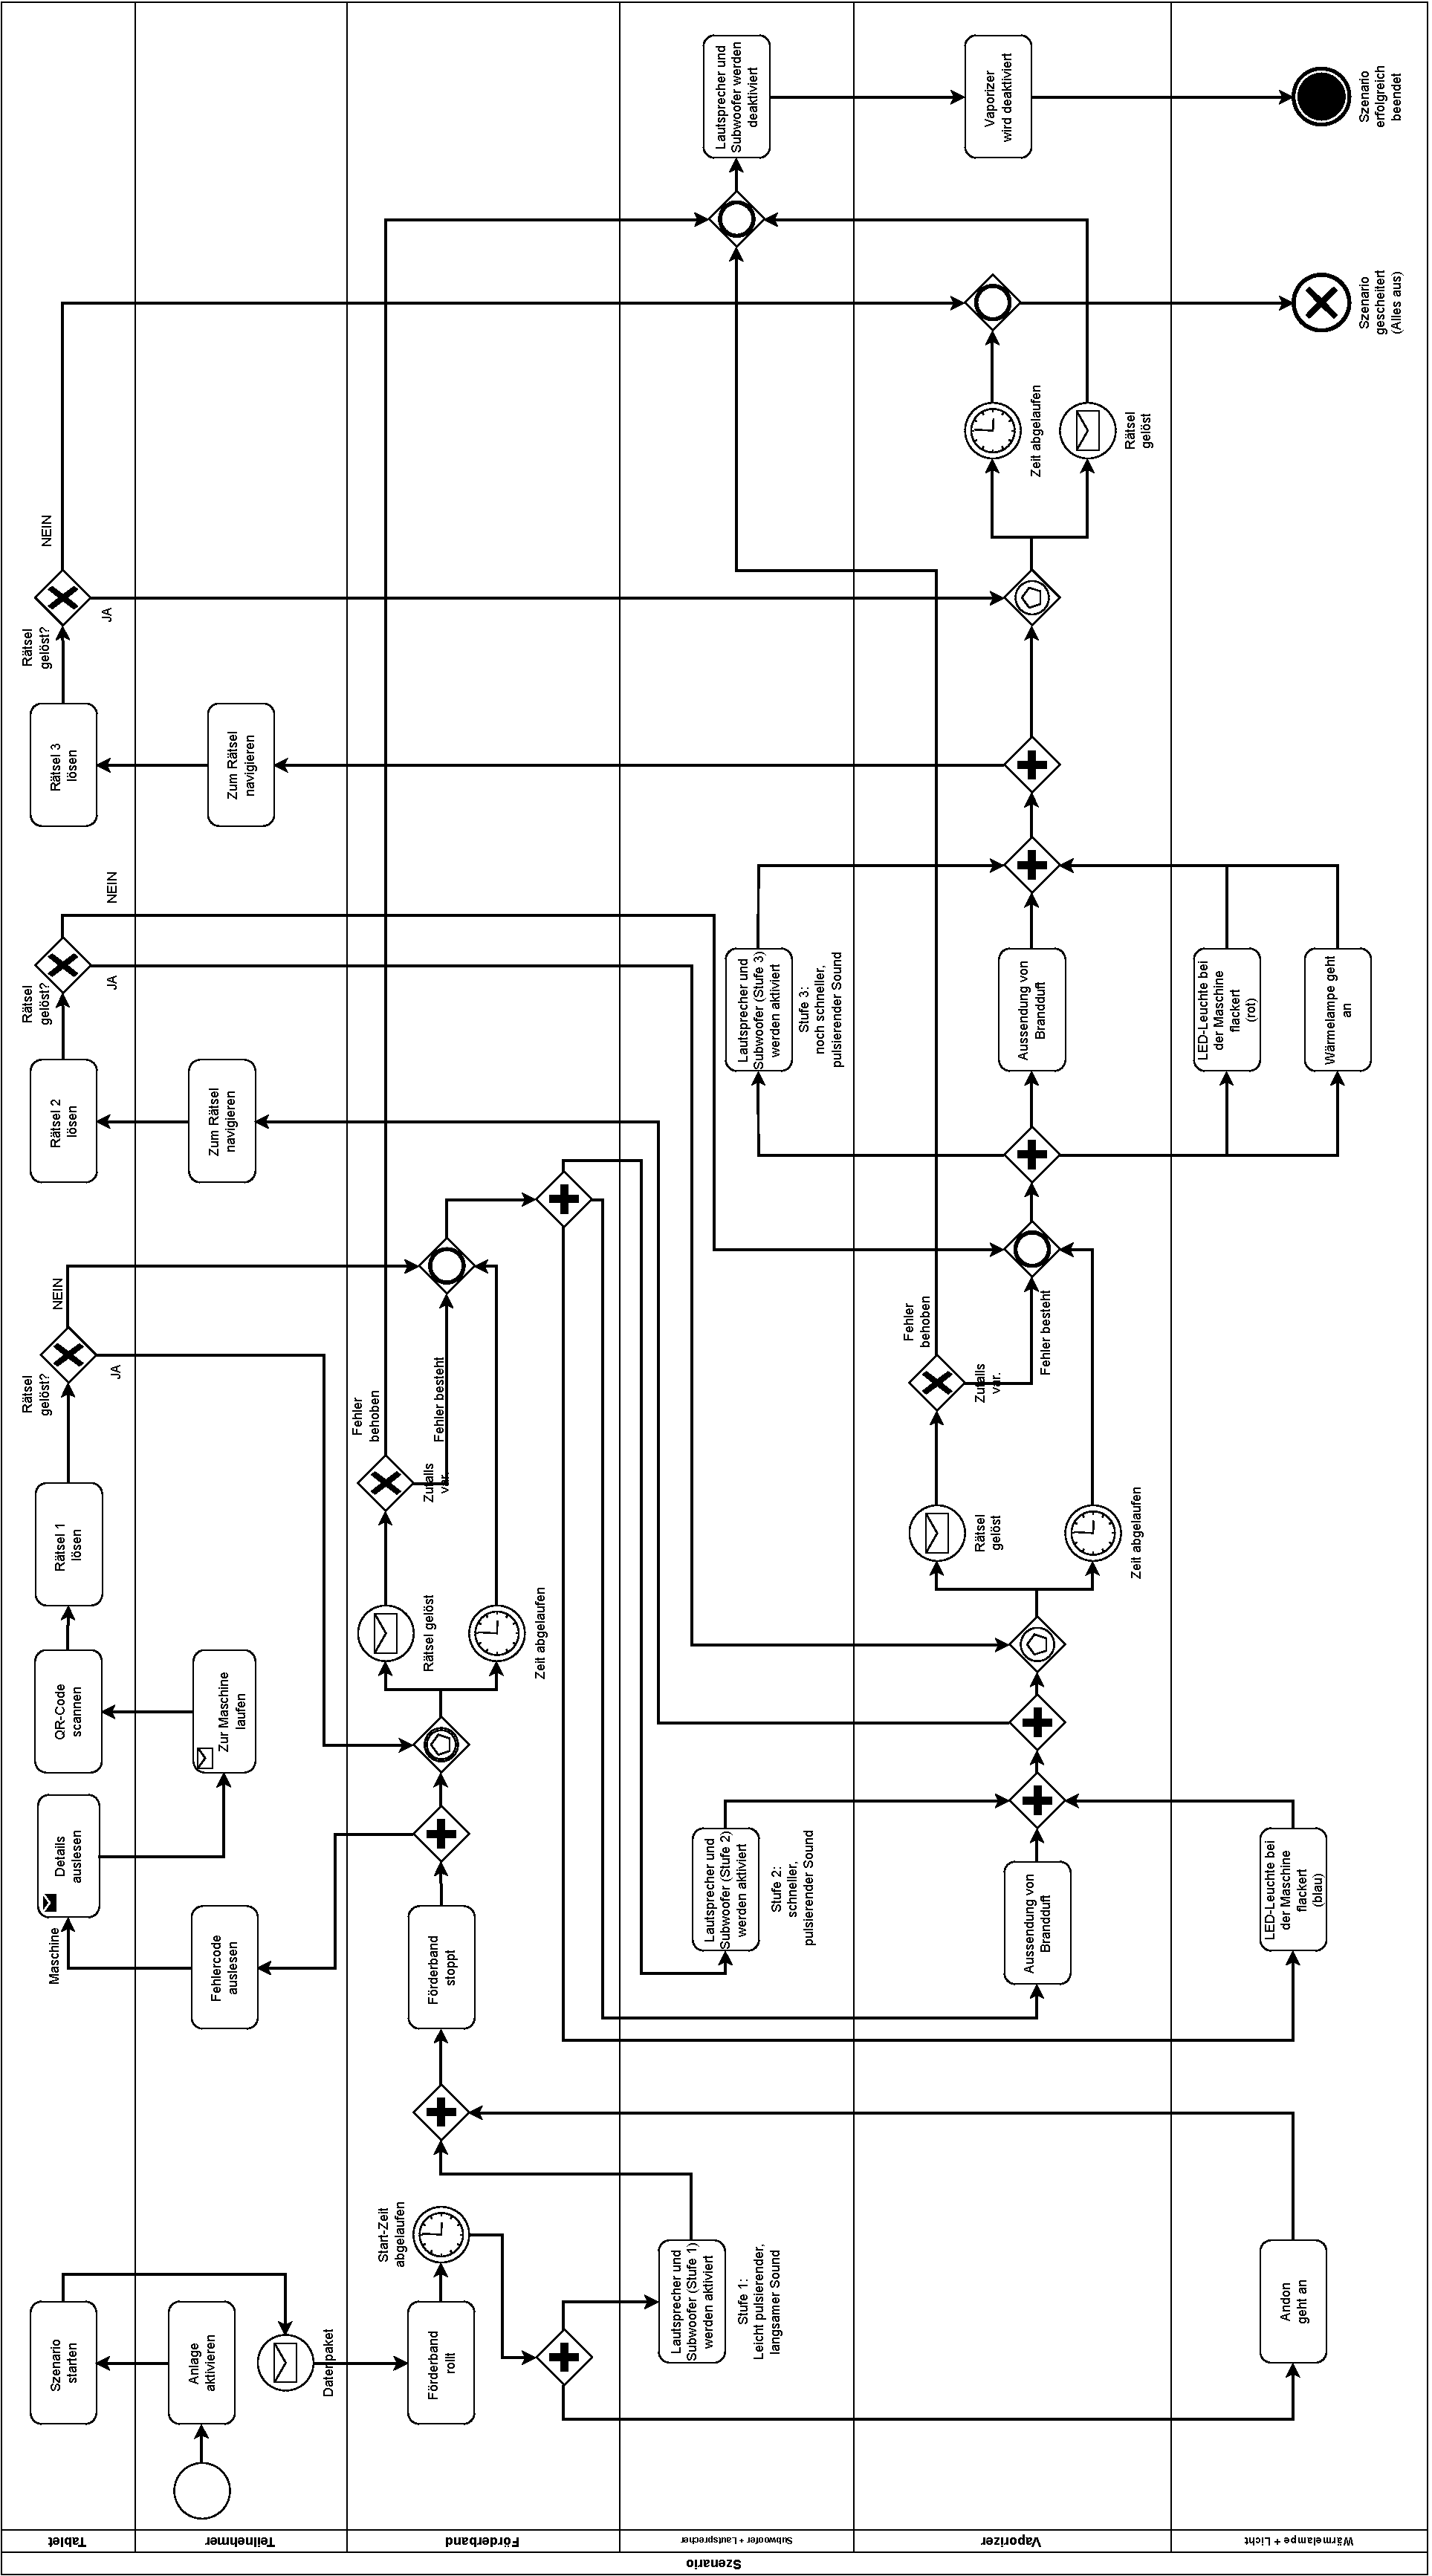
\includegraphics[pages=1, scale=0.4]{res/Finales Szenario BPMN(korrigiert).drawio-5.pdf}
%(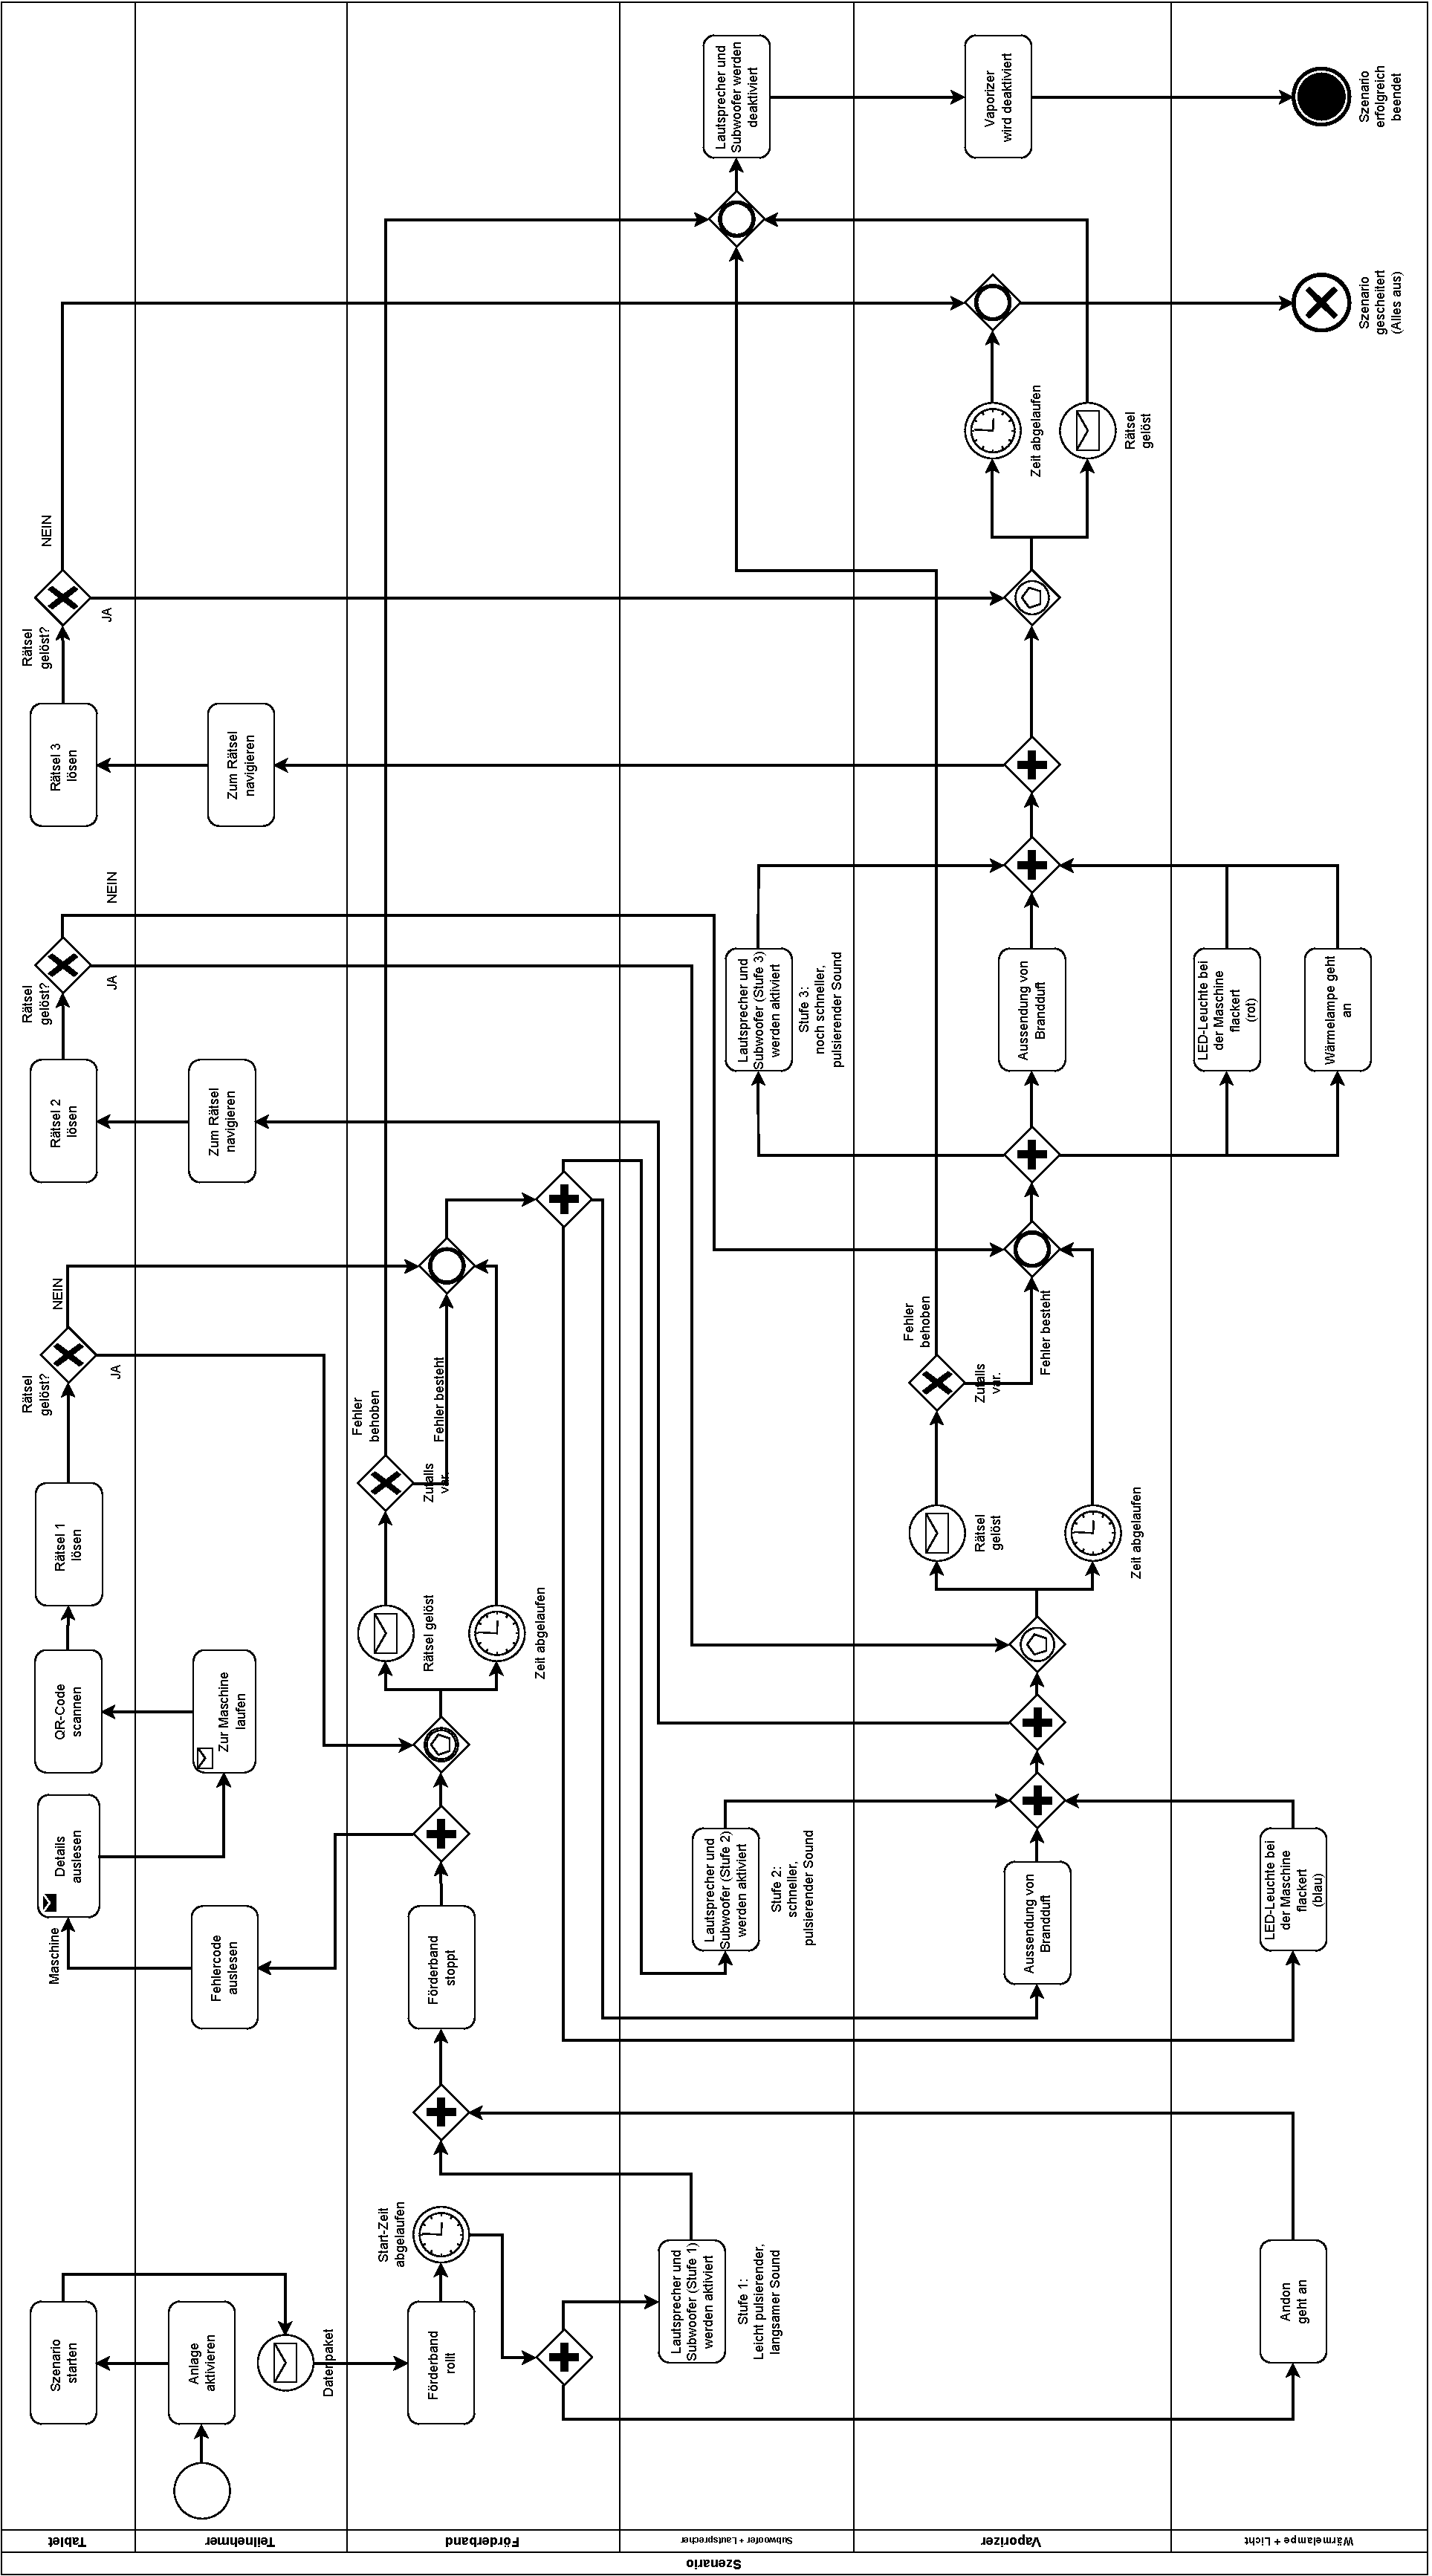
\includegraphics[pages=1, scale=0.45]{res/Finales Szenario BPMN(korrigiert).drawio-5.pdf})

\section{Ausarbeitung des Alarmszenarios}

In dem nun folgenden Kapitel werden die Ergebnisse der Ausarbeitung vorgestellt. Zunächst werden wiederkehrende Begriffsdefinitionen geboten, um Kernelemente des Alarmszenarios zu spezifizieren und voneinander abzugrenzen. Anschließend wird der grundlegende Ablauf des MVPs erläutert.

\subsection{Begriffsabgrenzung}

Die nachfolgenden Begriffe stellen zentrale Elemente dar, welche im Kontext der Alarmsimulation zusammenwirken:

\begin{description}
    \item [\textbf{Übungsteilnehmer:}] 
     Person, welche die Alarmsimulation an einer angebundenen Industrie 4.0 Simulationsanlage durchläuft und Versuche unternimmt, die simulierte Störung in kürzester Zeit zu beheben. 

     \item [\textbf{Übungsleiter:}] 
    Person, welche die Administration der Alarmsimulation verantwortet und Szenarioart, als auch Zeitdauer von Eskalationsstufen individuell konfiguriert.

    \item [\textbf{Immersionsobjekt:}] 
   Objekt, welches nach Adressierung durch die Ablauflogik übermittelte Immersionseffekte durchführt. Dieses Objekt, beispielsweise ein Lautsprecher, kann etwa Brandgeräusche emittieren und sorgt für eine stärkere Immersion der Simulation auf den Übungsteilnehmer.

   \item [\textbf{Simulationstablett:}] 
   Zentrales Steuerungs- und Kommunikationselement für den Übungsteilnehmer, um die Entstörung durch Eingaben auf Tablet zu realisieren.

    \item [\textbf{Entstörungsvorgang:}] 
    Phase in der Ablauflogik, in der durch den Übungsteilnehmer versucht wird, die Störung durch das Lösen eines szenarionahen Rätels zu beheben. Der Entstörungsvorgang kann dabei erfolgreich, als auch unerfolgreich verlaufen.
   
   \item [\textbf{Eskalationsstufe:}] 
   Phase in der Simulation eines Szenarios, in welcher eine bestimmte Ausprägung von Immersionseffekten als auch Störungsbild gegeben ist. Eine Eskalationsstufe steht dabei in einer Rangfolge beziehungsweise Stufe zu anderen Eskalationsstufen, um eine Verstärkung des Immersionseffektes im Zeitverlauf der Simulation zu realisieren.
\end{description}

\subsection{Szenario}

Als \textit{MVP} Szenario wurde sich für die Simulation des Brandes einer Maschine im Kontext des \textit{Zentrums Industrie 4.0} entschieden. In den anschließenden Unterabschnitten wird beginnend der Ablauf des \textit{MVP} Szenarios skizziert und die einzelnen Eskalationsstufen dargelegt. Darauf folgend werden zusammengehörige Entstörungsvorgänge erläutert und ein Einblick in die Administration der Alarmszenarien geboten. Abschließend werden Begleitdokumente zur Unterstützung der Übungsteilnehmer und des Übungsleiters vorgestellt und ein Gesamtüberblick mithilfe eines aufgestellten Prozessmodells (siehe Kapitel \ref{chap:process model}) geboten.

\subsubsection{Ablauf}

Vor Start der Simulation des MVPs \textit{Maschinenbrand} ist durch den Übungsleiter sicherzustellen, dass die Anlage im \textit{Zentrum Industrie 4.0} aktiviert ist. Auf dem Tablet in der Administrationsoberfläche des Übungsleiters ist der Button \textit{Szenario starten} zu klicken, um das Szenario für den Übungsteilnehmer zu starten. In folgender Abbildung ist die Startoberfläche eines Übungsteilnehmers zu sehen:

\begin{figure}[h]
    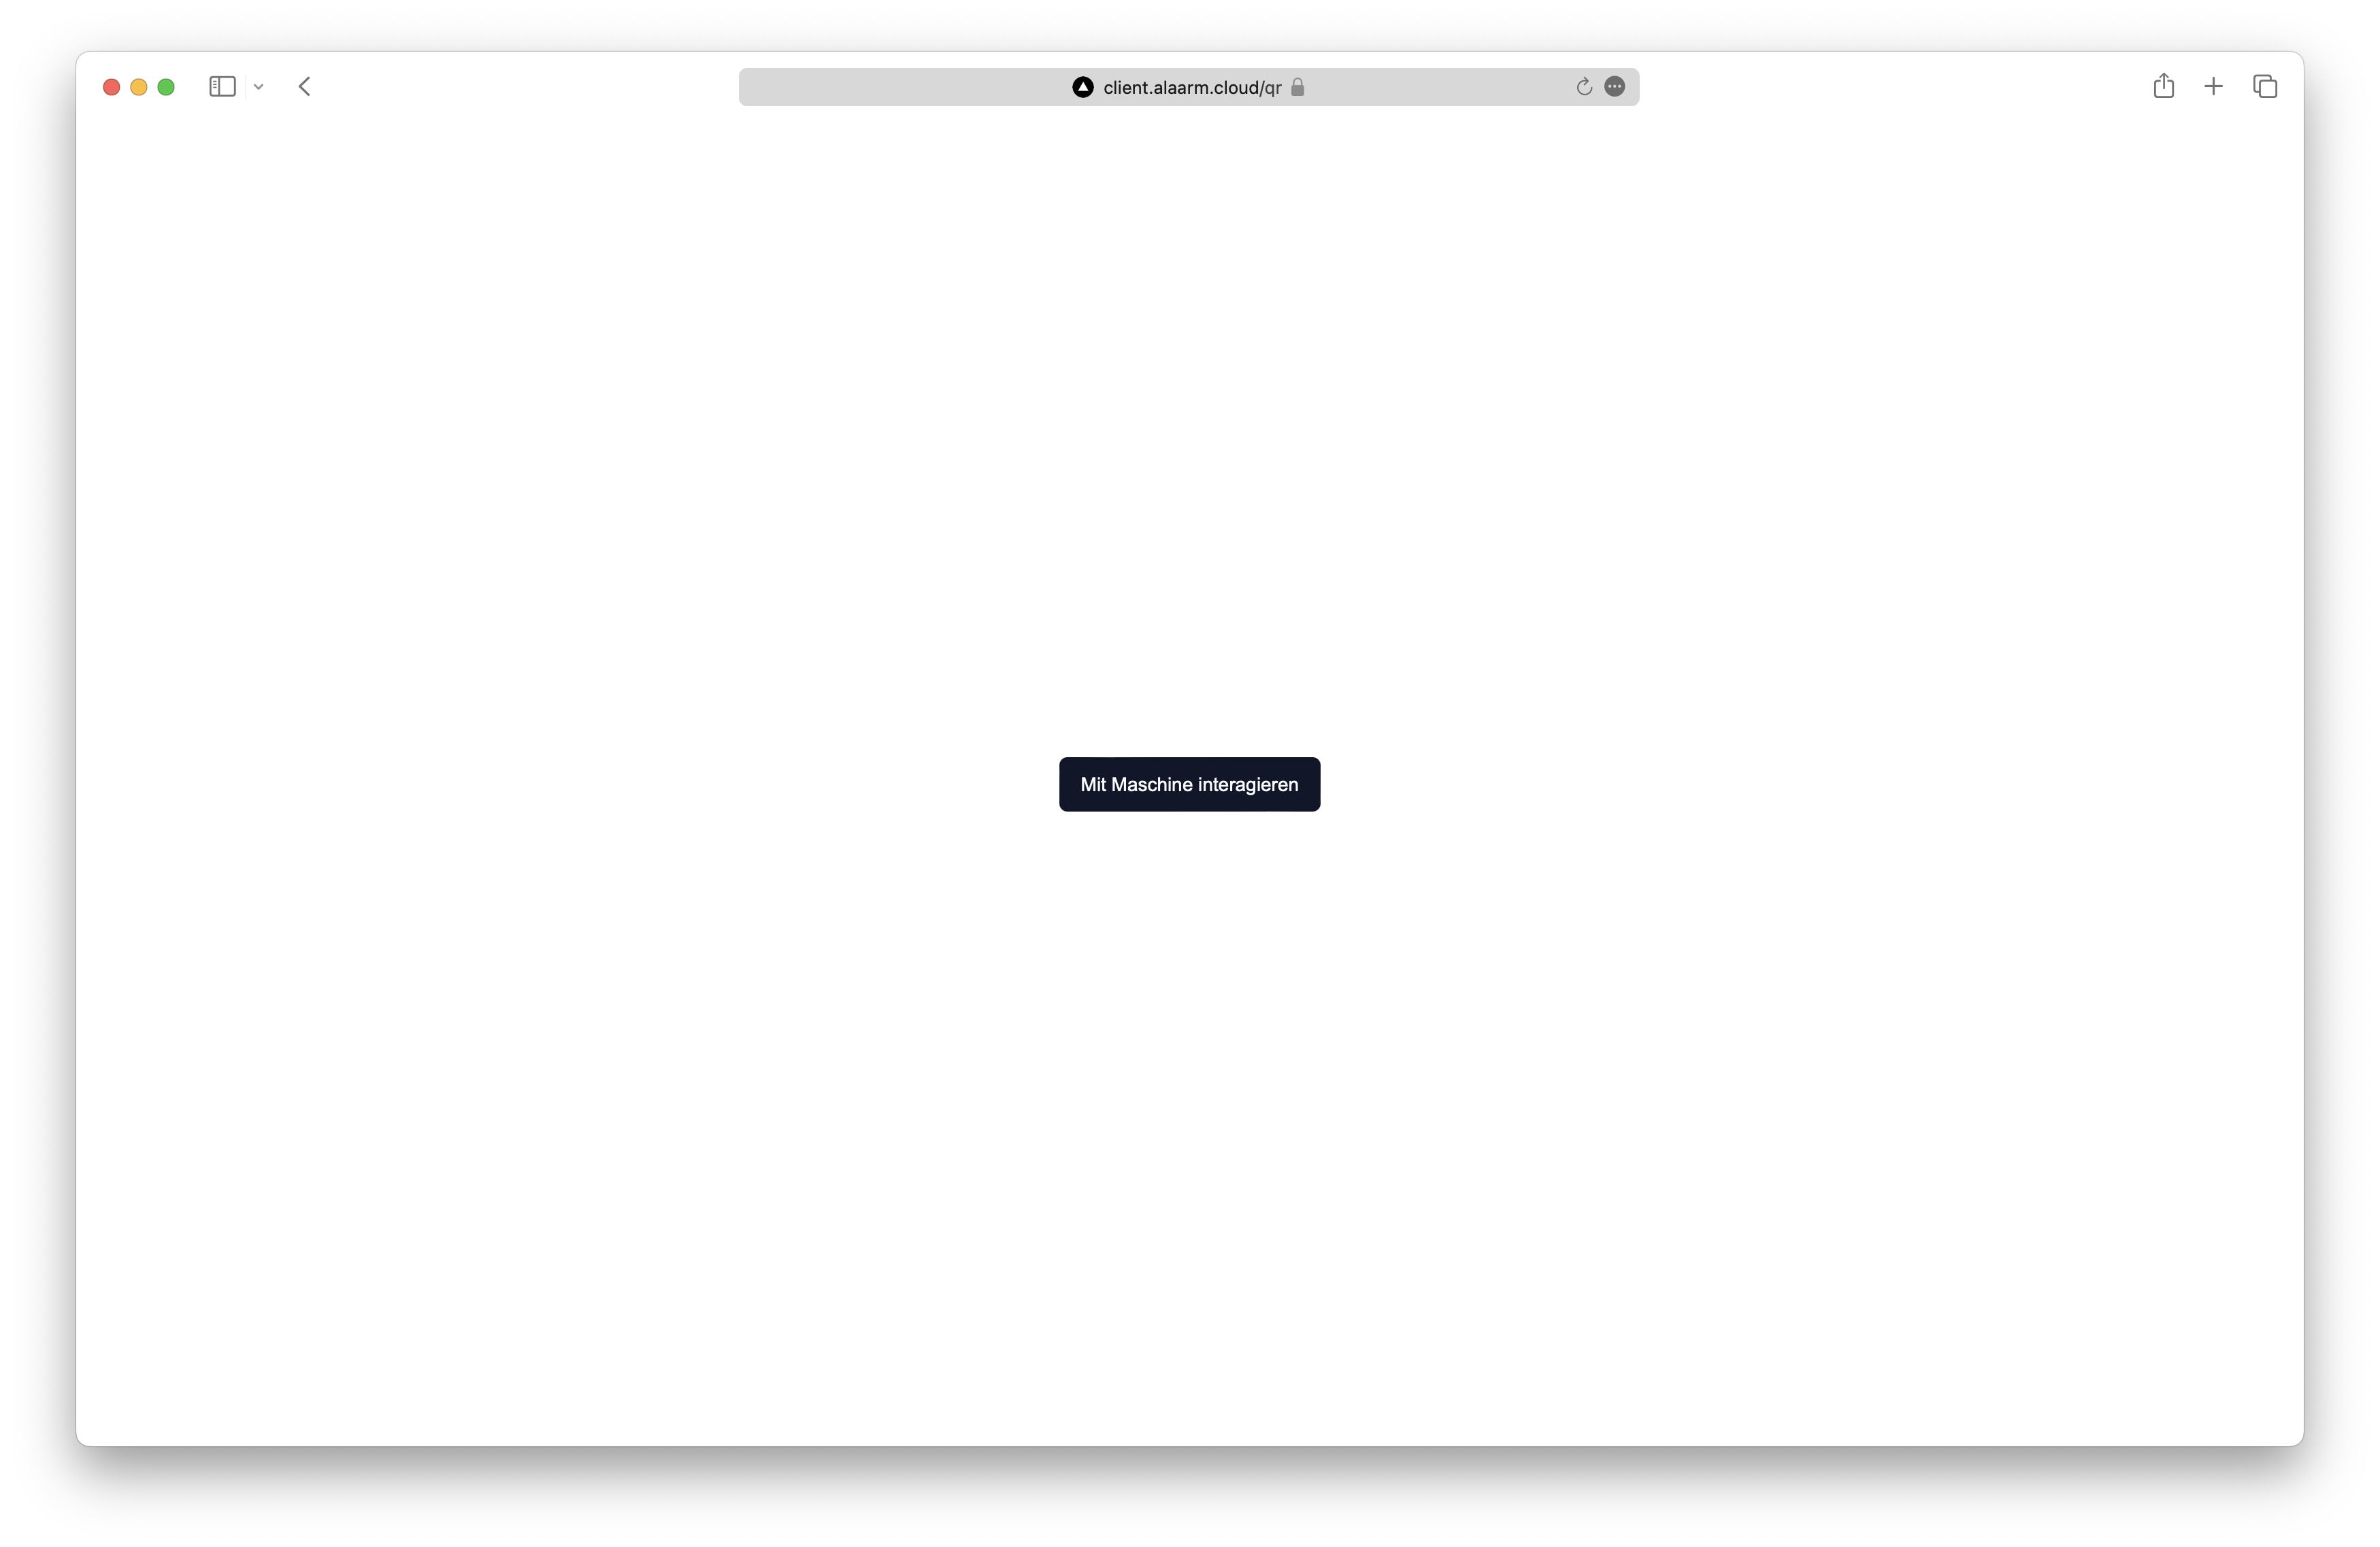
\includegraphics[width=15cm, height=9.61cm]{res/web_interface.png}
    \centering
   \caption{Web Interface}
\end{figure}

Mit der Betätigung des Buttons rollen die Förderbänder der Anlage an. 
Nach Ablauf der konfigurierten Startzeit wird die Eskalationsstufe 1 des Szenarios \textit{Maschinenbrand} ausgelöst. Entsprechende Immersionseffekte werden ausgelöst und die Förderbänder werden gestoppt.

In diesem Moment beginnt für den Übungsteilnehmer der konfigurierte Zeitraum, in dem die aufgetretene Störung zwingend zu lösen ist. Auf der Simulationsoberfläche des Simulationstabletts vom Übungsteilnehmer erscheint ein Fehlercode. Der  Information kann die Person entnehmen, zur welcher Maschine mit dem Störungsbild Brand zu navigieren ist. Auf dem Bildschirm der Maschine ist ein QR-Code eingeblendet, welcher durch den Scanner der Simulationsoberfläche des Simulationstabletts durch den Übungsteilnehmer einzuscannen ist. In der nachfolgenden Abbildung ist die Funktionsweise und der Aufbau des QR Scanners exemplarisch dargestellt:

\begin{figure}[h]
   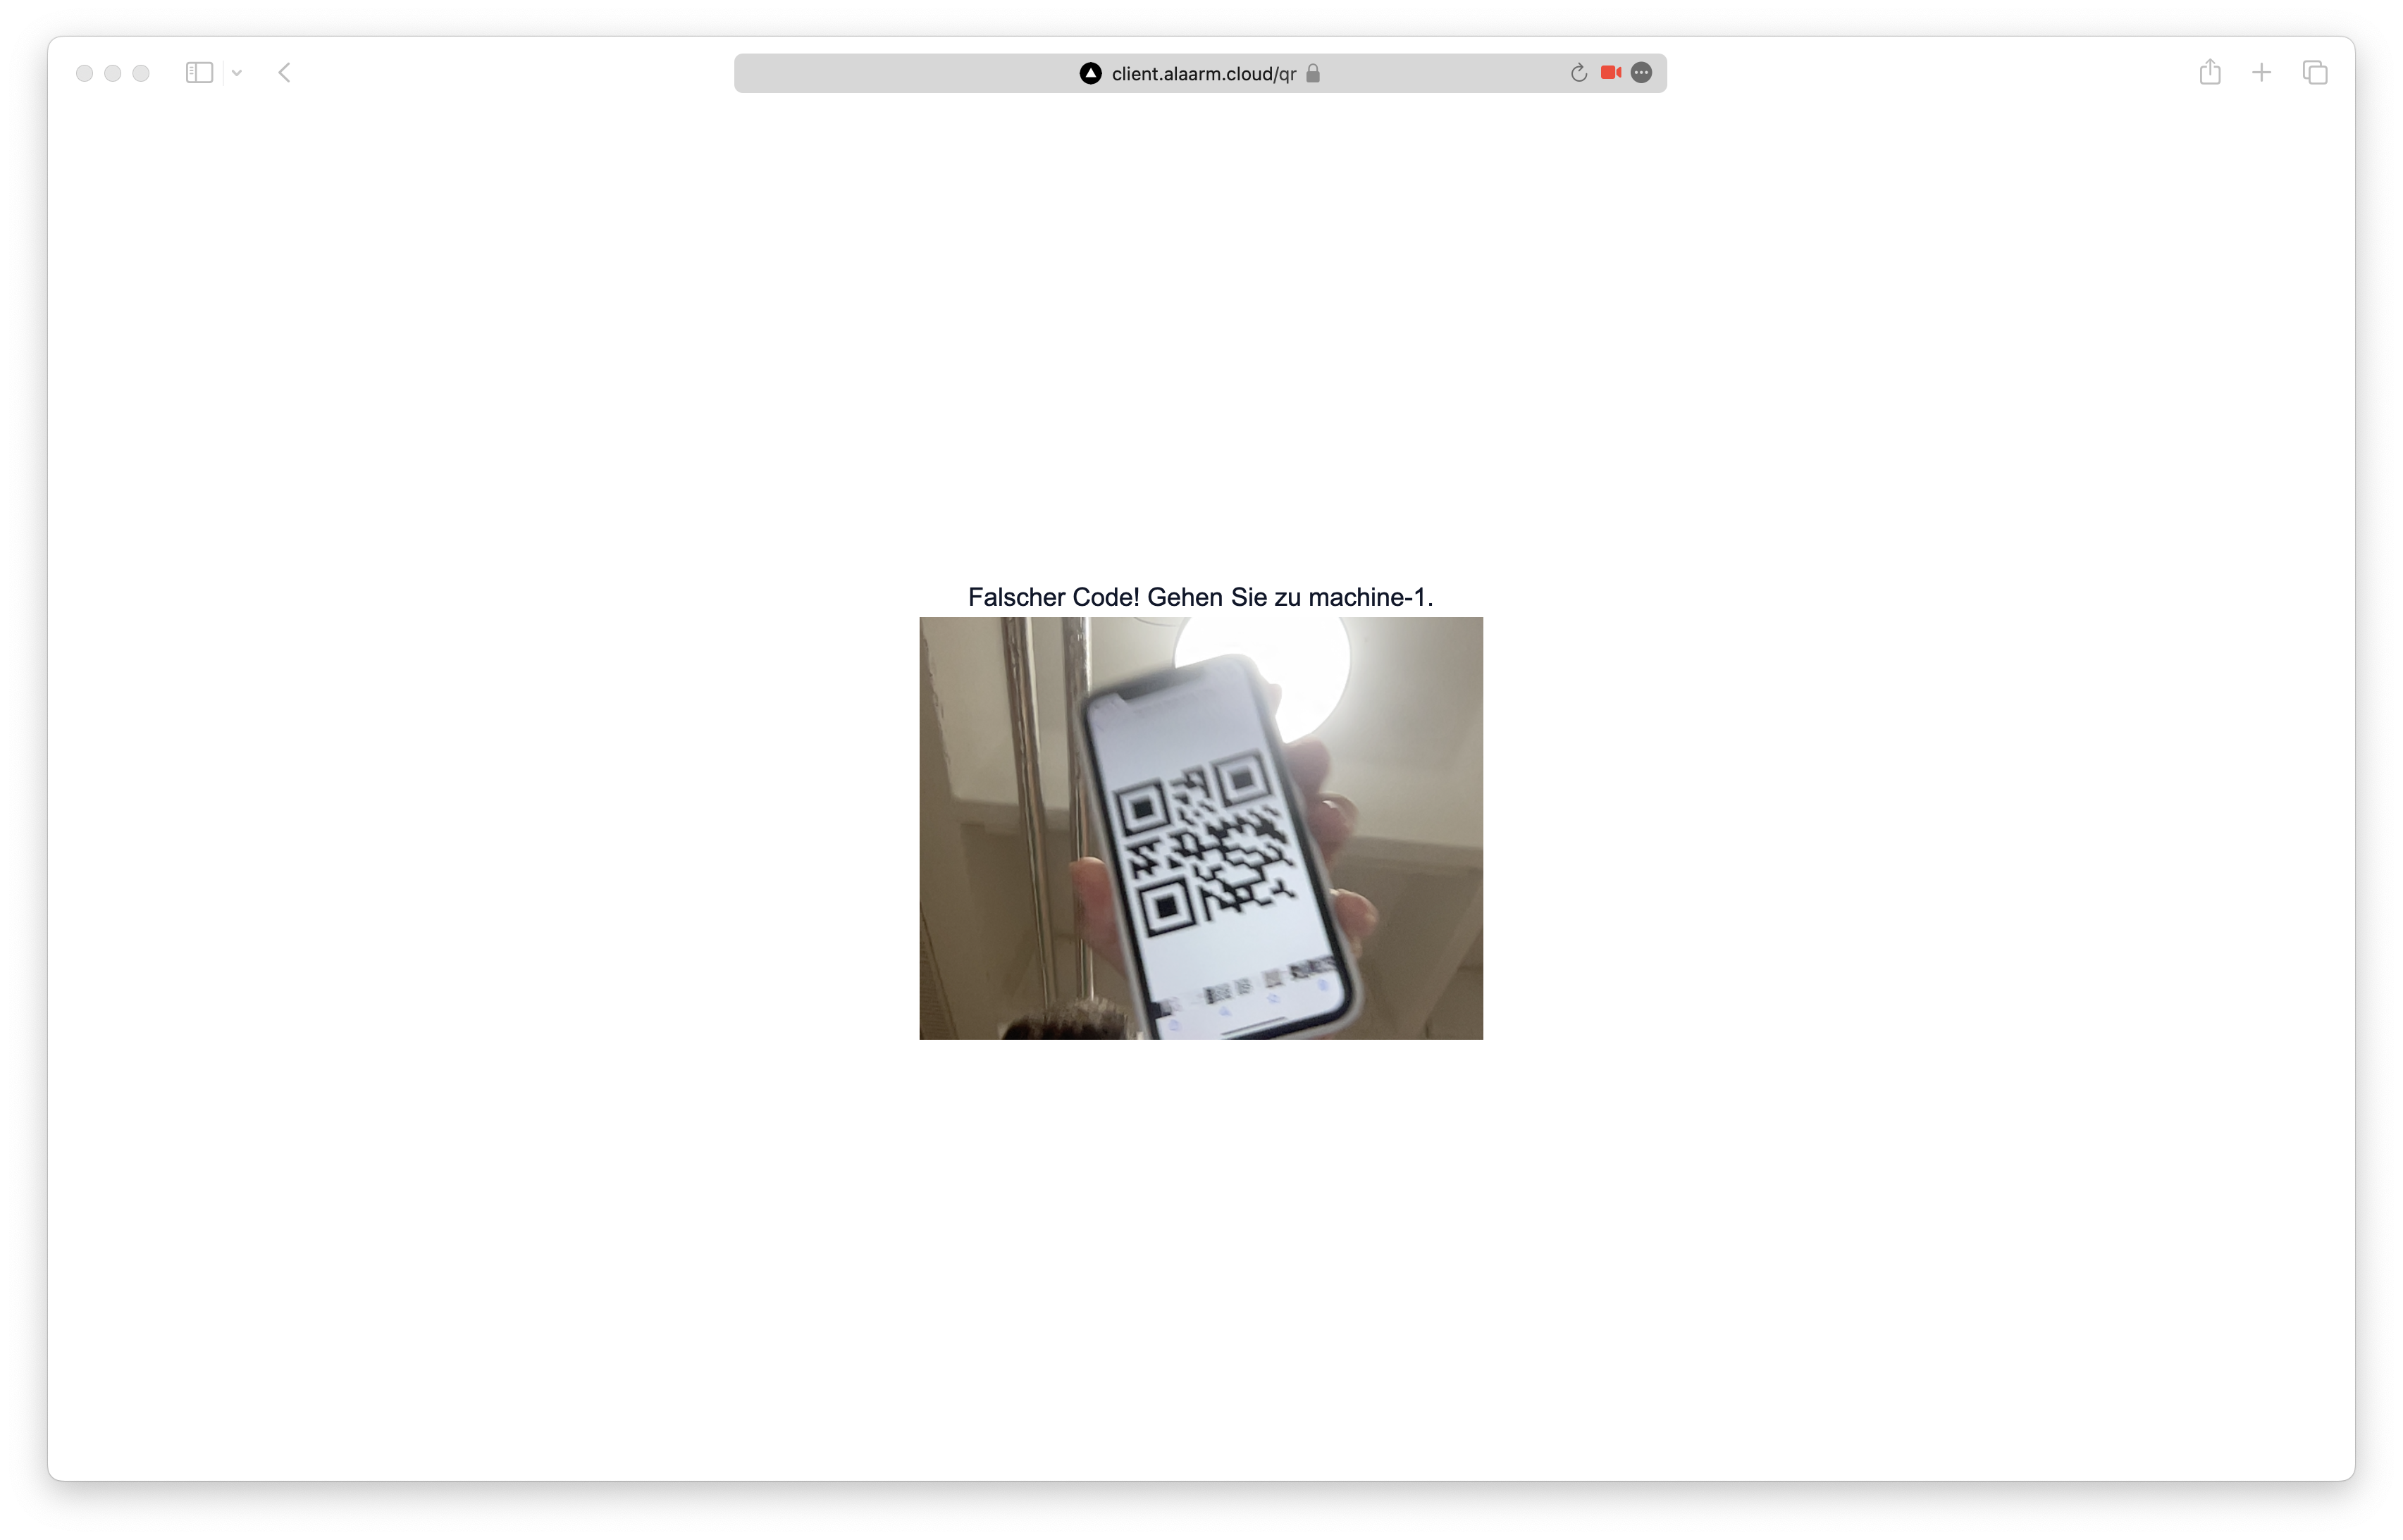
\includegraphics[width=15cm, height=9.61cm]{res/qr_code_scanner.png}
   \caption{QR-Code Scanner}
\end{figure}

Mit dem erfolgreichen Scan beginnt der eigentliche Entstörungsvorgang, für den dem Übungsteilnehmer ein Rätsel zur Entstörung eingeblendet wird. Der Beschreibung des Rätsels ist die Aufgaben zu entnehmen, die der Übungsteilnehmer nun zu lösen hat. Jedes Rätsel zur Entstörung bildet drei Ausgangsszenarien. Sofern das Rätsel falsch gelöst wurde, wird entweder, sofern vorhanden, die nächste Eskalationsstufe mit zusammenhängendem Entstörungsvorgang eingeleitet. Sofern keine weitere Eskalationstufen vorhanden sind, gilt das Alarmszenario für den Übungsteilnehmer als gescheitert. Die zweite Ausgangsmöglichkeit ist die erfolgreiche Lösung des Rätsels zur Entstörung, wobei aufgrund einer durch den Übungsleiter anpassbaren Zufallsvariable bestimmt wird, ob der Entstörungsversuch wirklich erfolgreich war. Sofern die Zufallsvariable für den Übungsteilnehmer ungünstig ist, ist entsprechende Lösung nicht ausreichend für die Behebung und ggf. wird eine weitere Eskalationsstufe eingeleitet. Sofern die Zufallsvariable sich nicht der erfolgreichen Lösung des Entstörungsvorgangs entgegenstellt, ist ein erfolgreicher Entstörungsversuch und damit eine erfolgreiche Beendigung des Alarmszenarios nur gegeben, wenn der Zeitraum zur Lösung der Entstörung eingehalten wurde. Ist dies nicht der Fall, werden bei Verfügbarkeit weitere Eskalationsstufen eingeleitet oder das Szenario gilt auch hier als gescheitert.  

\subsubsection{Eskalationsstufen}

Das realisierte Szenario \textit{Maschinenbrand} verfügt über insgesamt drei Eskalationsstufen.

Bei der \textbf{ersten Eskalationsstufe} werden als Immersionsobjekte der Lautsprecher, Subwoofer und die Andon-Signalleuchte adressiert. Vom Lautsprecher und Subwoofer wird ein leiser, langsamer und leicht pulsierender Sound des Knackens und Rauschens abgespielt. Gleichzeitig schaltet sich die rote Lampe der Andon-Lampe an, um eine Störung der Maschine zu signalisieren.

Im Rahmen der \textbf{zweiten Eskalationsstufe} wird durch die Lautsprecher und den Subwoofer ein schnellerer, stärker pulsierender Sound mit ähnlichen Geräuschen abgespielt. Zusätzlich wird Brandduft über einen Vaporizer ausgesondert und eine LED innerhalb der Maschine fängt an mit blauem Licht zu flackern. 

Bei der letzten, \textbf{dritten Eskalationsstufe} des \textit{MVP} Szenarios beschleunigt sich der Sound des Brandgeräusches, der durch den Lautsprecher und Subwoofer abgespielt wird. Dazu wird verstärkt Brandgeruch und Rauch durch den Vaporizer ausgesondert. Der LED-Streifen in der Maschine beginnt nun rot zu flackern, um Flammen zu imitieren. Zusätzlich wird eine Wärmelampe angesteuert, welche zur Emittierung von Wärme aktiviert wird.

Durch den stufenbasierten Aktivierungslauf, sofern der Entstörungsvorgang nicht erfolgreich durch den Übungsteilnehmer absolviert wird, kann die immersive Wahrnehmung des Alarmszenarios des Übungsteilnehmers im Zeitverlauf gesteigert werden. Mithilfe der gewählten Konfiguration kann ein reales Szenario des Maschinenbrandes und die Effekte auf Maschinenführer simuliert werden. Die Ablauflogik kann als Überblick im Kapitel \ref{chap:process model} visuell nachvollzogen werden.

\subsubsection{Entstörungsvorgänge}

An jede aktivierte Eskalationsstufe schließt ein individueller Entstörungsvorgang an. Der Übungsteilnehmer bekommt bei Auslösung einer Eskalationsstufe einen Fehlercode übergeben, auf Basis dessen Informationen die richtige Maschine anzulaufen ist. Via Scan des QR-Codes an der Maschine wird die Oberfläche zur Entstörung aufgerufen. Je nach Eskalationsstufe im \textit{MVP}-Szenario wird eines von insgesamt drei Rätseln aufgerufen.

Der \textbf{erste Entstörungsvorgang} des MVPs gibt dem Übungsteilnehmer den Hinweis, dass aufgrund des \textit{Fehlers E5432} der Betriebsablauf der Anlage im \textit{Zentrum Industrie 4.0} gestört ist. Um die Reihenfolge an Werkschritten wiederherzustellen, müssen auf der Weboberfläche des Tablets des Endnutzers die Nummern 1 bis 10 in aufsteigender Reihenfolge angewählt werden. Initial ist eine Zeitbegrenzung von 10 Sekunden vorgesehen. Die Strukturierung von Rätseln kann anhand der nachfolgenden Abbildungen nachvollzogen werden.

\begin{figure}[H]
   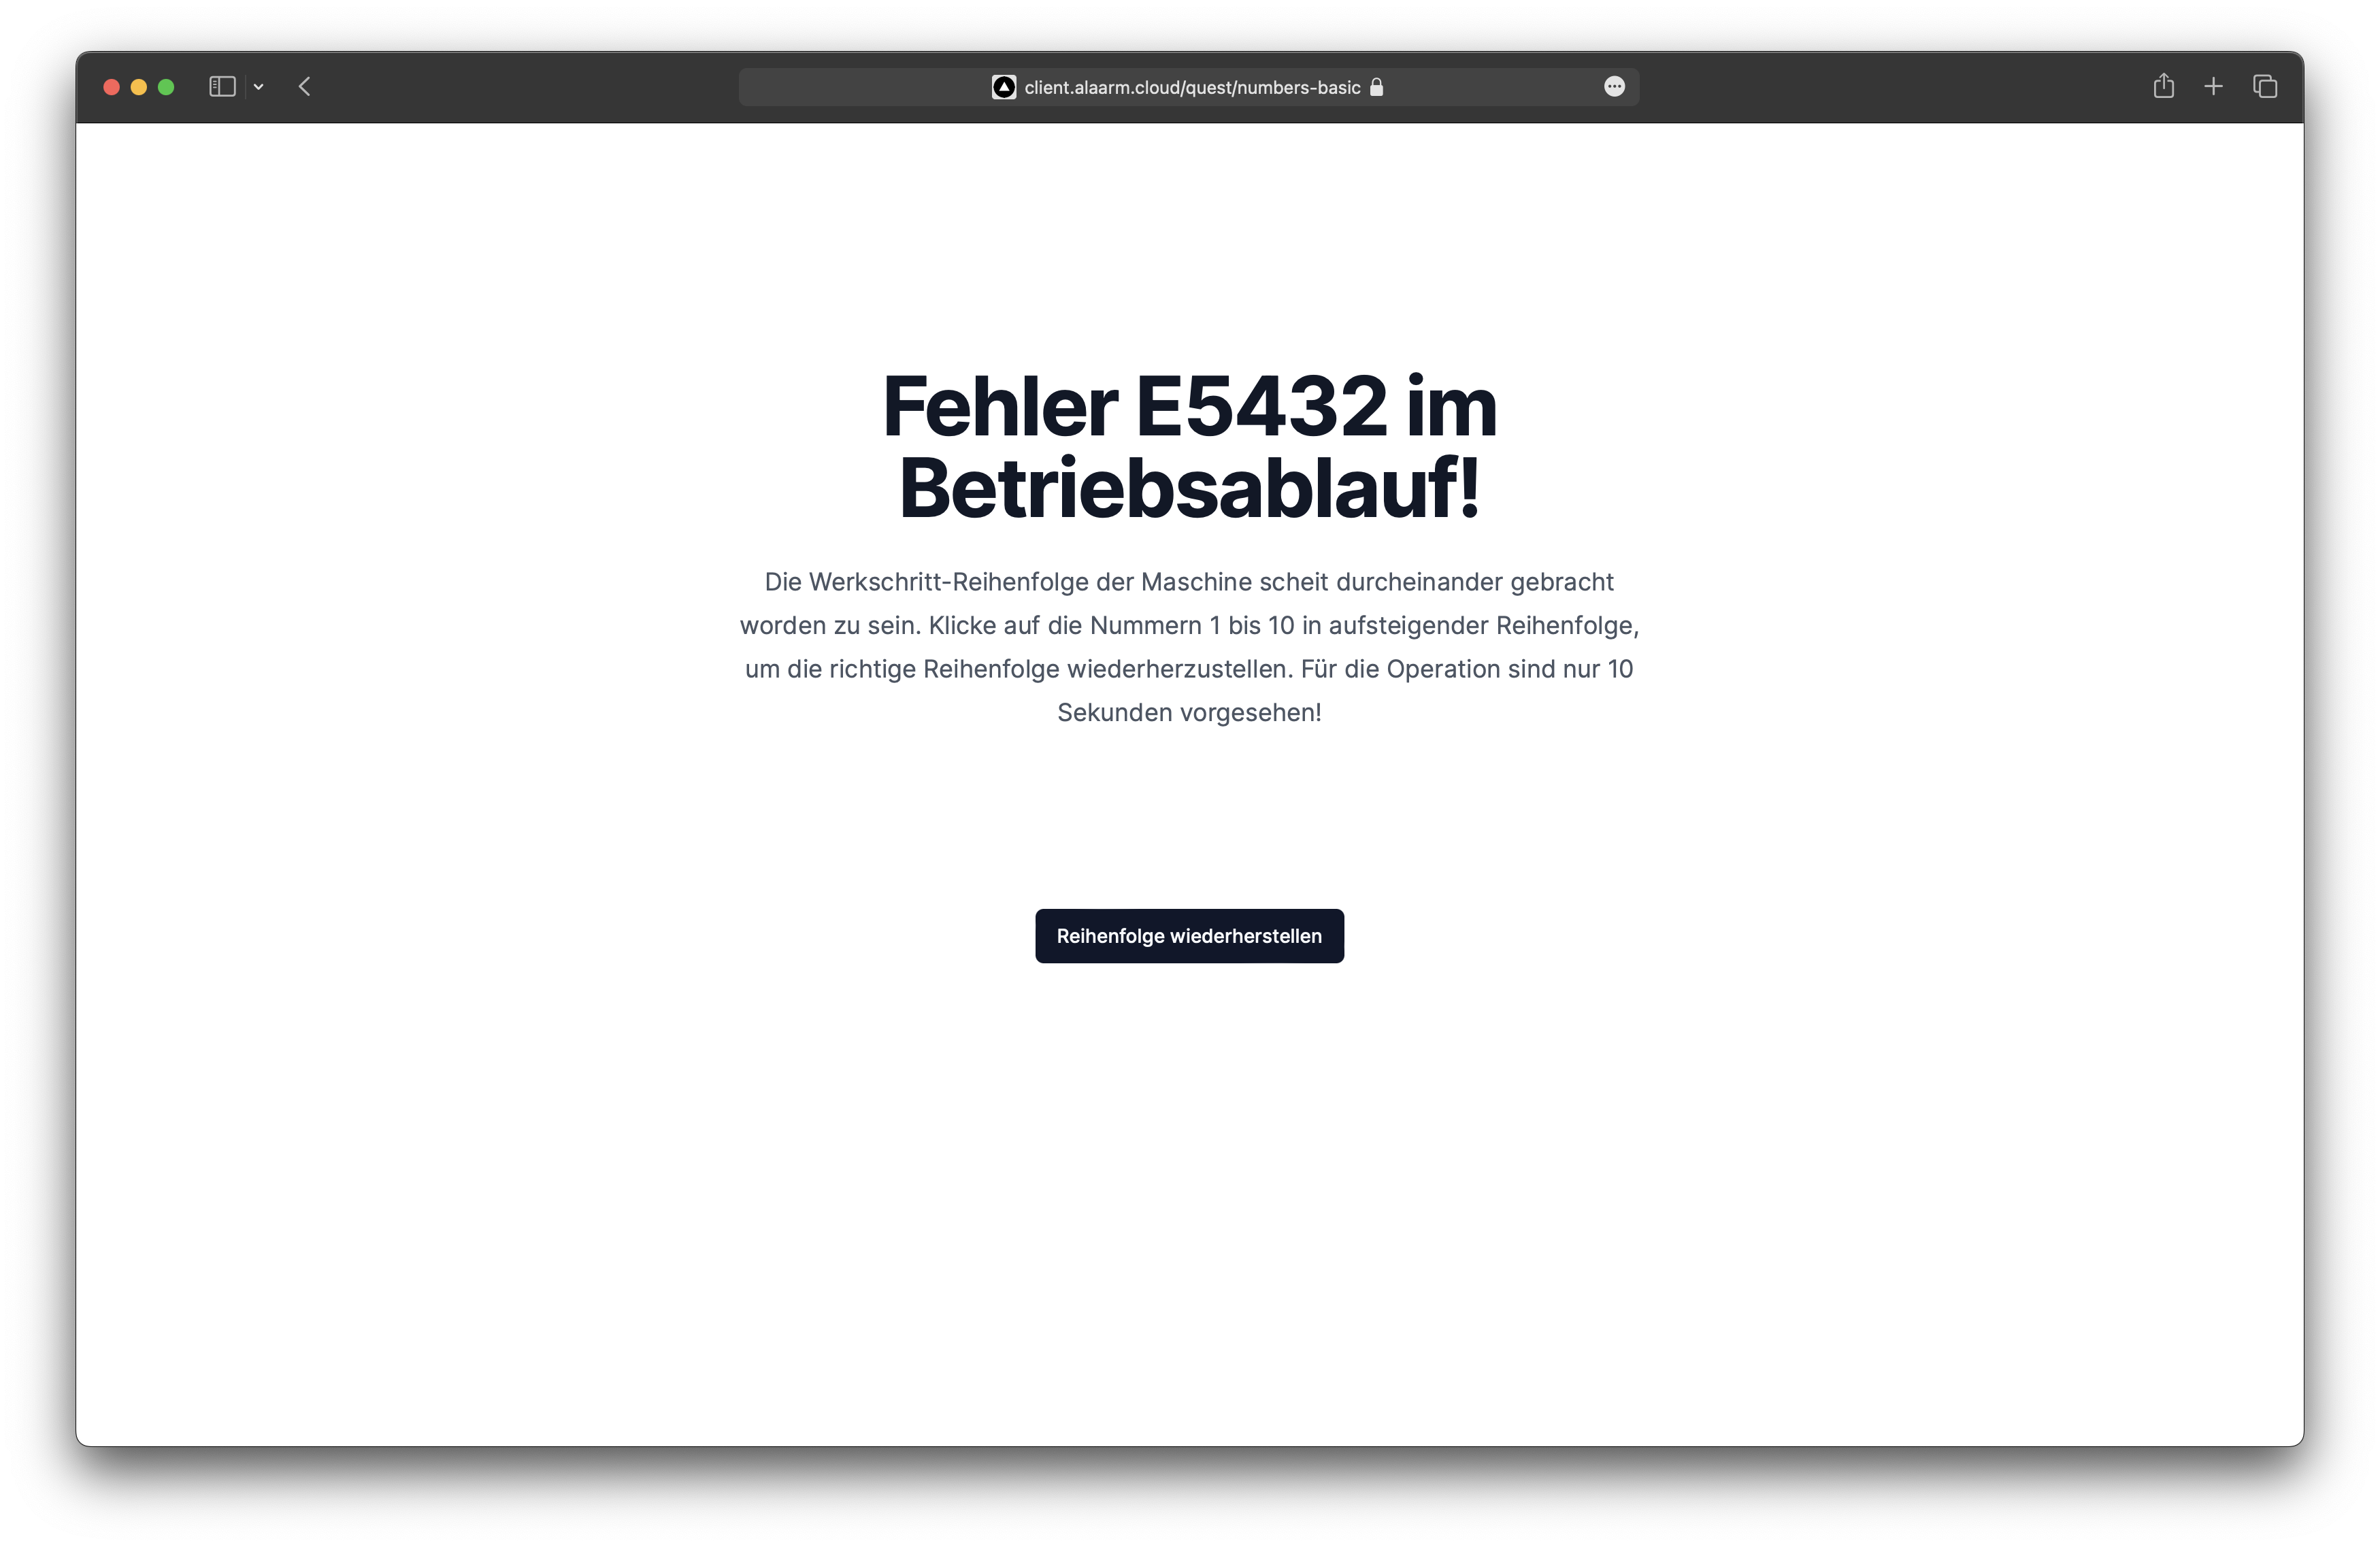
\includegraphics[width=15cm, height=9.61cm]{res/quest_01_v2.png}
   \caption{Hinweisseite - Rätsel 1}
\end{figure}

\begin{figure}[H]
   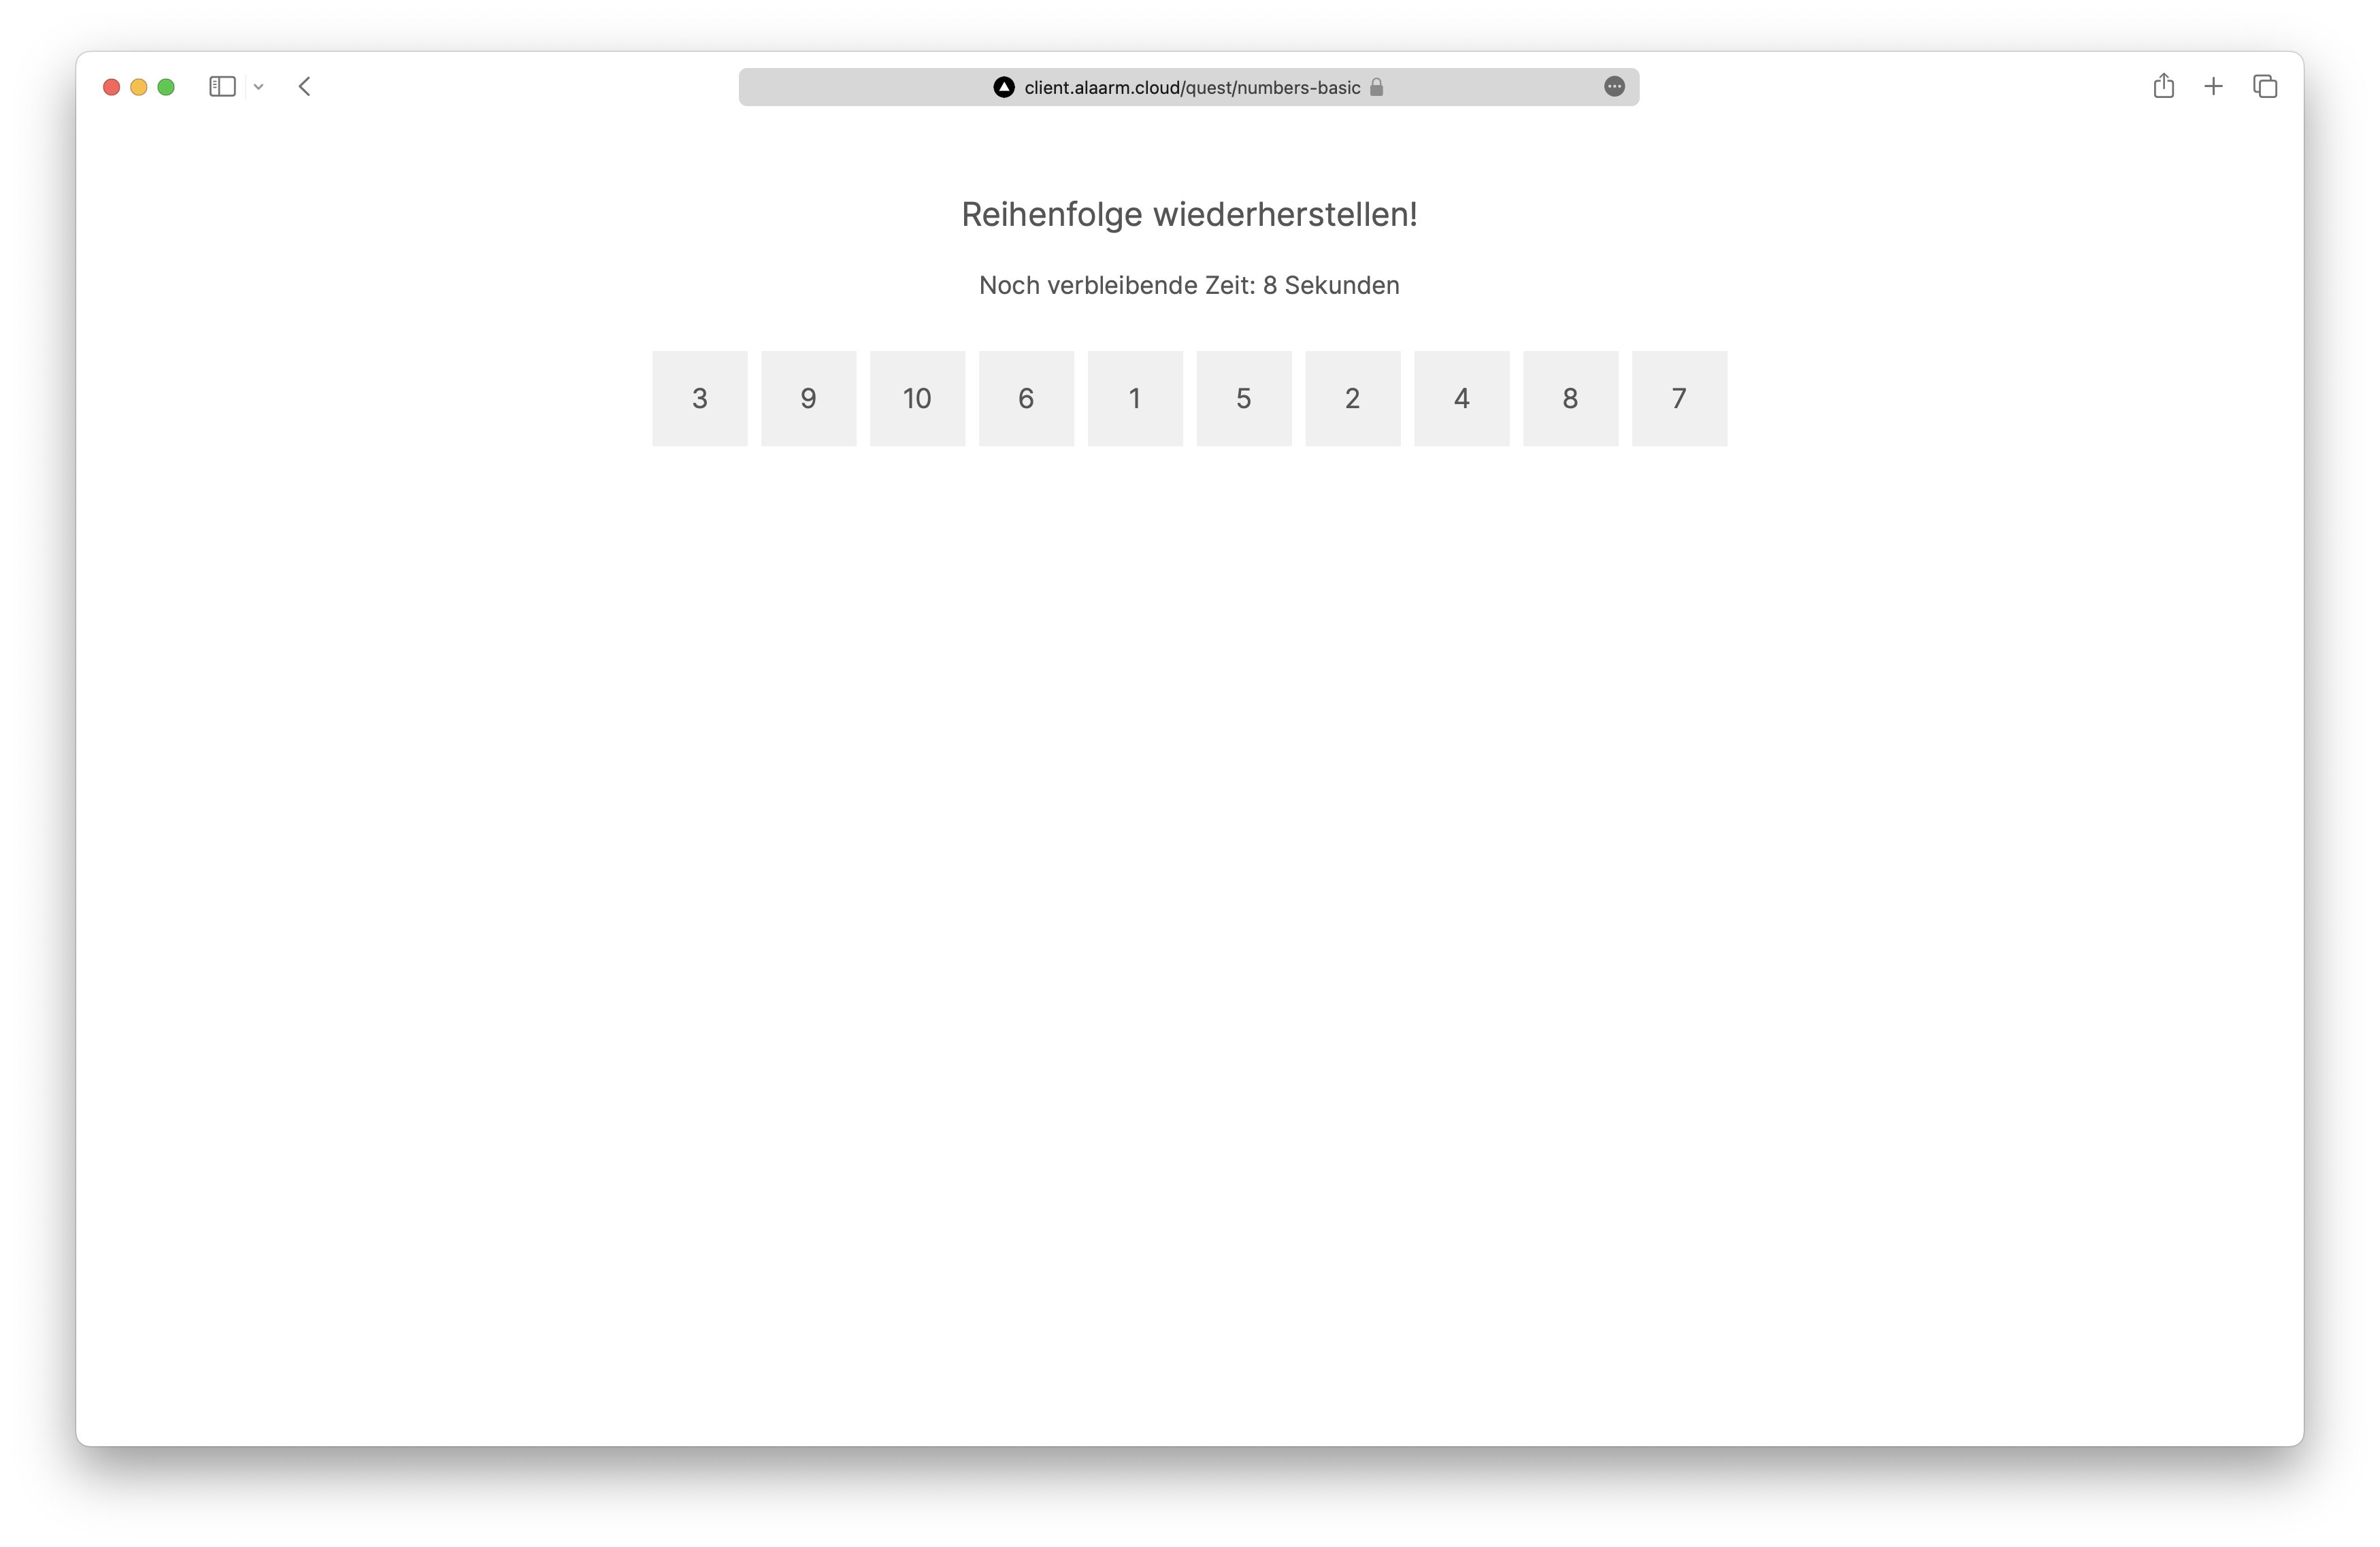
\includegraphics[width=15cm, height=9.61cm]{res/quest_01.png}
   \caption{Rätsel 1}
\end{figure}

Sofern es zum \textbf{zweiten Entstörungsvorgang} kommt, ist ein Rätsel mit dem Störungsbild \textit{P4222 - Störung des Produktionsprozesses} zu lösen. Hier ist eine Störung im Prozessfluss der Maschine gegeben, wodurch es zur Alarmlage der Überhitzung kommt. Auch hier müssen Prozesse in die richtige Reihenfolge gebracht werden, wobei die Prozessschritte durch eine Neukalibrierung nach 5 und 10 Sekunden neu gemischt werden. Die graphische Realisierung kann der nachgelagerten Grafik entnommen werden:

\begin{figure}[H]
   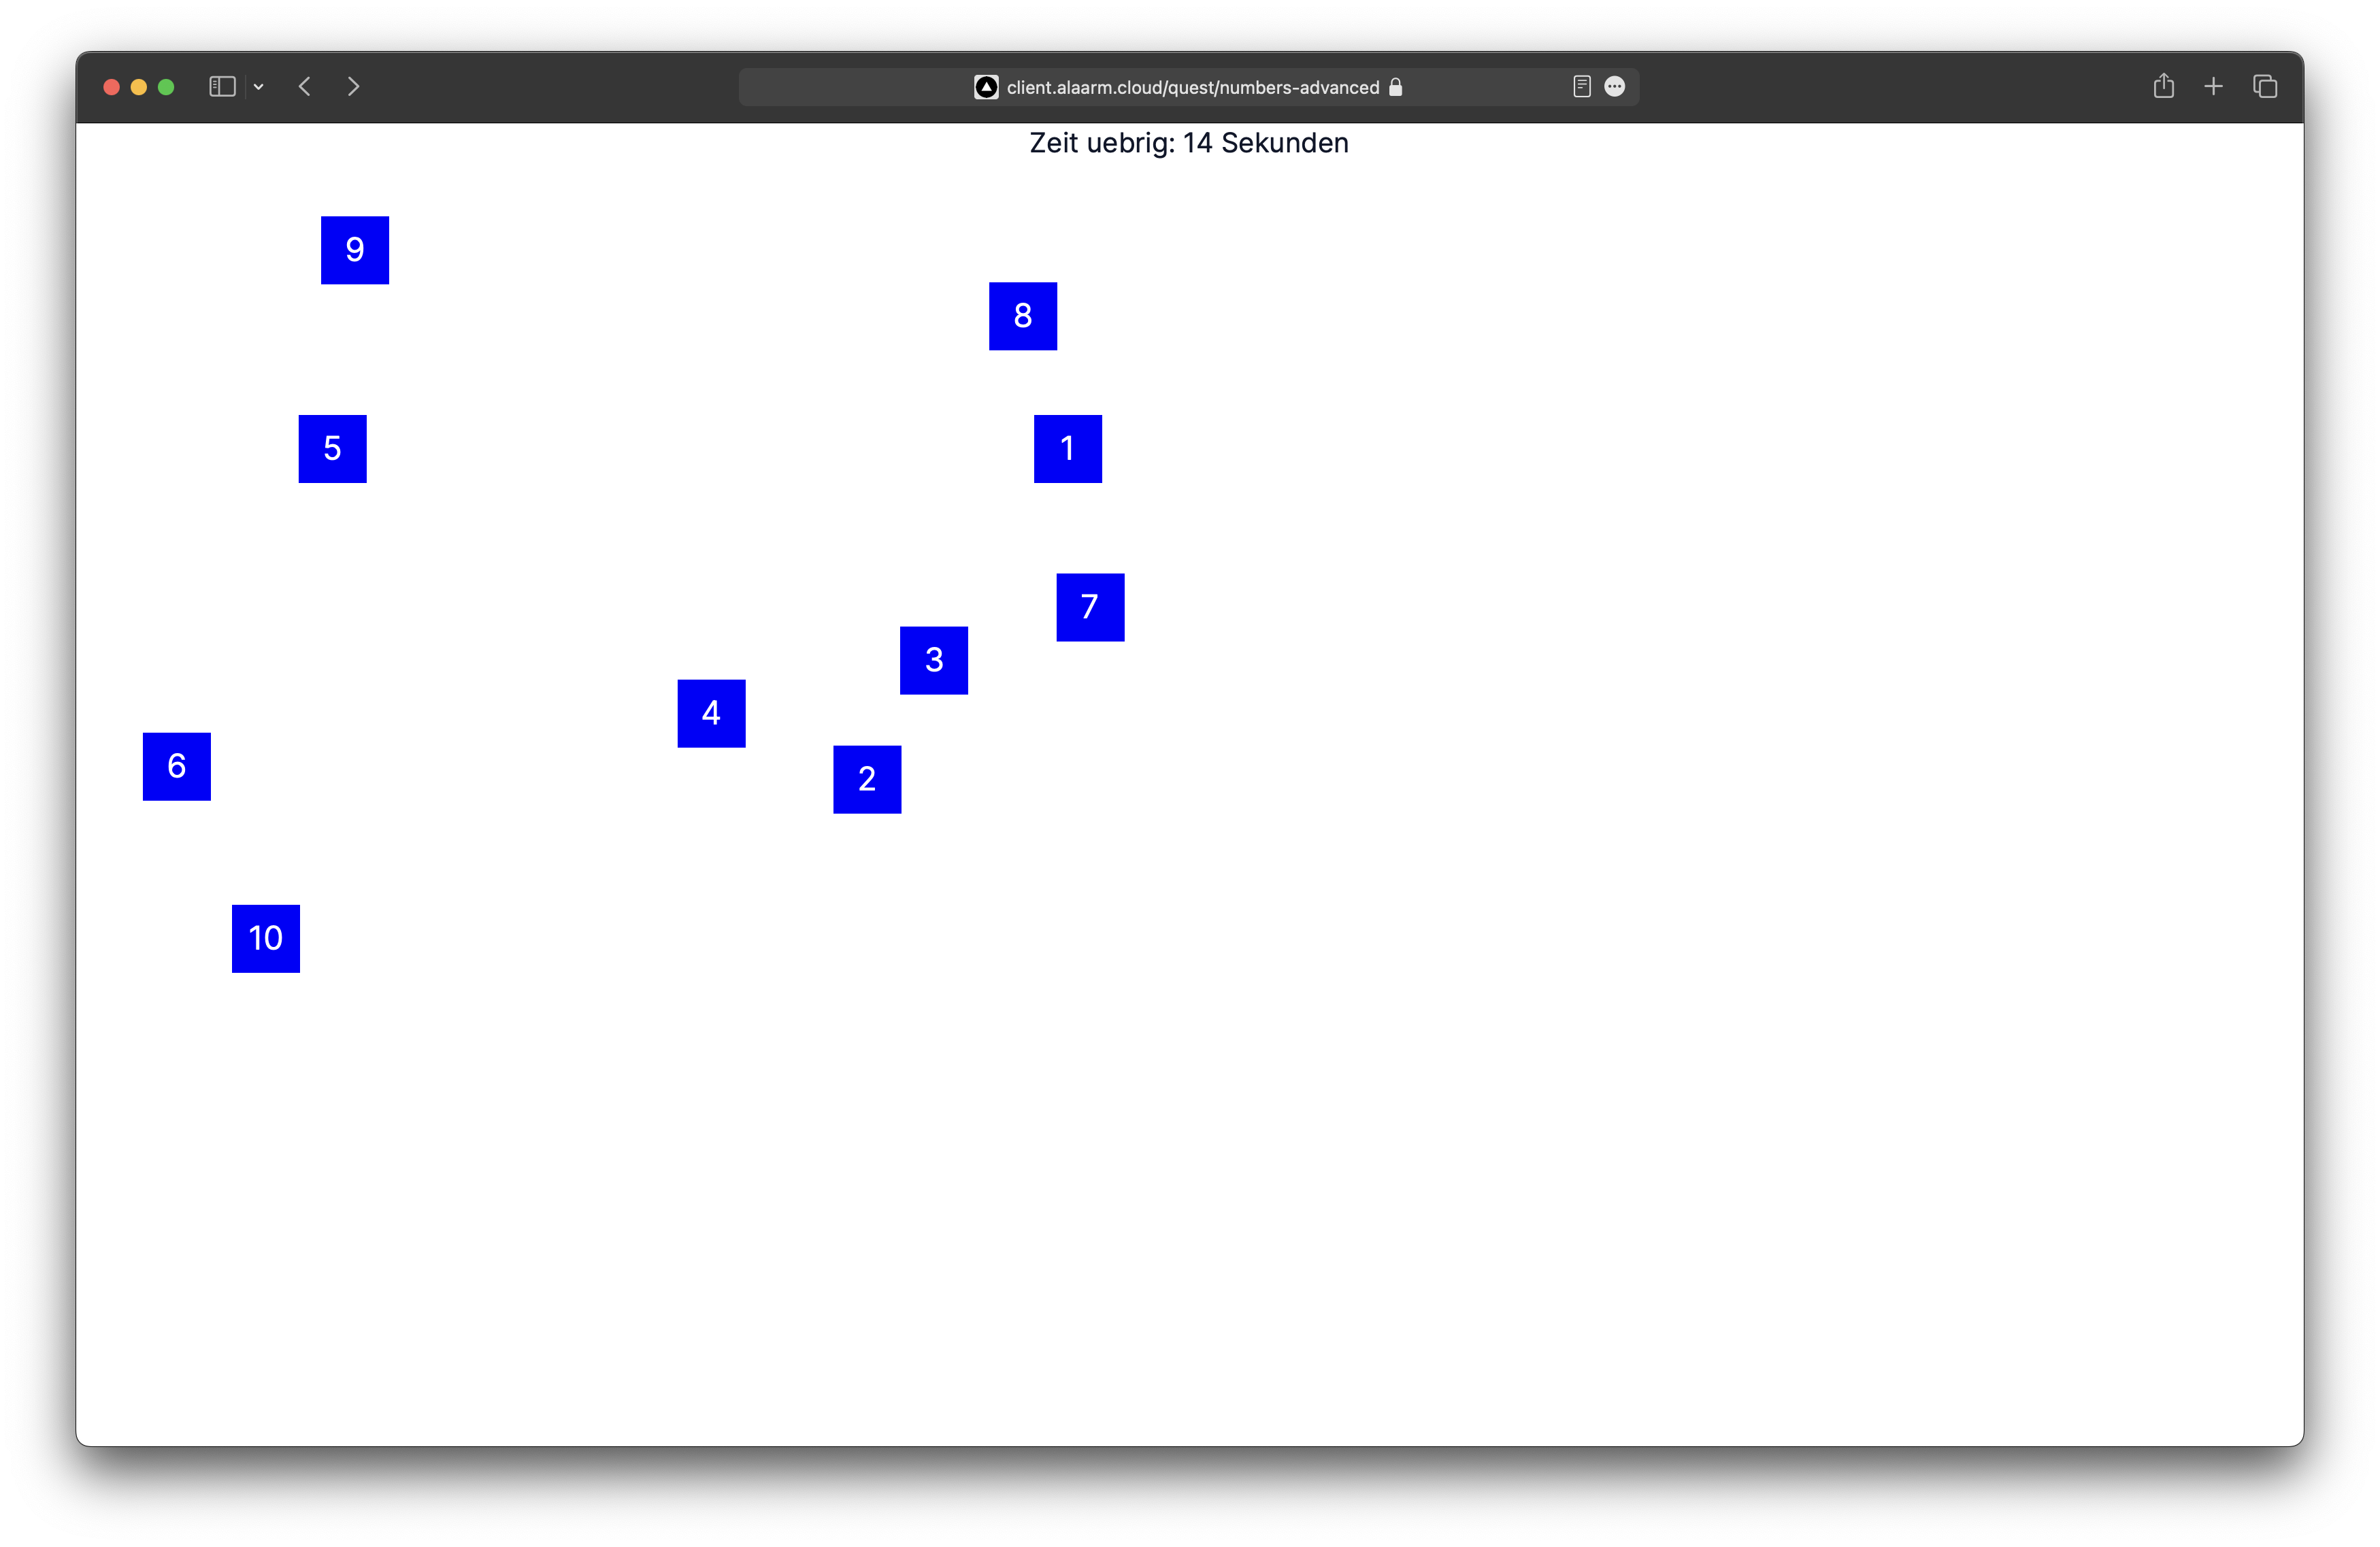
\includegraphics[width=15cm, height=9.61cm]{res/quest_02.png}
   \caption{Rätsel 2}
\end{figure}

In dem potentiell letzten, \textbf{dritten Störungsvorgang} des MVPs \textit{Problem K1213 mit der Kalibrierung} ist ein schwerwiegendes Fehlerbild in der Kalibrierung der Maschine zu beheben. Durch eine Fehlkalibrierung ist es zu einem Kabelbrand gekommen. Um den Schaden zu begrenzen, müssen die Eingaben schnellstmöglich neu kalibriert werden, um einen Brand zu verhindern. Zur korrekten Kalibrierung muss ein grün aufleuchtender Bereich auf der Weboberfläche des Übungsteilnehmers innerhalb von 0,6 Sekunden gedrückt werden. Der Bereich ist dabei initial schwarz gefärbt. Im Falle einer rechtzeitigen Reaktion ist die Maschine kalibriert, eine Ausweitung des Brandes abgewandt und das Szenario erfolgreich beendet. Das Kalibrierungsrätsel ist folgender Abbildung zu entnehmen:

\begin{figure}[H]
   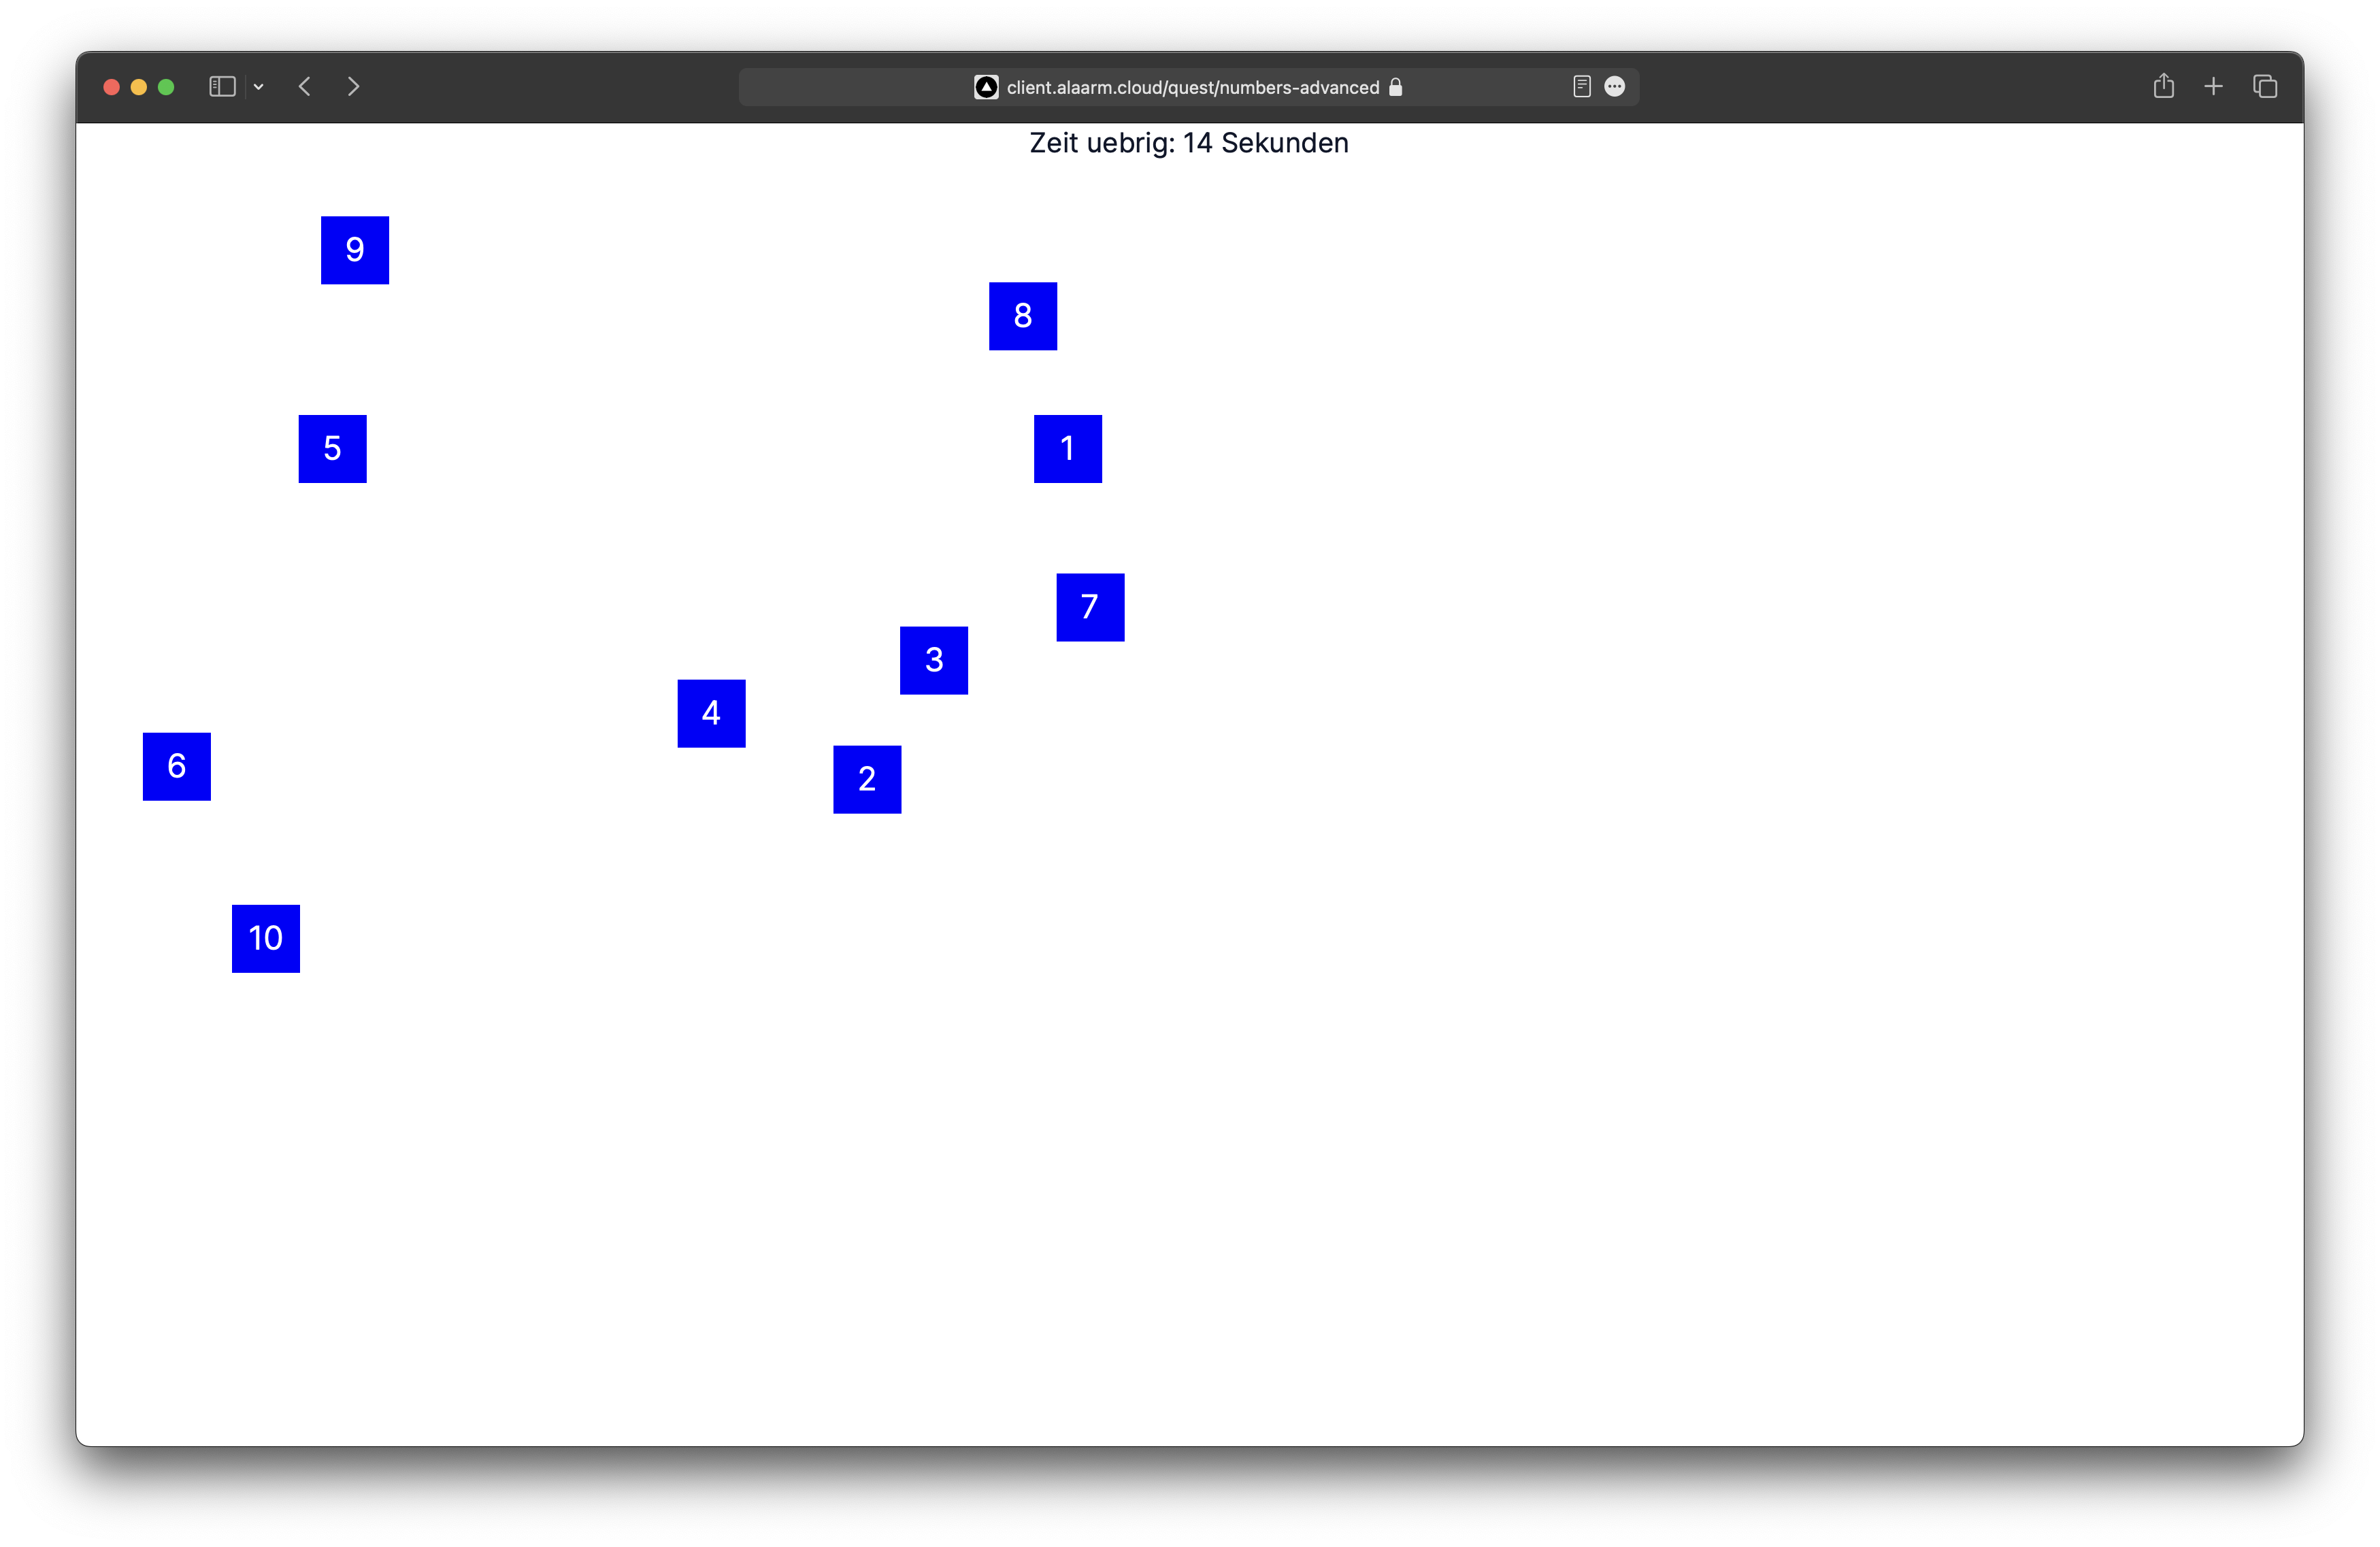
\includegraphics[width=15cm, height=9.61cm]{res/quest_02.png}
   \caption{Rätsel 3}
\end{figure}

\subsubsection{Administration der Alarmsimulation}

Die Verantwortung und Steuerung der Alarmsimulation wird durch den Übungsleiter getragen. Neben dem Start der Simulation kann auf einer Web-Oberfläche des Admintablets das Szenario individuell konfiguriert werden. Beispielsweise können Anpassungen wie veränderte Sounddateien, weitere Eskalationsstufen, Zufallsvariablen für die Erfolgswahrscheinlichkeit einer Entstörung und Zeiträume zur Lösung einer Eskalationsstufe definiert werden.

\subsection{Begleitende Dokumente}
\usepackage{hyperref} 
Für die Simulation wurde eine generelle Bedienungsanleitung und ein Sicherheitsbriefingbogen entworfen, um den Übungsleiter bei der Anleitung von neuen Übungsteilnehmern zu unterstützen. Jene Dokumente können dem \hyperref[sec:anhang]{Anhang} entnommen werden.

\begin{comment}
\subsection{Sicherheitsbriefing}\hspace{0pt}\marginpar{\footnotesize{ca. 2 Min.}}

\emph{Bitte nehmen Sie sich die Zeit, diese Anweisungen sorgfältig zu lesen und zu verstehen, bevor Sie mit dem Betrieb der Maschine fortfahren. Ihre Sicherheit hat oberste Priorität.}

\newpage

\emph{WICHTIG: GESUNDHEITSWARNUNG \\
Bitte stellen Sie sicher, dass Sie die geeignete Schutzkleidung tragen, bevor Sie mit dem Betrieb dieser Maschine beginnen. Dies beinhaltet Schutzhandschuhe, Schutzbrille und Atemschutzmaske. Bitte entnehmen Sie die Schutzkleidung, die rechts von Ihnen liegt. 
Es besteht die Möglichkeit, dass während des Szenarios Rauch oder andere intensiv riechende Substanzen verwendet werden.
Dieses Szenario beinhaltet flackernde Lichter, die bei einigen Personen mit Epilepsie zu Anfällen führen können. 
Bitte beachten Sie, dass Ihre Gesundheit und Sicherheit oberste Priorität haben. Falls Sie Bedenken haben oder gesundheitliche Einschränkungen haben, die sich auf Ihre Teilnahme an diesem Szenario auswirken könnten, empfehlen wir Ihnen, vorab Rücksprache mit einem Arzt zu halten, um sicherzustellen, dass Sie angemessen geschützt sind und das Szenario ohne Risiken für Ihre Gesundheit durchführen können.}

\

\subsection{Bedienungsanleitung und Aktivierung der Eskalationsstufe}
\

\emph{BEDIENUNGSANLEITUNG \\
1.	Überprüfen Sie, ob alle Sicherheitsvorkehrungen getroffen wurden und die Maschine bereit für den Betrieb ist. \\
2.	Drücken Sie den grünen Startknopf auf der rechten Seite des Bedienfelds, um den Maschinenprozess zu starten. \\
3.	Überwachen Sie den Prozess auf dem Bildschirm. Achten Sie auf alle Warnungen oder Fehlermeldungen, die angezeigt werden könnten. \\
4.	Im Falle einer Fehlermeldung, drücken Sie den roten Stopp-Knopf und befolgen Sie die Anweisungen auf dem Bildschirm. \\
5.	Wenn der Prozess abgeschlossen ist, drücken Sie den blauen Reset-Knopf, um die Maschine auf ihren Ausgangszustand zurückzusetzen.}

\

\textbf{\underline{Start:}}
\end{comment}

\subsection{Prozessmodell}
\label{chap:process model} 
\begin{figure}
    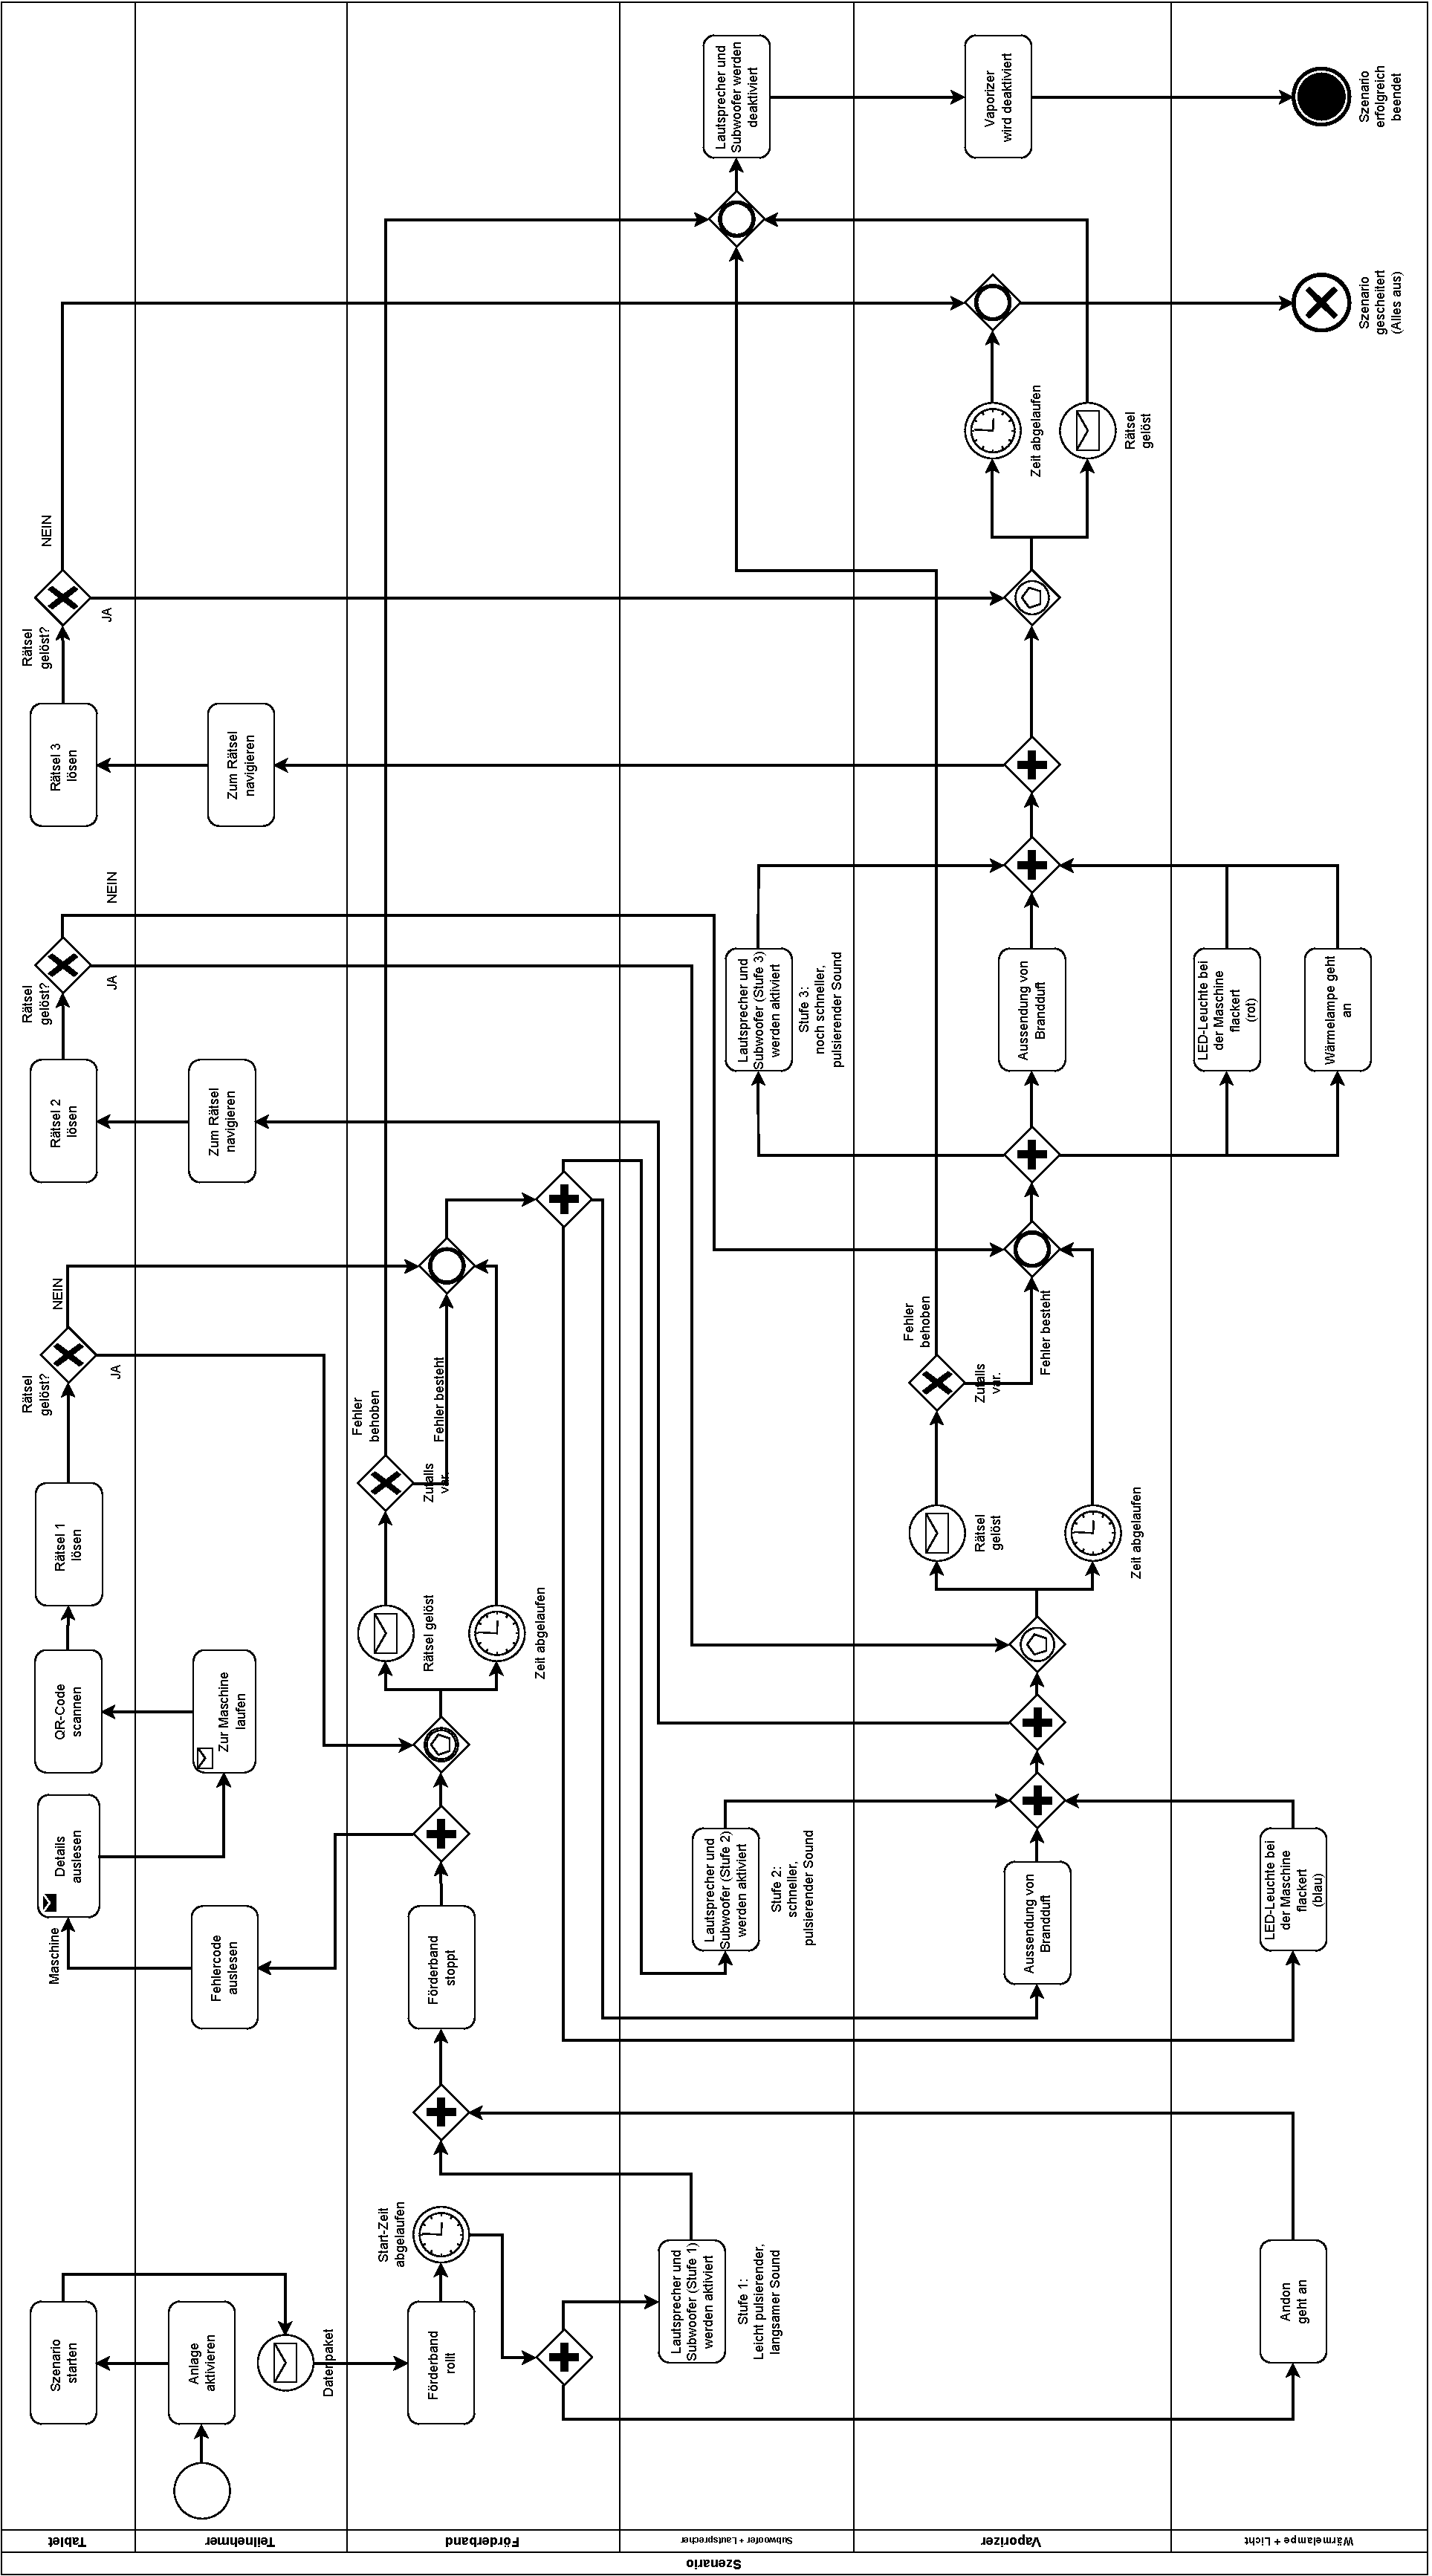
\includegraphics[scale=0.37]{res/Finales Szenario BPMN(korrigiert).drawio-5.pdf}
    \caption{BPMN-Diagramm}
\end{figure}

Die nachfolgende Abbildung veranschaulicht den detaillierten Ablauf des Szenarios in Form eines BPMN-Diagramms mit insgesamt sechs Swimlanes. Dabei repräsentieren die Swimlanes die Komponenten ''Tablet'', ''Teilnehmer'' und ''Förderband''.

Die Komponenten, die im Verlauf des Szenarios zur Immersion genutzt werden, sind entsprechend ihrer Wahrnehmungsart in drei unterschiedliche Swimlanes aufgeteilt. Die Swimlane \textit{Subwoofer+Lautsprecher} widmet sich den auditiven Komponenten, während die Swimlane \textit{Vaporizer} die Geruchs-Aspekte des Szenarios skizzieren. Zusätzlich bezieht sich die Swimlane \textit{Wärmelampe+Licht} auf die Prozesselemente mit visuellen Komponenten.


\begin{comment}
\section{Prozessmodellierung}

%Sätze beginnen alle mit Die...Die...Die. Evtl. abändern wenn euch eine bessere Formulierung einfällt.
Die folgende Abbildung stellt den detaillierten Prozessablauf des Szenarios in Form eines BPMN-Diagramms dar. \\
Das Diagramm besteht aus sechs Swimlanes. Die Komponenten „Tablet“, „Teilnehmer“ und „Förderband“ werden durch je eine Swimlane abgebildet. Die im Laufe des Szenarios zur Immersion eingesetzten Komponenten sind nach der Art ihrer Wahrnehmung in drei verschiedene Swimlanes unterteilt. Die Swimlane „Subwoofer+Lautsprecher“ bezieht sich auf den die auditiven Komponenten. Die Swimlane „Vaporizer“ beschreibt die Elemente des Szenarios mit Bezug auf olfaktorische Wahrnehmung. Die Swimlane „Wärmelampe+Licht“ bezieht sich auf die Prozesselemente mit visuellen Komponenten.


\begin{figure}
    \caption{BPMN-Diagramm}
    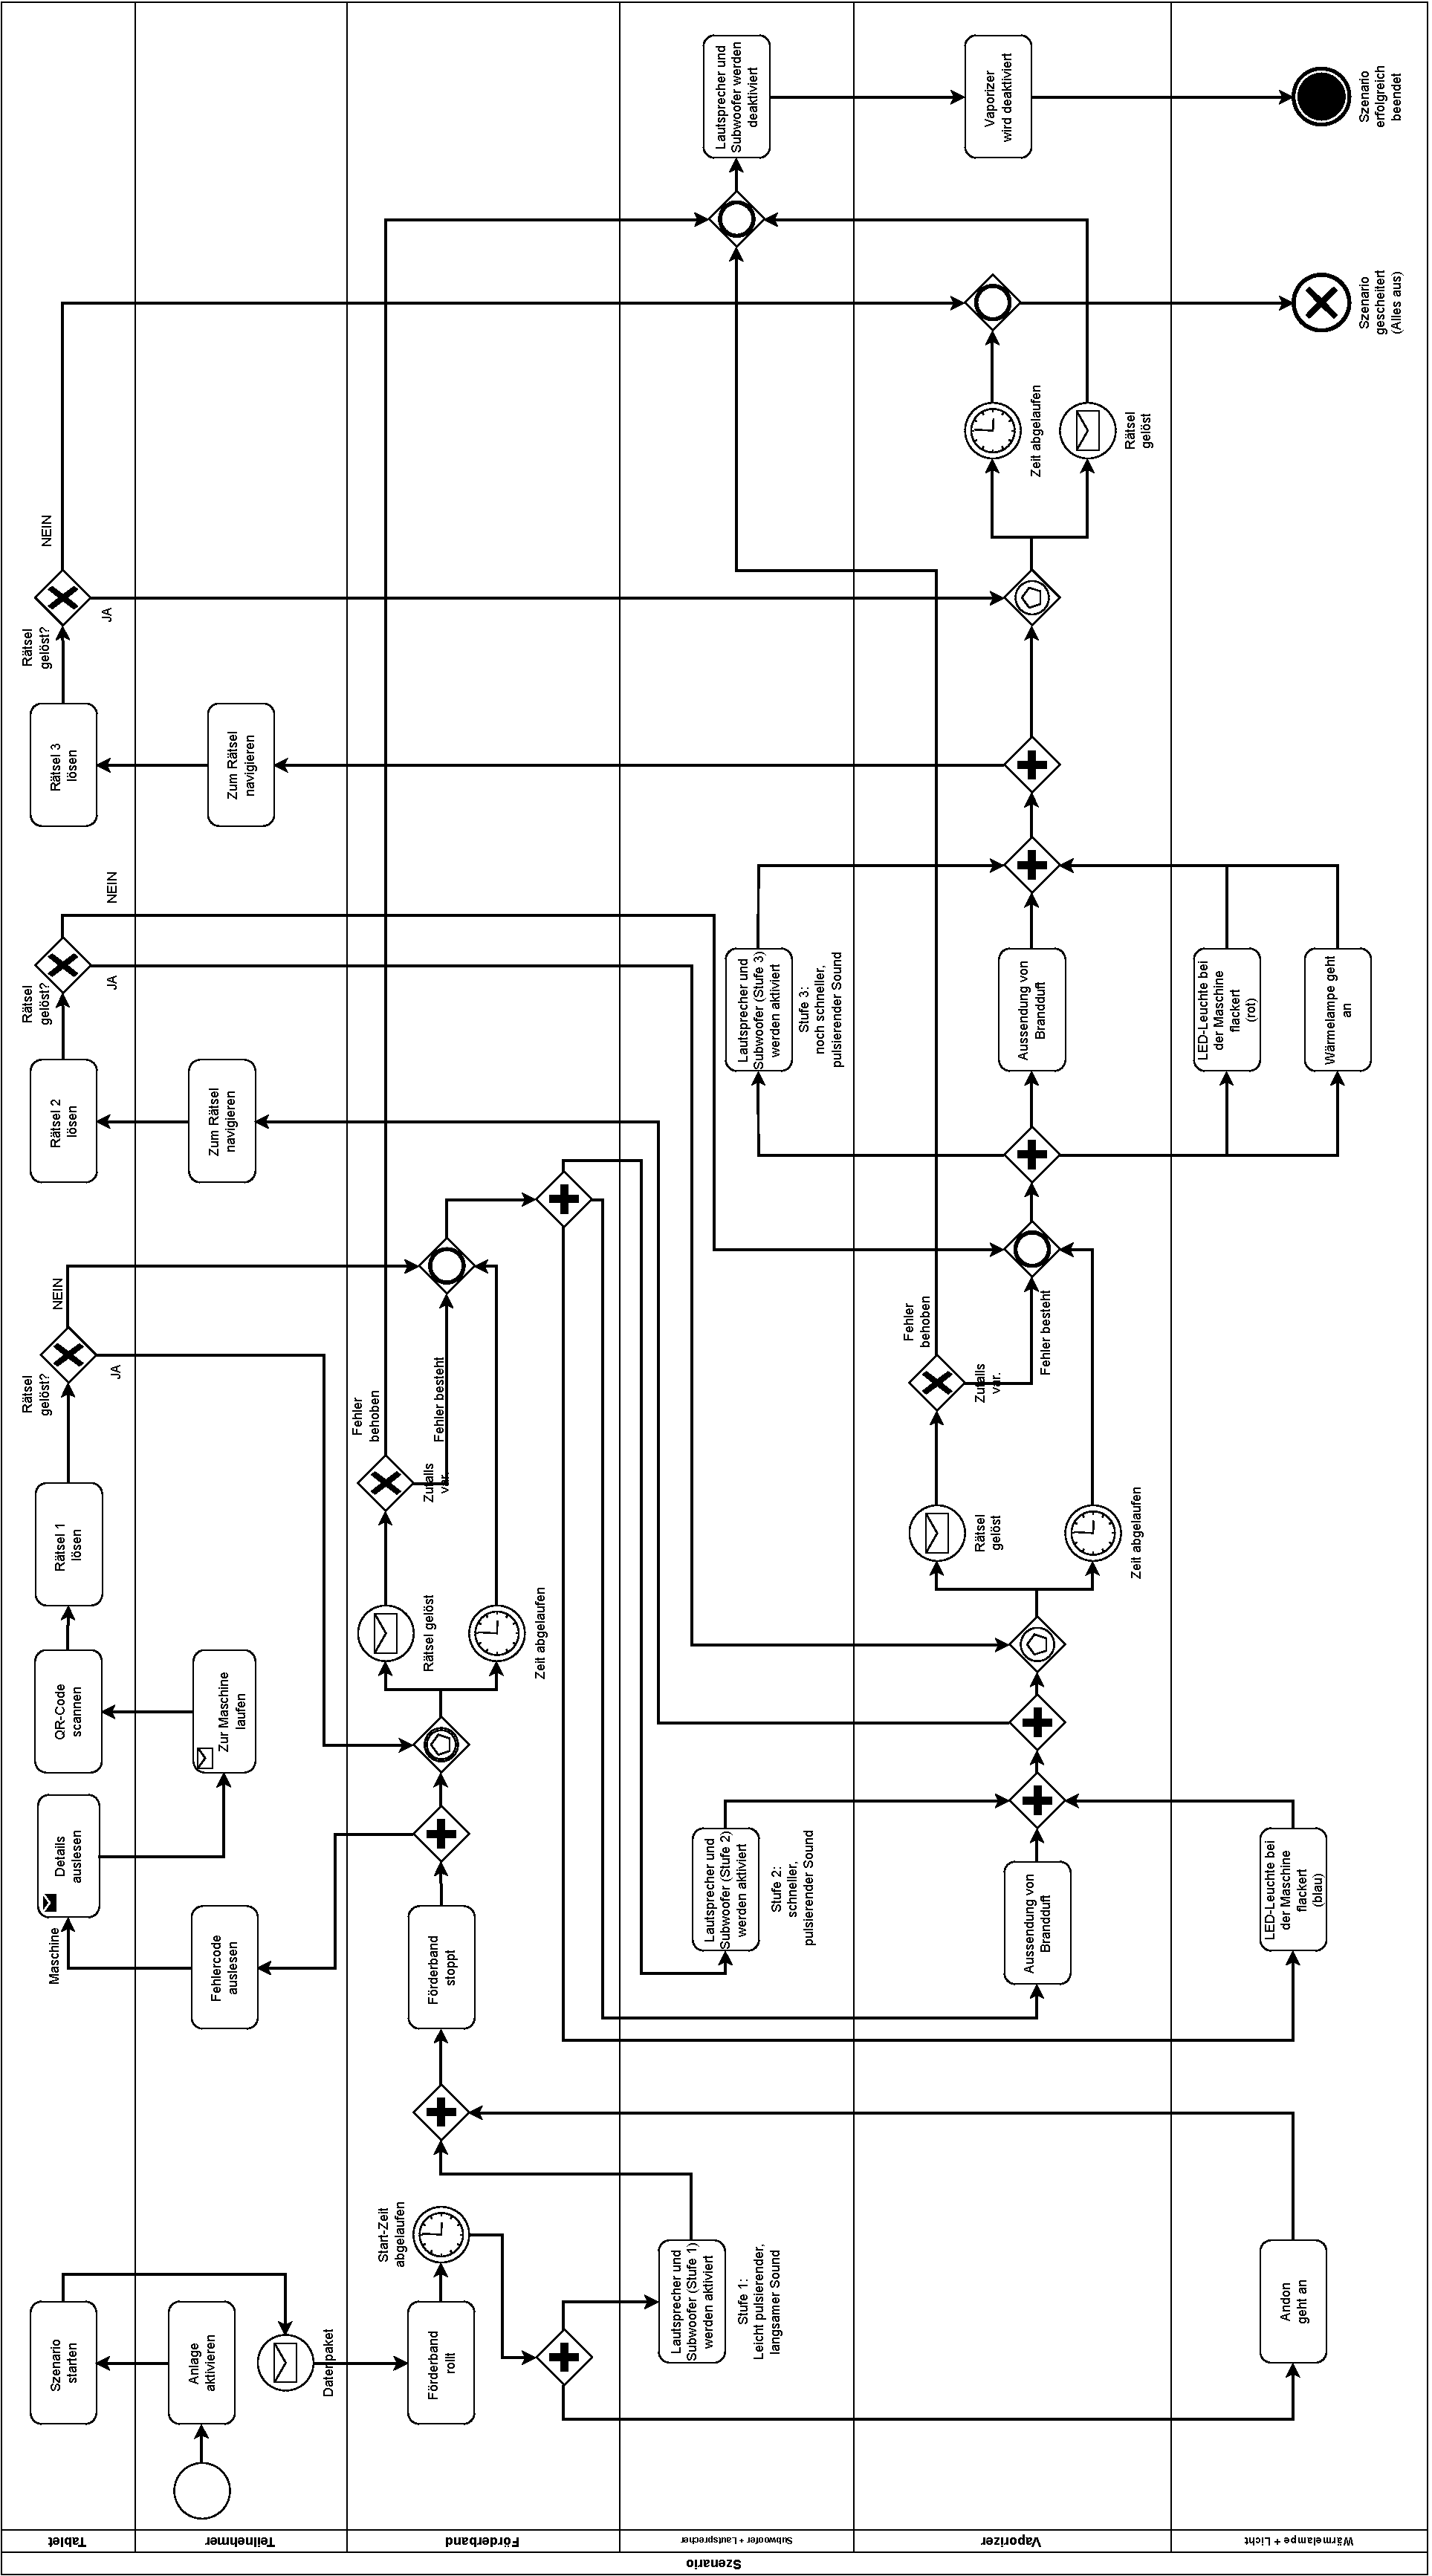
\includegraphics[scale=0.37]{res/Finales Szenario BPMN(korrigiert).drawio-5.pdf}
\end{figure}
\end{comment} \clearpage
\section{Technische Umsetzung des Protoypen}

Im folgenden Abschnitt wird auf die Implementierung des Alarmszenarios und dazugehörige Überlegungen eingegangen. Zu Beginn wird der gewählte Technologie-Stack dargelegt und durch Ausführungen zur Systemarchitektur ergänzt. 
Daran schließt ein Abschnitt zur Erklärung der Konfigurationen von Alarmszenarien als auch der eingesetzten APIs an.

\subsection{Technologie-Stack}

Die Auswahl des Technologie-Stacks zur Implementierung von ALAARM-ZIP hängt zentral von einer Vielzahl von Vorbedingungen ab.


Bezüglich der verwendeten \textbf{Programmiersprache} wurde sich für den Einsatz von \textit{TypeScript}\footnote{Siehe \href{https://typescriptlang.org/}{https://typescriptlang.org/}} entschieden. Neben der Eignung für Webapplikation und der universellen Verwendbarkeit, d.h. der Möglichkeit, die Anwendung sowohl via Browser (Windows, iPadOS, Linux) als auch serverseitig auszuführen,  waren sprachenspezifische Eigenschaften wie Typisierung für die Projektgruppe entscheidend, um sich auf \textit{TypeScript} festzulegen.

Für das \textbf{Frontend} wurde sich für \textit{NextJS}\footnote{Siehe \href{https://nextjs.org/}{https://nextjs.org/}} als spezifisches \textit{React}-Framework entschieden. Hiermit können Elemente einer Website bereits serverseitig gerendert werden, bevor sie zum Client gesendet werden, ebenso wird ein Routing mitgeliefert. Zusätzlich erfolgt der Einsatz der UI-Komponentenbibliothek \textit{ShadCN}\footnote{Siehe \href{https://ui.shadcn.com/}{https://ui.shadcn.com/}}, welche auf dem CSS-Framework \textit{TailwindCSS}\footnote{Siehe \href{https://tailwindcss.com/}{https://tailwindcss.com/}} basiert. 

Für den \textbf{Controller} wurde sich für die \textit{NodeJS}\footnote{Siehe \href{https://nodejs.org/}{https://nodejs.org/}} Laufzeitumgebung aufgrund der ereignisgesteuerten I/O-Architektur für Echtzeitanwendungen entschieden. \textit{REST APIs} werden beim Controller dafür genutzt, um einen Kommunikationsfluss zwischen Admin-Panel, Client und MQTT-Server zu realisieren (Systemarchitektur siehe Kapitel \ref{chap:systemarchitecture}). Durch die Verbindung mit \textit{MQTT} können Nachrichten unmittelbar an den MQTT-Broker gesendet werden.

Für die \textbf{Entwicklung} wurde ein \textit{git-Repository}\footnote{Siehe \href{https://git-scm.com/}{https://git-scm.com/}} aufgesetzt, welches durch den Anbieter Github\footnote{Siehe \href{https://github.com/}{https://github.com/}} bereitgestellt wird. Das Repository inkl. vollständiger technischer Dokumentation kann unter folgendem Link eingesehen werden:  \url{https://github.com/ToKoSoftware/up-alaarm-zip}. Die Verwaltung des Mono-Repositories erfolgte mit \textit{Lerna}\footnote{Siehe \href{https://lerna.js.org/}{https://lerna.js.org/}}. Zur Paketverwaltung wurde auf \textit{npm}\footnote{Siehe \href{https://npmjs.com/}{https://npmjs.com/}}  zurückgegriffen. Um einen einheitlichen Codestyle zu erzwingen, wurden die Pakete \textit{Prettier}\footnote{Siehe \href{https://prettier.io/}{https://prettier.io/}} und \textit{ESLint}\footnote{Siehe \href{https://eslint.org/}{https://eslint.org/}} genutzt. Mithilfe von \textit{Husky}\footnote{Siehe \href{https://typicode.github.io/husky/}{https://typicode.github.io/husky/}} wurden diese Tools vor jedem Commit automatisiert ausgeführt. Das Deployment auf einem Web-Server des Anbieters \textit{Vercel}\footnote{Siehe \href{https://vercel.com/}{https://vercel.com/}} erfolgt automatisiert on-push auf den \textit{main branch} des git-Repository.


\subsection{Systemarchitektur}
\label{chap:systemarchitecture}
Der folgenden Abbildung ist die Systemarchitektur von ALAARM-ZIP zu entnehmen:

\begin{figure}[h]
   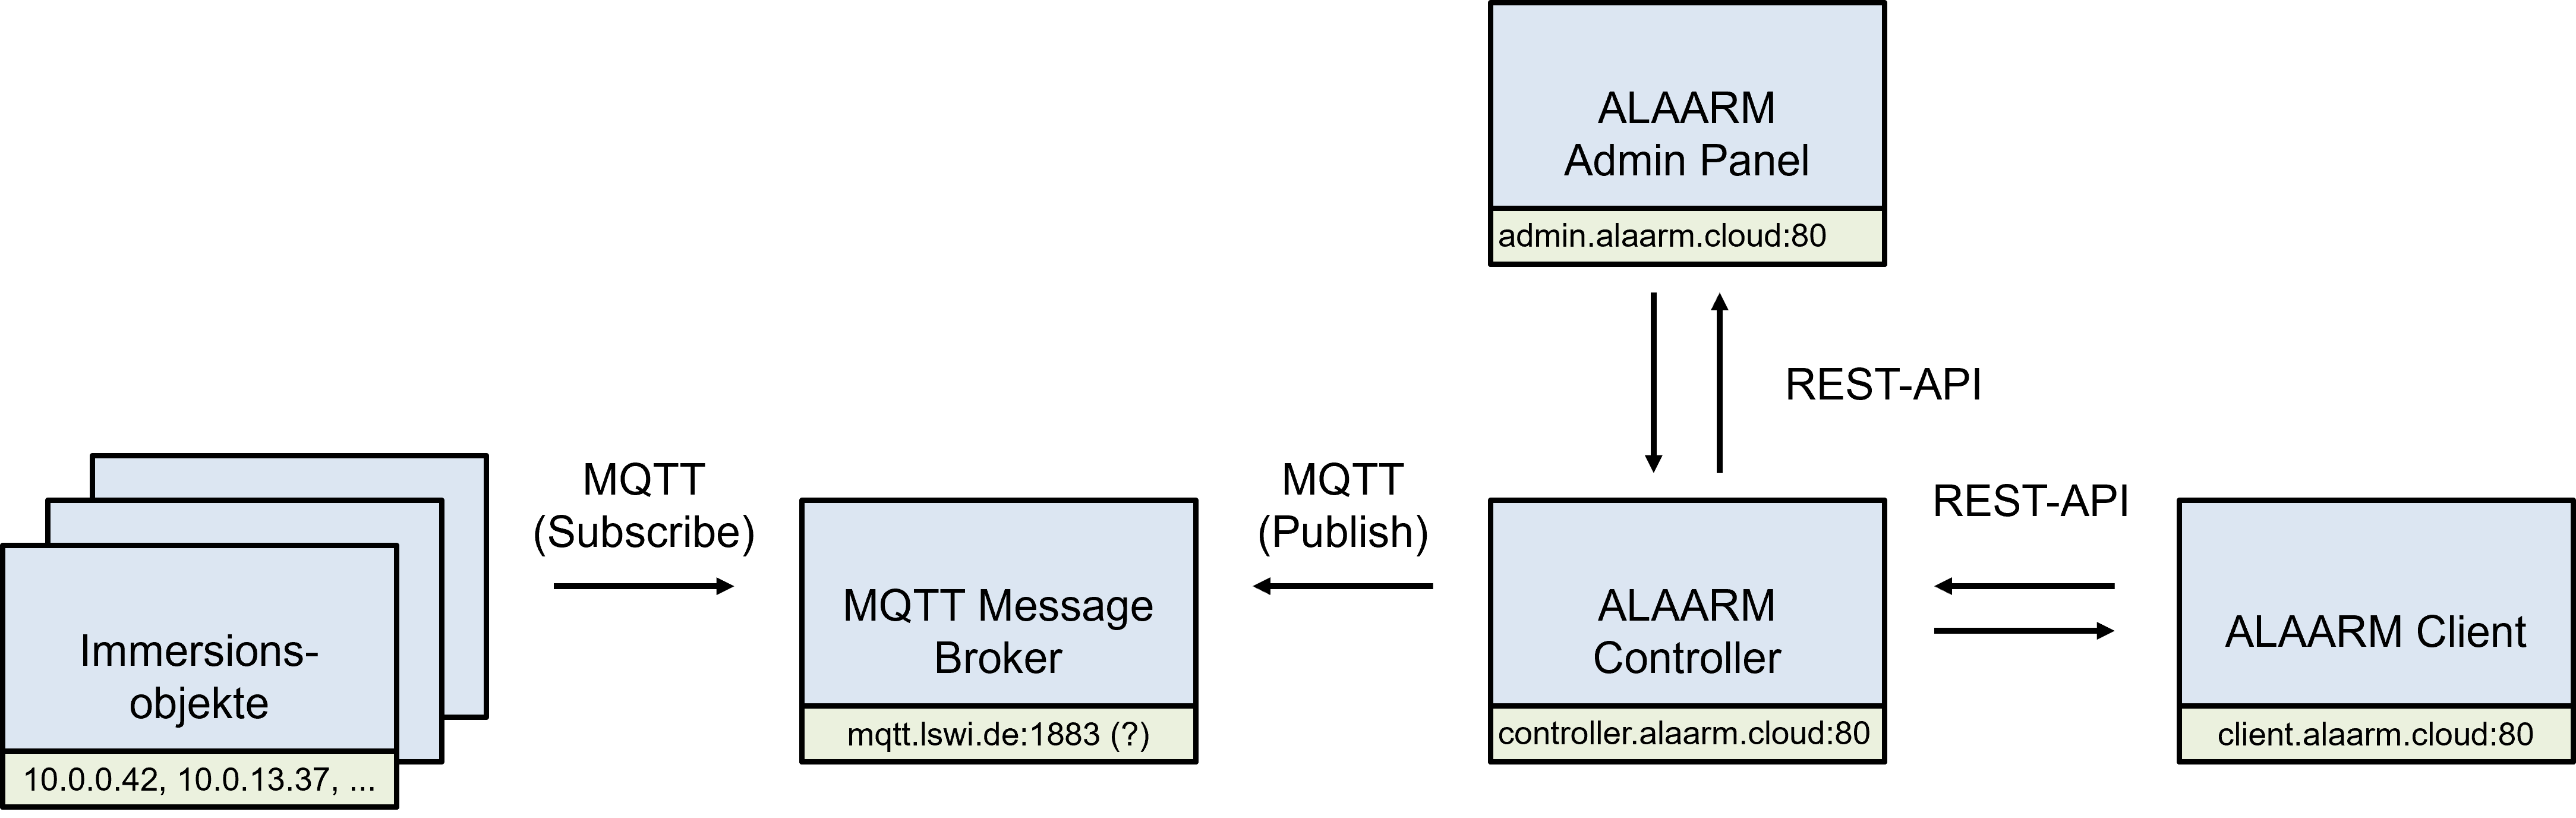
\includegraphics[width=15cm, height=5.87cm]{res/20230809_architecture.png}
   \caption{Systemarchitektur}
\end{figure}


Den Kernkommunikationshub nimmt der \textit{ALAARM Controller} ein, welcher die Kommunikation zwischen dem Admin Panel, dem Client und dem MQTT Message Broker übernimmt. Das Admin Panel ist die Steuerung des Administrators, welcher verantwortlich für die Entwicklung und das Management von Szenarien für die Simulation ist.
Das \textit{Admin Panel} ist auf \href{https://admin.alaarm.cloud/}{https://admin.alaarm.cloud/} bereitgestellt.
Die \textit{ALAARM Client} Komponente verarbeitet die Eingaben auf dem Tablet von Simulationsteilnehmern und bildet die Rätsellogik ab. Ebenso realisiert diese Komponente die QR-Scanner Funktionalität, damit via QR Codes Rätsel durch Simulationsteilnehmer aufgerufen werden können. Bereitgestellt wird der Client auf \href{https://client.alaarm.cloud/}{https://client.alaarm.cloud/}.

Mithilfe des \textit{MQTT Message Brokers} können über den Controller Events übergeben werden, welche durch MQTT an die entsprechend adressierten und angebundenen Immersionsobjekte wie den Subwoofer übergeben werden. Entsprechende Datenobjekte werden durch die \textit{Immersionsobjekte} schlussendlich ausgeführt. Bei Ansteuerung kann ein Subwoofer beispielsweise einen kräftigen Druckstoß durchführen, nachdem ein Rätsel nicht im definierten Zeitrahmen gelöst worden ist und das Szenario eine neue Eskalationsstufe aufruft. 

\subsection{Konfiguration von Alarmszenarien}

Zu Beginn einer geplanten Alarmsimulation kann durch den Administrator das zu durchlaufende Szenario konfiguriert werden. Hierfür ist zunächst die Adresse \href{https://admin.alaarm.cloud}{https://admin.alaarm.cloud} aufzurufen. Mit dem Klick auf den schwarzen Button \textit{\enquote{Szenario starten}} öffnet sich auf der rechten Seite die Seitenleiste zur Konfiguration des Szenarios. Zunächst ist durch den Admin mithilfe eines Unique Resource Identifiers die Adresse des Controllers anzugeben, damit die gewünschte Ablaufsteuerung für die Simulation geladen werden kann. Zur Authentifizierung des Administrators ist als Nächstes das festgelegte Secret einzugeben. Daran schließt das Eingabefeld an, in welches Daten zur Spezifizierung des Szenarios im JSON-Formformat übermittelt werden müssen.
Schlussendlich kann die Simulation des Szenarios über einen Klick des schwarzen Buttons \textit{\enquote{Szenario starten}} in der Seitenleiste begonnen werden.

Dabei empfängt der adressierte Controller die angegebene Konfiguration und beginnt entsprechend der Ablauflogik Messages an die Immersionsgeräte zu verteilen.

\begin{figure}[h]
   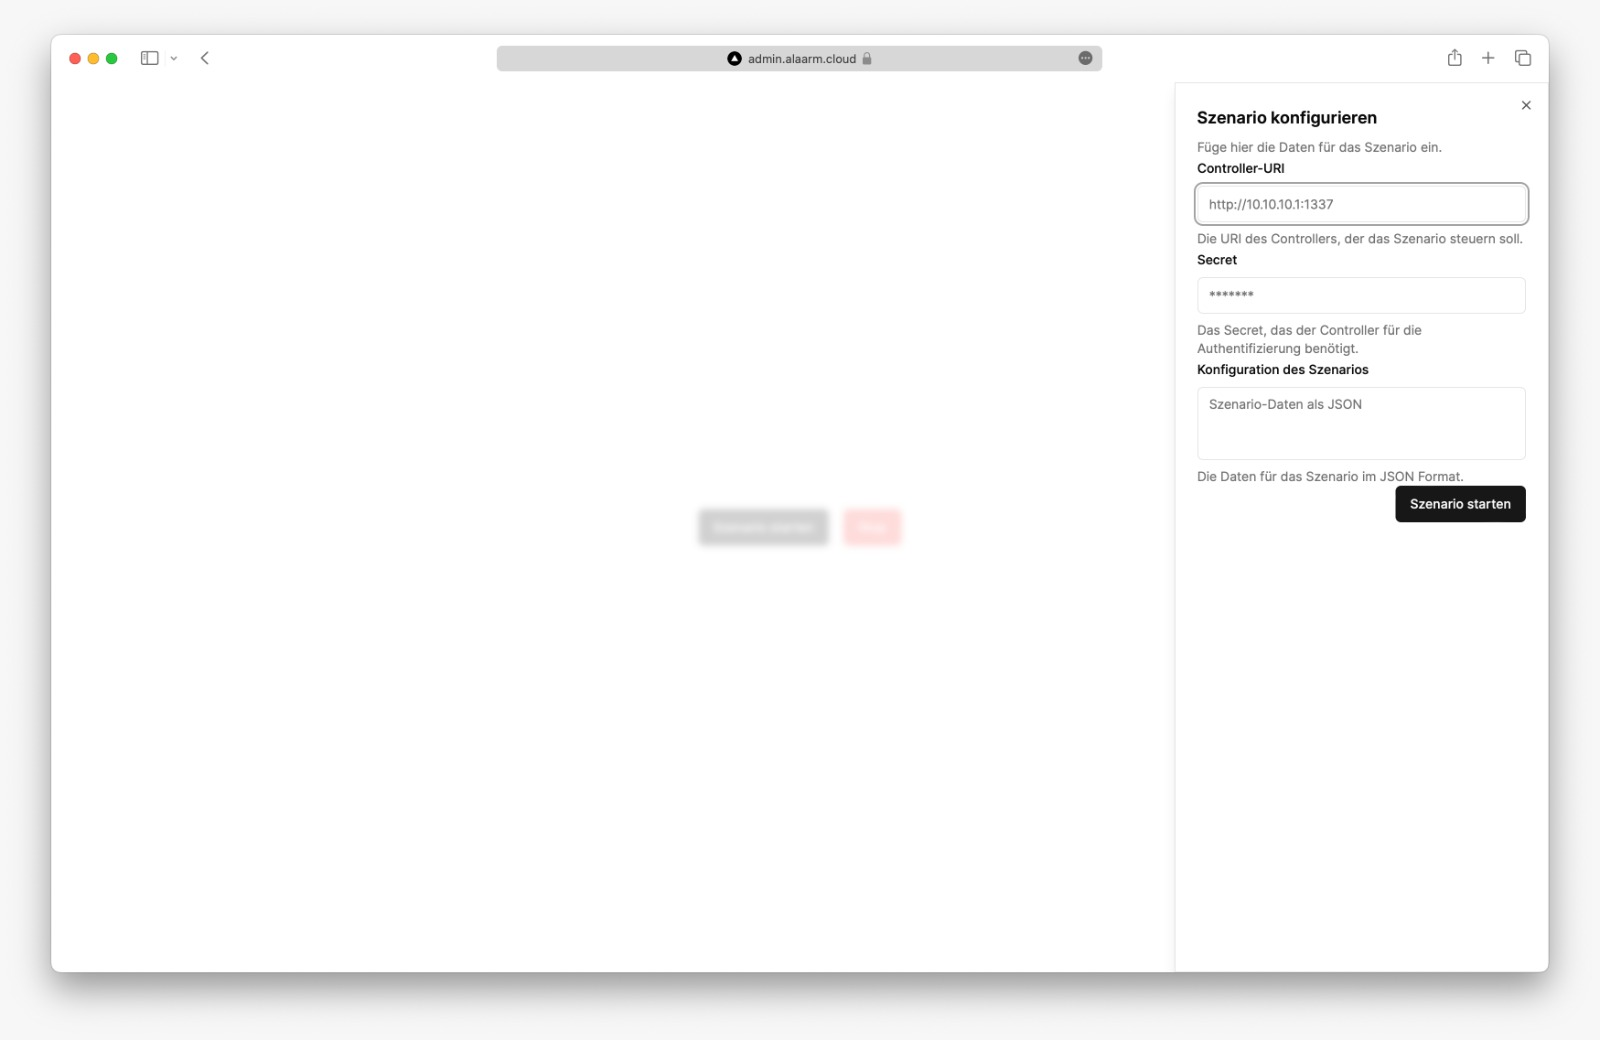
\includegraphics[width=15cm, height=10.87cm]{res/20230821_Szenario_Configuration.jpg}
   \caption{Szenariokonfiguration}
\end{figure}



\newpage
\subsection{APIs}

Zur Kommunikation verschiedener Komponenten untereinander kommen RESTful APIs und das MQTT Message Protocol zum Einsatz. 

Requests via RESTful API verfügen über ein Datenobjekt, welches je nach Anfrage etwa dem Start eines Szenarios (\textit{api/v1/scenario/start}) variabel ausfällt. Der Start und Stopp von Szenarien wird über POST Requests zum Anlegen jener neuen Ressource abgewickelt. Zum Abrufen von Daten wie Rätseln oder dem Status, etwa ob ein Rätsel rechtzeitig gelöst worden ist, werden GET Requests genutzt \autocite{masse2011rest}.

Um Immersionsobjekte zur Auslösung von Immersionseffekten wie Licht und Geräusche anzusteuern, wird das MQTT Message Protocol verwendet. Die Ansteuerung erfolgt über festgelegte \textit{Event Types}. Bei der Ansteuerung wird ein \textit{Payload}, etwa ein Link zu einer .mp3 Datei, übergeben, um von Seite des Immersionsobjekts den gewünschten Effekt auszuführen.
 \clearpage
\section{Fazit}

Die vorliegende Projektdokumentation beschrieb die Schaffung einer Simulation von Alarmszenarien im Kontext des Themenfelds Industrie 4.0. 

Die Projektarbeit konzentrierte sich darauf, Alarmszenarien im Industrie-4.0-Kontext zu entwickeln und durch spezifische Komponenten die Immersion dieser Szenarien zu intensivieren. Die Integration eines Minimum Viable Products (MVP) in die Simulationsumgebung des Zentrums Industrie 4.0 ermöglicht es, Störfallszenarien realitätsnah zu simulieren und die Reaktionen der Teilnehmer zu beobachten. Dies eröffnet neue Möglichkeiten für die Mensch-Maschine-Interaktion und die Bewertung von Verhaltensweisen in Gefahrensituationen im Kontext zunehmend vernetzter Produktionsumgebungen.

Die entworfenen Alarmszenarien eröffnen nicht nur neue Forschungspotenziale, sondern können auch zur Entwicklung von Schulungsprogrammen und Übungen genutzt werden, um das Bewusstsein und die Fähigkeiten der Mitarbeiter im Umgang mit potenziellen Gefahren zu stärken. Zudem besteht anhand dieser Projektdokumentation und dem gegebenen \textit{git-Repository} die Möglichkeit, die Alarmsimulation durch neu zu definierende Szenarien und einzuführende Komponenten mit geringem Aufwand zu erweitern.
 \clearpage
\section*{Anhang}
\label{sec:anhang}

\subsection*{Sicherheitsbriefing}\hspace{0pt}\marginpar{\footnotesize{ca. 2 Min.}}
\emph{Bitte nehmen Sie sich die Zeit, diese Anweisungen sorgfältig zu lesen und zu verstehen, bevor Sie mit dem Betrieb der Maschine fortfahren. Ihre Sicherheit hat oberste Priorität.}

\emph{WICHTIG: GESUNDHEITSWARNUNG} \\

\emph{Bitte stellen Sie sicher, dass Sie die geeignete Schutzkleidung tragen, bevor Sie mit dem Betrieb dieser Maschine beginnen. Dies beinhaltet Schutzhandschuhe, Schutzbrille und nach Anweisung des Übungsleiters eine Atemschutzmaske. 
Es besteht die Möglichkeit, dass während des Szenarios Rauch oder andere intensiv riechende Substanzen verwendet werden.
Dieses Szenario beinhaltet flackernde Lichter, die bei einigen Personen mit Epilepsie zu Anfällen führen können. Bitte beachten Sie, dass Ihre Gesundheit und Sicherheit oberste Priorität haben. Falls Sie Bedenken haben oder gesundheitliche Einschränkungen haben, die sich auf Ihre Teilnahme an diesem Szenario auswirken könnten, empfehlen wir Ihnen, vorab Rücksprache mit einem Arzt zu halten, um sicherzustellen, dass Sie angemessen geschützt sind und das Szenario ohne Risiken für Ihre Gesundheit durchführen können.}

\subsection*{Beschreibungskarte MVP}

In diesem Szenario wird ein Ablauf aus verschiedenen Komponenten und Eskalationsstufen beschrieben, das in der Simulationsumgebung des Zentrums Industrie 4.0 implementiert wurde. Die Szenariokomponenten bestehen aus den Teilnehmern, Tablet, Subwoofer/Lautsprecher, Wärmelampe/Licht und Nebelmaschine. Diese Komponenten sind in einer Umgebung platziert, in der es Anlagen zum Bedienen gibt, die alle durch ein Förderband miteinander verbunden sind. Das System ist so konzipiert, dass es drei Eskalationsstufen gibt, die nacheinander aktiviert werden können. Jede Eskalationsstufe beinhaltet einen Entstörungsvorgang, der vom Teilnehmer gelöst werden muss. Dabei werden verschiedene Szenariokomponenten aktiviert, um den Prozess zu unterstützen und zu simulieren. Teilnehmer des Szenarios, die bei einem Enstörungsvorgang versagen, werden automatisch zur nächsten Eskalationsstufe befördert, bis sie maximal die Eskalationsstufe 3 erreichen. Während eines Enstörungsvorgangs steht den Teilnehmern dabei nur ein Versuch zur Verfügung. Allerdings haben erfolgreiche Szenarioteilnehmer die Möglichkeit, nach Abschluss einer beliebigen Eskalationsstufe das gesamte Szenario vorzeitig zu beenden. Pro Durchgang führt nur ein Szenarioteilnehmer das Szenario durch. Es gibt einen Übungsleiter, der diese Vorgänge beobachtet und bei Notfällen einschreitet, jedoch ist er nicht für die gesamten Handlungen im Szenarioprozess eingeplant.

\

\underline{Einleitung zum Szenario:} \\
Der Teilnehmer aktiviert die Anlage mit einem Startknopf auf dem Tablet.\hspace{0pt}\marginpar{\footnotesize{ca. 10 Sek.}}

\

\

\underline{Einleitung der Eskalationsstufe 1:}

Die Anlage läuft an. \hspace{0pt}\marginpar{\footnotesize{ca. 8 Sek.}}
Gleichzeitig werden in der ersten Stufe die Szenariokomponenten aktiviert, wie der Subwoofer/Lautsprecher, der einen langsamen pulsierenden Ton erzeugt,\hspace{0pt}\marginpar{\footnotesize{ca. 1 Sek.}} sowie die Wärmelampe/Licht (Andon-Signalleuchte), die an der jeweiligen Maschine aktiviert wird und kontinuierlich leuchtet.
Die Anlage ruckelt und stoppt ihren Arbeitsfluss. \hspace{0pt}\marginpar{\footnotesize{ca. 5 Sek.}}

\

\subsection*{Anzeige der Fehlermeldung und Lösungsansatz}

\hspace{0pt}\marginpar{\footnotesize{ca. 40 Sek.}} Auf dem Tablet erscheint der Name der betroffenen Maschine, zu der der Szenarioteilnehmer hinlaufen muss:

\

\emph{FEHLERCODE: E5432}\\
\\

Hinlaufen zu dieser Maschine. \hspace{0pt}\marginpar{\footnotesize{ca. 15 Sek.}}



\




\hspace{0pt}\marginpar{\footnotesize{ca. 45 Sek.}}Auf dem Tablet erscheint ein QR-Code Scanner, der zum Scannen des QR Codes auf der Maschine benutzt werden muss, um einen Entstörungsvorgang in 40 Sekunden bzw. das Problem zu lösen. Eine Nachricht wird angezeigt, die besagt: "Dies ist der richtige Code! Starte Spiel...".
Wenn der gescannte Code nicht dem erwarteten Code entspricht: Eine rote Fehlermeldung wird angezeigt, die besagt: "Falscher Code! Gehen Sie zu Machine03." Nach einer kurzen Verzögerung von 2 Sekunden wird der QR-Code-Leser erneut aktiviert, um einen weiteren Scan zu ermöglichen.
\


\subsection*{Eskalationsstufe 1}

\

\emph{Auf dem Tablet wird eine Notiz angezeigt:} \\
\emph{(!) Die Werkschritt-Reihenfolge der Maschine scheinen durcheinander gebracht zu sein. } \\

\emph{Klicke auf die Nummern 1 bis 10 in aufsteigender Reihenfolge, um die richtige Reihenfolge wiederherzustellen. Für die Operation sind nur 10 Sekunden vorgesehen!} \\

\emph{3, 5, 8, 10, 9, 2, 7, 4, 1, 6} \\

\
Es folgt eine Verzweigung, die eine Zufallsvariable beinhaltet:

{Nach erfolgreichem Abschluss des Entstörungsvorgangs wird auf dem Tablet eine Benachrichtigung angezeigt, die den Abschluss des Vorgangs bestätigt. Um die Wahrscheinlichkeit von 33\% zu simulieren, wird eine digitale Würfelfunktion verwendet, die die Zahlen 1, 2 und 3 generiert und damit drei mögliche Zustände repräsentiert. Nach dem Entstörungsvorgang wird die digitale Würfelfunktion ausgeführt. Wenn die gewürfelte Zahl eine 1 oder 2 ist (entspricht einer Wahrscheinlichkeit von 2/3), wird auf dem Tablet angezeigt, dass das Problem als gelöst erfasst wurde. Falls die gewürfelte Zahl eine 3 ist (entspricht einer Wahrscheinlichkeit von 1/3), wird auf dem Tablet angezeigt, dass das Problem nicht vollständig gelöst wurde. \\

\begin{itemize}
\item
Sollte der Entstörungsvorgang innerhalb der vorgegebenen Zeit nicht erfolgreich abgeschlossen werden oder eine falsche Eingabe getätigt werden, erfolgt der Übergang zur zweiten Eskalationsstufe automatisch.
\item
Ist der Entstörungsvorgang erfolgreich gelöst, folgt die Zufallsvariable, dabei wird bei einer 1/3 Wahrscheinlichkeit das Problem als nicht gelöst erfasst. Dann erfolgt ebenfalls der Übergang zur zweiten Eskalationsstufe automatisch.
\item
\hspace{0pt}\marginpar{\footnotesize{ca. 3 Sek.}}Wenn der Entstörungsvorgang erfolgreich gelöst ist, folgt die Zufallsvariable, bei der mit einer Wahrscheinlichkeit von 2/3 das Problem als gelöst erfasst wird. Wenn dieses Szenario eintrifft, werden alle Szenariokomponenten ausgeschaltet und das Szenario für den Teilnehmer ist erfolgreich beendet.
\end{itemize}

\newpage 

\subsection*{Eskalationsstufe 2}

Simultan werden die Szenariokompontenten Subwoofer/Lautprecher mit einem mittelschnell schlagenden Ton aktiviert. Der Vaporizer stößt derweil Brandgeruch aus. Die LED-Leuchte flackert bei der Maschine blau. Diese bleiben durchgehend in der zweiten Eskalationsstufe aktiv.\hspace{0pt}\marginpar{\footnotesize{ca. 5 Sek.}} \\
Der Szenarioteilnehmer soll sich selbstständig zur nächsten Maschine bewegen, was durch eine Andon-Signalleuchte an der Maschine signalisiert wird. (Zeit: ca. 15 Sekunden) \\
\hspace{0pt}\marginpar{\footnotesize{ca. 40 Sek.}}Erneut muss ein Entstörungsvorgang durchgeführt werden: 

\emph{(!) Auf dem Tablet wird eine Notiz angezeigt:}\\

Der Prozessfluss der Maschine scheint ein Problem zu haben und zu überhitzen. Mehrere Prozesse scheinen separat zu laufen, die wieder in die richtige Reihenfolge gebracht werden müssen.
        Klicke die Nummern 1 bis 10 in aufsteigender Reihenfolge an, um dies zu tun.
        Nach jeweils 5 und 10 Sekunden werden die Prozessschritte durch eine Neukalibrierung gemischt.
        Für diese Reparatur sind aufgrund der engen Taktung lediglich 15 Sekunden vorgesehen. \\


\emph{3\hspace{15pt} 5\hspace{42pt} 8\hspace{58pt} 10\hspace{75pt} \\9\hspace{25pt} 2\hspace{37pt} 7\hspace{83pt} \\4\hspace{39pt} 1\hspace{66pt} 6\hspace{81pt}} \\

Danach erfolgt eine weitere Verzweigung, bei der die Zufallsvariable aktiviert wird. \\

\subsection*{Eskalationsstufe 3} \

Gleichzeitig werden die Szenariokomponenten Subwoofer/Lautsprecher mit einem schnell schlagenden Ton, der Vaporizer mit einem intensiveren Geruch als zuvor und die Wärmelampe aktiviert. Die Andon-leuchte flackert rot. Diese bleiben durchgehend in der dritten Eskalationsstufe aktiv.\hspace{0pt}\marginpar{\footnotesize{ca. 5 Sek.}} \\
Der Szenarioteilnehmer soll zur nächsten Maschine, welches durch eine Andon-Signalleuchte signalisiert wird, hinbewegen.\hspace{0pt}\marginpar{\footnotesize{ca. 15 Sek.}} \\
Erneut muss ein Entstörungsvorgang durchgeführt werden: \hspace{0pt}\marginpar{\footnotesize{ca. 40 Sek.}}

\emph{Auf dem Tablet wird eine Notiz angezeigt:} \\

\emph{(!) Die Werkschritt-Reihenfolge der Maschine scheinen durcheinander gebracht zu sein. } \\

\emph{Etwas scheint mit der Kalibrierung der Maschine ein Problem zu geben, wodurch schwerwiegende Fehler auslöst wurden.
                        Durch eine Fehlkalibrierung ist es zu einem Kabelbrand gekommen. Um den Schaden zu begrenzen, müssen die Eingaben schnellstmöglich neu kalibriert werden, um einen Brand zu verhindern.
                        Zur korrekten Kalibrierung muss der richtige grün aufleuchtende Bereich innerhalb von 0,6 Sekunden gedrückt werden. 
                        Die Bereiche fangen in einem schwarzen Zustand an. Falls du länger als 0,6 Sekunden brauchst, 
                        um den grün aufleuchtenden Bereich zu drücken, kann die Maschine nicht richtig kalibriert werden.
                        Es werden 6 erfolgreiche Kalibrierungen benötigt.} \\

\
Danach erfolgt eine weitere Verzweigung, bei der die Zufallsvariable aktiviert wird.

\subsection*{Voraussichtliche Zeitangaben des Szenarios}
Sämtliche Zeitangangaben beruhen auf einer Schätzung bzw. theoretischen Planung und sind je nach individueller Durchführung und Reaktionsgeschwindigkeit des Teilnehmers variabel. Diese Zeitangaben stehen daher unter Vorbehalt und dienen lediglich als grobe Orientierung. Es ist möglich, dass die tatsächliche Dauer für jeden Teilnehmer unterschiedlich ist. \\

\

\underline{Benötigte Zeit für Eskalationsstufe 1} \\
Lesen der Anweisungen: ca. 2 Minuten \\
Aktivierung der Anlage: ca. 8 Sekunden \\
Unterbrechung der Anlage ca. 5 Sekunden \\
Anzeige der Fehlermeldung: ca. 40 Sekunden \\
Hinlaufen zur Maschine: ca. 15 Sekunden \\
Entstörungsvorgang in der ersten Stufe: ca. 45 Sekunden \\
Einschreiten der Zufallsvariable: ca. 3 Sekunden \\
Geschätzte Gesamtzeit für den Abschluss der ersten Stufe: ca. 4 Minuten \\

\

\underline{Benötigte Zeit für Eskalationsstufe 2} \\
Zeit für die erste Stufe: ca. 4 Minuten \\
Hinlaufen zur Maschine: ca. 15 Sekunden \\
Entstörungsvorgang in der zweiten Stufe: ca. 40 Sekunden \\
Einschreiten der Zufallsvariable: ca. 3 Sekunden \\
Geschätzte Gesamtzeit für den Abschluss der ersten und der zweiten Stufe: ca. 5 Minuten \\

\

\underline{Benötigte Zeit für Eskalationsstufe 3 / Max. Zeit bei Erfolglosigkeit} \\
Zeit für die zweite Stufe: ca. 5 Minuten \\
Hinlaufen zur Maschine: ca. 15 Sekunden \\
Entstörungsvorgang in der dritten Stufe: ca. 40 Sekunden \\
Einschreiten der Zufallsvariable: ca. 3 Sekunden \\
Geschätzte Gesamtzeit für den Abschluss der ersten, zweiten und der dritten Stufe: ca. 6 Minuten \\






















 \clearpage
%\input{/pfad/zum/inhalt} \newpage
\setlength\bibitemsep{12pt}
\printbibliography[title=Literaturverzeichnis]

%\section*{Anhang}
\label{sec:anhang}

\subsection*{Sicherheitsbriefing}\hspace{0pt}\marginpar{\footnotesize{ca. 2 Min.}}
\emph{Bitte nehmen Sie sich die Zeit, diese Anweisungen sorgfältig zu lesen und zu verstehen, bevor Sie mit dem Betrieb der Maschine fortfahren. Ihre Sicherheit hat oberste Priorität.}

\emph{WICHTIG: GESUNDHEITSWARNUNG} \\

\emph{Bitte stellen Sie sicher, dass Sie die geeignete Schutzkleidung tragen, bevor Sie mit dem Betrieb dieser Maschine beginnen. Dies beinhaltet Schutzhandschuhe, Schutzbrille und nach Anweisung des Übungsleiters eine Atemschutzmaske. 
Es besteht die Möglichkeit, dass während des Szenarios Rauch oder andere intensiv riechende Substanzen verwendet werden.
Dieses Szenario beinhaltet flackernde Lichter, die bei einigen Personen mit Epilepsie zu Anfällen führen können. Bitte beachten Sie, dass Ihre Gesundheit und Sicherheit oberste Priorität haben. Falls Sie Bedenken haben oder gesundheitliche Einschränkungen haben, die sich auf Ihre Teilnahme an diesem Szenario auswirken könnten, empfehlen wir Ihnen, vorab Rücksprache mit einem Arzt zu halten, um sicherzustellen, dass Sie angemessen geschützt sind und das Szenario ohne Risiken für Ihre Gesundheit durchführen können.}

\subsection*{Beschreibungskarte MVP}

In diesem Szenario wird ein Ablauf aus verschiedenen Komponenten und Eskalationsstufen beschrieben, das in der Simulationsumgebung des Zentrums Industrie 4.0 implementiert wurde. Die Szenariokomponenten bestehen aus den Teilnehmern, Tablet, Subwoofer/Lautsprecher, Wärmelampe/Licht und Nebelmaschine. Diese Komponenten sind in einer Umgebung platziert, in der es Anlagen zum Bedienen gibt, die alle durch ein Förderband miteinander verbunden sind. Das System ist so konzipiert, dass es drei Eskalationsstufen gibt, die nacheinander aktiviert werden können. Jede Eskalationsstufe beinhaltet einen Entstörungsvorgang, der vom Teilnehmer gelöst werden muss. Dabei werden verschiedene Szenariokomponenten aktiviert, um den Prozess zu unterstützen und zu simulieren. Teilnehmer des Szenarios, die bei einem Enstörungsvorgang versagen, werden automatisch zur nächsten Eskalationsstufe befördert, bis sie maximal die Eskalationsstufe 3 erreichen. Während eines Enstörungsvorgangs steht den Teilnehmern dabei nur ein Versuch zur Verfügung. Allerdings haben erfolgreiche Szenarioteilnehmer die Möglichkeit, nach Abschluss einer beliebigen Eskalationsstufe das gesamte Szenario vorzeitig zu beenden. Pro Durchgang führt nur ein Szenarioteilnehmer das Szenario durch. Es gibt einen Übungsleiter, der diese Vorgänge beobachtet und bei Notfällen einschreitet, jedoch ist er nicht für die gesamten Handlungen im Szenarioprozess eingeplant.

\

\underline{Einleitung zum Szenario:} \\
Der Teilnehmer aktiviert die Anlage mit einem Startknopf auf dem Tablet.\hspace{0pt}\marginpar{\footnotesize{ca. 10 Sek.}}

\

\

\underline{Einleitung der Eskalationsstufe 1:}

Die Anlage läuft an. \hspace{0pt}\marginpar{\footnotesize{ca. 8 Sek.}}
Gleichzeitig werden in der ersten Stufe die Szenariokomponenten aktiviert, wie der Subwoofer/Lautsprecher, der einen langsamen pulsierenden Ton erzeugt,\hspace{0pt}\marginpar{\footnotesize{ca. 1 Sek.}} sowie die Wärmelampe/Licht (Andon-Signalleuchte), die an der jeweiligen Maschine aktiviert wird und kontinuierlich leuchtet.
Die Anlage ruckelt und stoppt ihren Arbeitsfluss. \hspace{0pt}\marginpar{\footnotesize{ca. 5 Sek.}}

\

\subsection*{Anzeige der Fehlermeldung und Lösungsansatz}

\hspace{0pt}\marginpar{\footnotesize{ca. 40 Sek.}} Auf dem Tablet erscheint der Name der betroffenen Maschine, zu der der Szenarioteilnehmer hinlaufen muss:

\

\emph{FEHLERCODE: E5432}\\
\\

Hinlaufen zu dieser Maschine. \hspace{0pt}\marginpar{\footnotesize{ca. 15 Sek.}}



\




\hspace{0pt}\marginpar{\footnotesize{ca. 45 Sek.}}Auf dem Tablet erscheint ein QR-Code Scanner, der zum Scannen des QR Codes auf der Maschine benutzt werden muss, um einen Entstörungsvorgang in 40 Sekunden bzw. das Problem zu lösen. Eine Nachricht wird angezeigt, die besagt: "Dies ist der richtige Code! Starte Spiel...".
Wenn der gescannte Code nicht dem erwarteten Code entspricht: Eine rote Fehlermeldung wird angezeigt, die besagt: "Falscher Code! Gehen Sie zu Machine03." Nach einer kurzen Verzögerung von 2 Sekunden wird der QR-Code-Leser erneut aktiviert, um einen weiteren Scan zu ermöglichen.
\


\subsection*{Eskalationsstufe 1}

\

\emph{Auf dem Tablet wird eine Notiz angezeigt:} \\
\emph{(!) Die Werkschritt-Reihenfolge der Maschine scheinen durcheinander gebracht zu sein. } \\

\emph{Klicke auf die Nummern 1 bis 10 in aufsteigender Reihenfolge, um die richtige Reihenfolge wiederherzustellen. Für die Operation sind nur 10 Sekunden vorgesehen!} \\

\emph{3, 5, 8, 10, 9, 2, 7, 4, 1, 6} \\

\
Es folgt eine Verzweigung, die eine Zufallsvariable beinhaltet:

{Nach erfolgreichem Abschluss des Entstörungsvorgangs wird auf dem Tablet eine Benachrichtigung angezeigt, die den Abschluss des Vorgangs bestätigt. Um die Wahrscheinlichkeit von 33\% zu simulieren, wird eine digitale Würfelfunktion verwendet, die die Zahlen 1, 2 und 3 generiert und damit drei mögliche Zustände repräsentiert. Nach dem Entstörungsvorgang wird die digitale Würfelfunktion ausgeführt. Wenn die gewürfelte Zahl eine 1 oder 2 ist (entspricht einer Wahrscheinlichkeit von 2/3), wird auf dem Tablet angezeigt, dass das Problem als gelöst erfasst wurde. Falls die gewürfelte Zahl eine 3 ist (entspricht einer Wahrscheinlichkeit von 1/3), wird auf dem Tablet angezeigt, dass das Problem nicht vollständig gelöst wurde. \\

\begin{itemize}
\item
Sollte der Entstörungsvorgang innerhalb der vorgegebenen Zeit nicht erfolgreich abgeschlossen werden oder eine falsche Eingabe getätigt werden, erfolgt der Übergang zur zweiten Eskalationsstufe automatisch.
\item
Ist der Entstörungsvorgang erfolgreich gelöst, folgt die Zufallsvariable, dabei wird bei einer 1/3 Wahrscheinlichkeit das Problem als nicht gelöst erfasst. Dann erfolgt ebenfalls der Übergang zur zweiten Eskalationsstufe automatisch.
\item
\hspace{0pt}\marginpar{\footnotesize{ca. 3 Sek.}}Wenn der Entstörungsvorgang erfolgreich gelöst ist, folgt die Zufallsvariable, bei der mit einer Wahrscheinlichkeit von 2/3 das Problem als gelöst erfasst wird. Wenn dieses Szenario eintrifft, werden alle Szenariokomponenten ausgeschaltet und das Szenario für den Teilnehmer ist erfolgreich beendet.
\end{itemize}

\newpage 

\subsection*{Eskalationsstufe 2}

Simultan werden die Szenariokompontenten Subwoofer/Lautprecher mit einem mittelschnell schlagenden Ton aktiviert. Der Vaporizer stößt derweil Brandgeruch aus. Die LED-Leuchte flackert bei der Maschine blau. Diese bleiben durchgehend in der zweiten Eskalationsstufe aktiv.\hspace{0pt}\marginpar{\footnotesize{ca. 5 Sek.}} \\
Der Szenarioteilnehmer soll sich selbstständig zur nächsten Maschine bewegen, was durch eine Andon-Signalleuchte an der Maschine signalisiert wird. (Zeit: ca. 15 Sekunden) \\
\hspace{0pt}\marginpar{\footnotesize{ca. 40 Sek.}}Erneut muss ein Entstörungsvorgang durchgeführt werden: 

\emph{(!) Auf dem Tablet wird eine Notiz angezeigt:}\\

Der Prozessfluss der Maschine scheint ein Problem zu haben und zu überhitzen. Mehrere Prozesse scheinen separat zu laufen, die wieder in die richtige Reihenfolge gebracht werden müssen.
        Klicke die Nummern 1 bis 10 in aufsteigender Reihenfolge an, um dies zu tun.
        Nach jeweils 5 und 10 Sekunden werden die Prozessschritte durch eine Neukalibrierung gemischt.
        Für diese Reparatur sind aufgrund der engen Taktung lediglich 15 Sekunden vorgesehen. \\


\emph{3\hspace{15pt} 5\hspace{42pt} 8\hspace{58pt} 10\hspace{75pt} \\9\hspace{25pt} 2\hspace{37pt} 7\hspace{83pt} \\4\hspace{39pt} 1\hspace{66pt} 6\hspace{81pt}} \\

Danach erfolgt eine weitere Verzweigung, bei der die Zufallsvariable aktiviert wird. \\

\subsection*{Eskalationsstufe 3} \

Gleichzeitig werden die Szenariokomponenten Subwoofer/Lautsprecher mit einem schnell schlagenden Ton, der Vaporizer mit einem intensiveren Geruch als zuvor und die Wärmelampe aktiviert. Die Andon-leuchte flackert rot. Diese bleiben durchgehend in der dritten Eskalationsstufe aktiv.\hspace{0pt}\marginpar{\footnotesize{ca. 5 Sek.}} \\
Der Szenarioteilnehmer soll zur nächsten Maschine, welches durch eine Andon-Signalleuchte signalisiert wird, hinbewegen.\hspace{0pt}\marginpar{\footnotesize{ca. 15 Sek.}} \\
Erneut muss ein Entstörungsvorgang durchgeführt werden: \hspace{0pt}\marginpar{\footnotesize{ca. 40 Sek.}}

\emph{Auf dem Tablet wird eine Notiz angezeigt:} \\

\emph{(!) Die Werkschritt-Reihenfolge der Maschine scheinen durcheinander gebracht zu sein. } \\

\emph{Etwas scheint mit der Kalibrierung der Maschine ein Problem zu geben, wodurch schwerwiegende Fehler auslöst wurden.
                        Durch eine Fehlkalibrierung ist es zu einem Kabelbrand gekommen. Um den Schaden zu begrenzen, müssen die Eingaben schnellstmöglich neu kalibriert werden, um einen Brand zu verhindern.
                        Zur korrekten Kalibrierung muss der richtige grün aufleuchtende Bereich innerhalb von 0,6 Sekunden gedrückt werden. 
                        Die Bereiche fangen in einem schwarzen Zustand an. Falls du länger als 0,6 Sekunden brauchst, 
                        um den grün aufleuchtenden Bereich zu drücken, kann die Maschine nicht richtig kalibriert werden.
                        Es werden 6 erfolgreiche Kalibrierungen benötigt.} \\

\
Danach erfolgt eine weitere Verzweigung, bei der die Zufallsvariable aktiviert wird.

\subsection*{Voraussichtliche Zeitangaben des Szenarios}
Sämtliche Zeitangangaben beruhen auf einer Schätzung bzw. theoretischen Planung und sind je nach individueller Durchführung und Reaktionsgeschwindigkeit des Teilnehmers variabel. Diese Zeitangaben stehen daher unter Vorbehalt und dienen lediglich als grobe Orientierung. Es ist möglich, dass die tatsächliche Dauer für jeden Teilnehmer unterschiedlich ist. \\

\

\underline{Benötigte Zeit für Eskalationsstufe 1} \\
Lesen der Anweisungen: ca. 2 Minuten \\
Aktivierung der Anlage: ca. 8 Sekunden \\
Unterbrechung der Anlage ca. 5 Sekunden \\
Anzeige der Fehlermeldung: ca. 40 Sekunden \\
Hinlaufen zur Maschine: ca. 15 Sekunden \\
Entstörungsvorgang in der ersten Stufe: ca. 45 Sekunden \\
Einschreiten der Zufallsvariable: ca. 3 Sekunden \\
Geschätzte Gesamtzeit für den Abschluss der ersten Stufe: ca. 4 Minuten \\

\

\underline{Benötigte Zeit für Eskalationsstufe 2} \\
Zeit für die erste Stufe: ca. 4 Minuten \\
Hinlaufen zur Maschine: ca. 15 Sekunden \\
Entstörungsvorgang in der zweiten Stufe: ca. 40 Sekunden \\
Einschreiten der Zufallsvariable: ca. 3 Sekunden \\
Geschätzte Gesamtzeit für den Abschluss der ersten und der zweiten Stufe: ca. 5 Minuten \\

\

\underline{Benötigte Zeit für Eskalationsstufe 3 / Max. Zeit bei Erfolglosigkeit} \\
Zeit für die zweite Stufe: ca. 5 Minuten \\
Hinlaufen zur Maschine: ca. 15 Sekunden \\
Entstörungsvorgang in der dritten Stufe: ca. 40 Sekunden \\
Einschreiten der Zufallsvariable: ca. 3 Sekunden \\
Geschätzte Gesamtzeit für den Abschluss der ersten, zweiten und der dritten Stufe: ca. 6 Minuten \\























%\input{texes/eiderkl.tex}
\end{document}
